% Chapter 9: VaR, ES and backtesting: elicitability, scoring and model risk
% Advanced Time Series Analysis and Forecasting -- Master's programme Applied Statistics and Data Science, year 1, semester 2, Bucharest University of Economic Studies
% GENERATED by latex/build_chapter9.py -- edit the generator, not this file.

\newcommand{\coursename}{Advanced Time Series Analysis and Forecasting}
% Preambul comun ATS -- Analiza avansată a seriilor de timp și previziune / Advanced Time Series Analysis and Forecasting
% (Beamer, 16:9). Același design ca MFM, SFM și TSA (copiat din TSA, 5 octombrie 2026). Înainte de % Preambul comun ATS -- Analiza avansată a seriilor de timp și previziune / Advanced Time Series Analysis and Forecasting
% (Beamer, 16:9). Același design ca MFM, SFM și TSA (copiat din TSA, 5 octombrie 2026). Înainte de % Preambul comun ATS -- Analiza avansată a seriilor de timp și previziune / Advanced Time Series Analysis and Forecasting
% (Beamer, 16:9). Același design ca MFM, SFM și TSA (copiat din TSA, 5 octombrie 2026). Înainte de \input{../../latex/preamble} se definește
%   \newcommand{\coursename}{Advanced Time Series Analysis and Forecasting}          (EN)
%   \newcommand{\coursename}{Analiza avansată a seriilor de timp și previziune}       (RO)  și  \def\atslang{ro}
% Fișierele .tex se află în EN/Courses, EN/Seminars, RO/Cursuri, RO/Seminarii (două niveluri sub rădăcină).
% Deck-urile sînt generate de latex/build_chapterN.py / build_seminarN.py (vezi latex/ats_build.py).

\documentclass[9pt, aspectratio=169, t]{beamer}
\providecommand{\coursename}{Advanced Time Series Analysis and Forecasting}

% Ensure content fits on slides
\setbeamersize{text margin left=8mm, text margin right=8mm}
% Smaller institute font (title page)
\setbeamerfont{institute}{size=\footnotesize}

%=============================================================================
% THEME AND STYLE CONFIGURATION
%=============================================================================
\usetheme{default}
% Using default theme for clean header/footer control

% Color Palette (matching Redispatch PDF)
\definecolor{MainBlue}{RGB}{26, 58, 110}
\definecolor{AccentBlue}{RGB}{26, 58, 110}
\definecolor{IDAred}{RGB}{205, 0, 0}
\definecolor{DarkGray}{RGB}{51, 51, 51}
\definecolor{MediumGray}{RGB}{128, 128, 128}
\definecolor{LightGray}{RGB}{248, 248, 248}
\definecolor{VeryLightGray}{RGB}{235, 235, 235}
\definecolor{KeynoteGray}{RGB}{218, 218, 218}
\definecolor{SectionGray}{RGB}{120, 120, 120}
\definecolor{FooterGray}{RGB}{100, 100, 100}
\definecolor{Crimson}{RGB}{220, 53, 69}
\definecolor{Forest}{RGB}{46, 125, 50}
\definecolor{Amber}{RGB}{181, 133, 63}
\definecolor{Orange}{RGB}{230, 126, 34}
\definecolor{Purple}{RGB}{142, 68, 173}

% Gradient background (exact Keynote 315° gradient: white to RGB 218,218,218)
\setbeamertemplate{background}{%
    \begin{tikzpicture}[remember picture, overlay]
        \shade[shading=axis, shading angle=315,
        top color=white, bottom color=KeynoteGray]
        (current page.south west) rectangle (current page.north east);
    \end{tikzpicture}%
}
% Fallback solid color for compatibility
\setbeamercolor{background canvas}{bg=}

\setbeamercolor{palette primary}{bg=MainBlue, fg=white}
\setbeamercolor{palette secondary}{bg=MainBlue!85, fg=white}
\setbeamercolor{palette tertiary}{bg=MainBlue!70, fg=white}
\setbeamercolor{structure}{fg=MainBlue}
\setbeamercolor{title}{fg=IDAred}
\setbeamercolor{frametitle}{fg=IDAred, bg=}
\setbeamercolor{block title}{bg=MainBlue, fg=white}
\setbeamercolor{block body}{bg=VeryLightGray, fg=DarkGray}
\setbeamercolor{block title alerted}{bg=Crimson, fg=white}
\setbeamercolor{block body alerted}{bg=Crimson!8, fg=DarkGray}
\setbeamercolor{block title example}{bg=Forest, fg=white}
\setbeamercolor{block body example}{bg=Forest!8, fg=DarkGray}
\setbeamercolor{item}{fg=MainBlue}

% Footer colors (override Madrid theme blue)
\setbeamercolor{author in head/foot}{fg=FooterGray, bg=}
\setbeamercolor{title in head/foot}{fg=FooterGray, bg=}
\setbeamercolor{date in head/foot}{fg=FooterGray, bg=}
\setbeamercolor{section in head/foot}{fg=FooterGray, bg=}
\setbeamercolor{subsection in head/foot}{fg=FooterGray, bg=}

% Bullet styles (apply everywhere including blocks)
\setbeamertemplate{itemize item}{\color{MainBlue}$\boxdot$}
\setbeamertemplate{itemize subitem}{\color{MainBlue}$\blacktriangleright$}
\setbeamertemplate{itemize subsubitem}{\color{MainBlue}\tiny$\bullet$}
\setbeamertemplate{itemize/enumerate body begin}{\normalsize}
\setbeamertemplate{itemize/enumerate subbody begin}{\normalsize}

% Item spacing - compact style
\setlength{\leftmargini}{10pt}       % Level 1: minimal indent
\setlength{\leftmarginii}{10pt}      % Level 2: minimal additional indent
% Compact list spacing (zero extra space before/after lists in blocks)
\makeatletter
\def\@listi{\leftmargin\leftmargini \topsep 0pt \parsep 0pt \itemsep 0pt}
\def\@listii{\leftmargin\leftmarginii \topsep 0pt \parsep 0pt \itemsep 0pt}
\makeatother

\setbeamertemplate{navigation symbols}{}

%=============================================================================
% CUSTOM HEADLINE
%=============================================================================
\setbeamertemplate{headline}{%
    \vskip10pt%
    \hbox to \paperwidth{%
        \hskip0.5cm%
        {\small\color{FooterGray}\renewcommand{\hyperlink}[2]{##2}\insertsectionhead}%
        \hfill%
        \textcolor{FooterGray}{\small\insertframenumber}%
        \hskip0.5cm%
    }%
    \vskip4pt%
    {\color{FooterGray}\hrule height 0.4pt}%
}

%=============================================================================
% CUSTOM FOOTER
%=============================================================================
\usepackage{fontawesome5}

\setbeamertemplate{footline}{%
    {\color{FooterGray}\hrule height 0.4pt}%
    \vskip4pt%
    \hbox to \paperwidth{%
        \hskip0.5cm%
        \textcolor{FooterGray}{\small\coursename}%
        \hfill%
        \raisebox{-0.1em}{%
            \begin{tikzpicture}[x=0.08em, y=0.08em, line width=0.4pt]
                \draw[FooterGray] (0,3) -- (1,4) -- (2,3.5) -- (3,5) -- (4,4) -- (5,6) -- (6,5.5) -- (7,4) -- (8,5) -- (9,7) -- (10,6) -- (11,5) -- (12,6.5) -- (13,8) -- (14,7) -- (15,6) -- (16,7.5) -- (17,9) -- (18,8) -- (19,7) -- (20,8.5) -- (21,10) -- (22,9) -- (23,8) -- (24,9.5);
            \end{tikzpicture}%
        }%
        \hskip0.5cm%
    }%
    \vskip6pt%
}

%=============================================================================
% PACKAGES
%=============================================================================
\usepackage[utf8]{inputenc}
\DeclareUnicodeCharacter{03B1}{\ensuremath{\alpha}}
\usepackage[T1]{fontenc}
\usepackage{amsmath, amssymb, amsthm}
\usepackage{mathtools}
\usepackage{bm}
\usepackage{tikz}
\usetikzlibrary{arrows.meta, positioning, shapes, calc, decorations.pathreplacing, shadings}
\usepackage{booktabs}
\usepackage{multirow}
\usepackage{array}
\usepackage{graphicx}
\usepackage{animate}
\usepackage{hyperref}
\usepackage{colortbl}
\usepackage{listings}
\lstset{language=Python, basicstyle=\ttfamily\scriptsize, keywordstyle=\color{MainBlue}\bfseries,
  commentstyle=\color{Forest}, stringstyle=\color{Crimson}, breaklines=true,
  frame=none, backgroundcolor=\color{VeryLightGray}, xleftmargin=2mm}
\hypersetup{colorlinks=true, linkcolor=MainBlue, urlcolor=MainBlue}
\graphicspath{{../../logos/}{../../charts/}{../../photos/}}
\usepackage{xcolor}
\hfuzz=2pt  % Suppress tiny overfull warnings (<2pt)
\vfuzz=2pt  % Suppress tiny vertical overfull warnings (<2pt)

%=============================================================================
% QUANTLET COMMANDS
%   \quantlet{<displayed name>}{<url>}       (generic)
%   \atsquantlet{Ch_05}{ATS_ch5_garch}       -> https://github.com/danpele/Advanced-Time-Series/tree/main/Quantlets/Ch_05/ATS_ch5_garch
%   \qlurl{<folder>} is defined per chapter by the generator (Quantlets/Ch_NN/<folder>)
%=============================================================================
\newcommand{\atsrepo}{https://github.com/danpele/Advanced-Time-Series}
\newcommand{\atsqlbase}{https://github.com/danpele/Advanced-Time-Series/tree/main/Quantlets}
\newcommand{\quantlet}[2]{%
    \hfill\href{#2}{%
        \raisebox{-0.15em}{
\includegraphics[height=0.7em]{ql_logo.png}}%
        \textcolor{MainBlue}{\tiny\ #1}%
    }%
}
\newcommand{\atsquantlet}[2]{\quantlet{\detokenize{#2}}{\atsqlbase/#1/#2}}

%=============================================================================
% NOTEBOOKS (Google Colab)
%   \colaburl{notebooks/EN/chapter5_seminar_notebook.ipynb} -> the Colab link of a file in the ATS repo
%   \nb: the chapter notebook (each seminar deck redefines it with \renewcommand)
%=============================================================================
\newcommand{\colaburl}[1]{https://colab.research.google.com/github/danpele/Advanced-Time-Series/blob/main/#1}
\newcommand{\nb}{https://colab.research.google.com/github/danpele/Advanced-Time-Series/tree/main/notebooks/EN}
\newcommand{\nbname}{notebooks/EN}

%=============================================================================
% SLIDE HELPERS (used by the generators; the same as in MFM)
%=============================================================================
% local font size for list bodies (the preamble forces \normalsize)
\newcommand{\itemsize}[1]{\setbeamertemplate{itemize/enumerate body begin}{#1}\setbeamertemplate{itemize/enumerate subbody begin}{#1}}
\newcommand{\intitle}[1]{{\hypersetup{urlcolor=white}#1}}   % white links inside coloured title bars
\newcommand{\imgcap}[1]{{\scriptsize #1}\\[0.5mm]}          % caption under a photo
\newcommand{\imgcredit}[2]{{\tiny\color{FooterGray}\href{#1}{#2}}}   % image credit: source URL, author/licence
\newcommand{\aiprompt}[1]{{\ttfamily\color{MainBlue}#1}}     % a prompt to an AI assistant

%=============================================================================
% SEMINARS: student version by default; the instructor wrapper *_solutions.tex sets \solutionstrue
%=============================================================================
\makeatletter\@ifundefined{ifsolutions}{\expandafter\newif\csname ifsolutions\endcsname}{}\makeatother
\newcommand{\solonly}[1]{\ifsolutions #1\fi}
\newcommand{\propsub}{\ifsolutions\else\framesubtitle{\ifdefined\atslang Rezolvarea se discută la seminar\else Solution discussed in class\fi}\fi}

%=============================================================================
% APPENDIX AND CHAPTER LINKS (latex/appendix_links.py writes the calls; it also re-declares these
% macros before \begin{document}, so the decks compile with or without this preamble block)
%=============================================================================
\providecommand{\atsapplink}[3]{\hypertarget{#2}{}\hyperlink{#1}{\beamergotobutton{#3}}}
\providecommand{\atsappback}[2]{\begin{tikzpicture}[remember picture,overlay]\node[anchor=south east] at ([xshift=-3mm,yshift=7mm]current page.south east){\hyperlink{#1}{\beamerreturnbutton{#2}}};\end{tikzpicture}}
\providecommand{\atschlink}[2]{\href{#1}{#2}}
\providecommand{\atschlinkt}[2]{\href{#1}{\usebeamercolor[fg]{frametitle}#2}}

%=============================================================================
% QUANTINAR COMMAND: link către un curs Quantinar (subiecte avansate)
%=============================================================================
\newcommand{\quantinar}[2]{%
    \href{#2}{%
        \raisebox{-0.15em}{
\includegraphics[height=0.8em]{qr_logo.png}}%
        \textcolor{MainBlue}{\scriptsize\ #1}%
    }%
}

%=============================================================================
% CUSTOM TITLE PAGE
%=============================================================================
\defbeamertemplate*{title page}{hybrid}[1][]
{
    \vspace{0.2cm}
    % Logos row - top header (with clickable links)
    \begin{center}
        \href{https://www.ase.ro}{
\includegraphics[height=1.0cm]{ase_logo.png}}\hspace{0.3cm}%
        \href{https://theida.net}{
\includegraphics[height=1.0cm]{ida_logo.png}}\hspace{0.3cm}%
        \href{https://blockchain-research-center.com}{
\includegraphics[height=1.0cm]{brc_logo.png}}\hspace{0.3cm}%
        \href{https://www.ai4efin.ase.ro}{
\includegraphics[height=1.0cm]{ai4efin_logo.png}}\hspace{0.3cm}%
        \href{https://ipe.ro/new}{
\includegraphics[height=1.0cm]{acad_logo.png}}\hspace{0.3cm}%
        \href{https://www.digital-finance-msca.com}{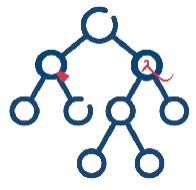
\includegraphics[height=1.0cm]{msca_logo.png}}%
    \end{center}

    \vspace{0.6cm}

    % Main title with Q logos on sides (with clickable links)
    \begin{center}
        \begin{minipage}{0.1\textwidth}
            \centering
            \href{https://quantlet.com}{
\includegraphics[height=1.1cm]{ql_logo.png}}
        \end{minipage}%
        \begin{minipage}{0.78\textwidth}
            \centering
            {\LARGE\bfseries\usebeamercolor[fg]{title}\inserttitle}

            \vspace{0.3cm}

            {\usebeamerfont{subtitle}\usebeamercolor[fg]{title}\insertsubtitle}
        \end{minipage}%
        \begin{minipage}{0.1\textwidth}
            \centering
            \href{https://quantinar.com}{
\includegraphics[height=1.1cm]{qr_logo.png}}
        \end{minipage}
    \end{center}

    \vspace{0.6cm}

    % Authors (left aligned)
    \hspace{0.5cm}{\usebeamerfont{author}\insertauthor}

    \vspace{0.3cm}

    % Institute/Affiliations (left aligned)
    \hspace{0.5cm}\begin{minipage}[t]{0.9\textwidth}
        \raggedright\small\insertinstitute
    \end{minipage}
}

%=============================================================================
% THEOREM ENVIRONMENTS
%=============================================================================
\theoremstyle{definition}
\setbeamertemplate{theorems}[numbered]
\ifdefined\atslang
\newtheorem{defn}{Definiție}
\newtheorem{thm}{Teoremă}
\newtheorem{prop}{Propoziție}
\newtheorem{rmk}{Observație}
\else
\newtheorem{defn}{Definition}
\newtheorem{thm}{Theorem}
\newtheorem{prop}{Proposition}
\newtheorem{rmk}{Remark}
\fi

%=============================================================================
% CENTRED MINIPAGE (no extra vertical space)
%=============================================================================
\newenvironment{cminipage}[1]{%
    \par\noindent\hfill\begin{minipage}{#1}\ignorespaces
}{%
    \end{minipage}\hfill\null\par
}

%=============================================================================
% CUSTOM COMMANDS
%=============================================================================
\newcommand{\E}{\mathbb{E}}
\newcommand{\Var}{\text{Var}}
\newcommand{\Cov}{\text{Cov}}
\newcommand{\Corr}{\text{Corr}}
\newcommand{\R}{\mathbb{R}}
\newcommand{\N}{\mathbb{N}}
\newcommand{\Z}{\mathbb{Z}}
\newcommand{\B}{\mathbf{B}}
\newcommand{\imark}{\textcolor{MainBlue}{\textbullet}}
\newcommand{\RMSE}{\text{RMSE}}
\newcommand{\MAE}{\text{MAE}}
\newcommand{\MAPE}{\text{MAPE}}

% Boldface vector/matrix commands (VAR, VECM, state space)
\newcommand{\bY}{\mathbf{Y}}
\newcommand{\bX}{\mathbf{X}}
\newcommand{\bA}{\mathbf{A}}
\newcommand{\bB}{\mathbf{B}}
\newcommand{\bepsilon}{\boldsymbol{\varepsilon}}
\newcommand{\bSigma}{\boldsymbol{\Sigma}}
\newcommand{\bPhi}{\boldsymbol{\Phi}}
\newcommand{\bGamma}{\boldsymbol{\Gamma}}
\newcommand{\bPi}{\boldsymbol{\Pi}}
\newcommand{\bc}{\mathbf{c}}
\newcommand{\balpha}{\boldsymbol{\alpha}}
\newcommand{\bbeta}{\boldsymbol{\beta}}
\newcommand{\bvarepsilon}{\boldsymbol{\varepsilon}}

% Seminar marks
\newcommand{\correct}{\textcolor{Forest}{\checkmark}}
\newcommand{\incorrect}{\textcolor{Crimson}{\texttimes}}
 se definește
%   \newcommand{\coursename}{Advanced Time Series Analysis and Forecasting}          (EN)
%   \newcommand{\coursename}{Analiza avansată a seriilor de timp și previziune}       (RO)  și  \def\atslang{ro}
% Fișierele .tex se află în EN/Courses, EN/Seminars, RO/Cursuri, RO/Seminarii (două niveluri sub rădăcină).
% Deck-urile sînt generate de latex/build_chapterN.py / build_seminarN.py (vezi latex/ats_build.py).

\documentclass[9pt, aspectratio=169, t]{beamer}
\providecommand{\coursename}{Advanced Time Series Analysis and Forecasting}

% Ensure content fits on slides
\setbeamersize{text margin left=8mm, text margin right=8mm}
% Smaller institute font (title page)
\setbeamerfont{institute}{size=\footnotesize}

%=============================================================================
% THEME AND STYLE CONFIGURATION
%=============================================================================
\usetheme{default}
% Using default theme for clean header/footer control

% Color Palette (matching Redispatch PDF)
\definecolor{MainBlue}{RGB}{26, 58, 110}
\definecolor{AccentBlue}{RGB}{26, 58, 110}
\definecolor{IDAred}{RGB}{205, 0, 0}
\definecolor{DarkGray}{RGB}{51, 51, 51}
\definecolor{MediumGray}{RGB}{128, 128, 128}
\definecolor{LightGray}{RGB}{248, 248, 248}
\definecolor{VeryLightGray}{RGB}{235, 235, 235}
\definecolor{KeynoteGray}{RGB}{218, 218, 218}
\definecolor{SectionGray}{RGB}{120, 120, 120}
\definecolor{FooterGray}{RGB}{100, 100, 100}
\definecolor{Crimson}{RGB}{220, 53, 69}
\definecolor{Forest}{RGB}{46, 125, 50}
\definecolor{Amber}{RGB}{181, 133, 63}
\definecolor{Orange}{RGB}{230, 126, 34}
\definecolor{Purple}{RGB}{142, 68, 173}

% Gradient background (exact Keynote 315° gradient: white to RGB 218,218,218)
\setbeamertemplate{background}{%
    \begin{tikzpicture}[remember picture, overlay]
        \shade[shading=axis, shading angle=315,
        top color=white, bottom color=KeynoteGray]
        (current page.south west) rectangle (current page.north east);
    \end{tikzpicture}%
}
% Fallback solid color for compatibility
\setbeamercolor{background canvas}{bg=}

\setbeamercolor{palette primary}{bg=MainBlue, fg=white}
\setbeamercolor{palette secondary}{bg=MainBlue!85, fg=white}
\setbeamercolor{palette tertiary}{bg=MainBlue!70, fg=white}
\setbeamercolor{structure}{fg=MainBlue}
\setbeamercolor{title}{fg=IDAred}
\setbeamercolor{frametitle}{fg=IDAred, bg=}
\setbeamercolor{block title}{bg=MainBlue, fg=white}
\setbeamercolor{block body}{bg=VeryLightGray, fg=DarkGray}
\setbeamercolor{block title alerted}{bg=Crimson, fg=white}
\setbeamercolor{block body alerted}{bg=Crimson!8, fg=DarkGray}
\setbeamercolor{block title example}{bg=Forest, fg=white}
\setbeamercolor{block body example}{bg=Forest!8, fg=DarkGray}
\setbeamercolor{item}{fg=MainBlue}

% Footer colors (override Madrid theme blue)
\setbeamercolor{author in head/foot}{fg=FooterGray, bg=}
\setbeamercolor{title in head/foot}{fg=FooterGray, bg=}
\setbeamercolor{date in head/foot}{fg=FooterGray, bg=}
\setbeamercolor{section in head/foot}{fg=FooterGray, bg=}
\setbeamercolor{subsection in head/foot}{fg=FooterGray, bg=}

% Bullet styles (apply everywhere including blocks)
\setbeamertemplate{itemize item}{\color{MainBlue}$\boxdot$}
\setbeamertemplate{itemize subitem}{\color{MainBlue}$\blacktriangleright$}
\setbeamertemplate{itemize subsubitem}{\color{MainBlue}\tiny$\bullet$}
\setbeamertemplate{itemize/enumerate body begin}{\normalsize}
\setbeamertemplate{itemize/enumerate subbody begin}{\normalsize}

% Item spacing - compact style
\setlength{\leftmargini}{10pt}       % Level 1: minimal indent
\setlength{\leftmarginii}{10pt}      % Level 2: minimal additional indent
% Compact list spacing (zero extra space before/after lists in blocks)
\makeatletter
\def\@listi{\leftmargin\leftmargini \topsep 0pt \parsep 0pt \itemsep 0pt}
\def\@listii{\leftmargin\leftmarginii \topsep 0pt \parsep 0pt \itemsep 0pt}
\makeatother

\setbeamertemplate{navigation symbols}{}

%=============================================================================
% CUSTOM HEADLINE
%=============================================================================
\setbeamertemplate{headline}{%
    \vskip10pt%
    \hbox to \paperwidth{%
        \hskip0.5cm%
        {\small\color{FooterGray}\renewcommand{\hyperlink}[2]{##2}\insertsectionhead}%
        \hfill%
        \textcolor{FooterGray}{\small\insertframenumber}%
        \hskip0.5cm%
    }%
    \vskip4pt%
    {\color{FooterGray}\hrule height 0.4pt}%
}

%=============================================================================
% CUSTOM FOOTER
%=============================================================================
\usepackage{fontawesome5}

\setbeamertemplate{footline}{%
    {\color{FooterGray}\hrule height 0.4pt}%
    \vskip4pt%
    \hbox to \paperwidth{%
        \hskip0.5cm%
        \textcolor{FooterGray}{\small\coursename}%
        \hfill%
        \raisebox{-0.1em}{%
            \begin{tikzpicture}[x=0.08em, y=0.08em, line width=0.4pt]
                \draw[FooterGray] (0,3) -- (1,4) -- (2,3.5) -- (3,5) -- (4,4) -- (5,6) -- (6,5.5) -- (7,4) -- (8,5) -- (9,7) -- (10,6) -- (11,5) -- (12,6.5) -- (13,8) -- (14,7) -- (15,6) -- (16,7.5) -- (17,9) -- (18,8) -- (19,7) -- (20,8.5) -- (21,10) -- (22,9) -- (23,8) -- (24,9.5);
            \end{tikzpicture}%
        }%
        \hskip0.5cm%
    }%
    \vskip6pt%
}

%=============================================================================
% PACKAGES
%=============================================================================
\usepackage[utf8]{inputenc}
\DeclareUnicodeCharacter{03B1}{\ensuremath{\alpha}}
\usepackage[T1]{fontenc}
\usepackage{amsmath, amssymb, amsthm}
\usepackage{mathtools}
\usepackage{bm}
\usepackage{tikz}
\usetikzlibrary{arrows.meta, positioning, shapes, calc, decorations.pathreplacing, shadings}
\usepackage{booktabs}
\usepackage{multirow}
\usepackage{array}
\usepackage{graphicx}
\usepackage{animate}
\usepackage{hyperref}
\usepackage{colortbl}
\usepackage{listings}
\lstset{language=Python, basicstyle=\ttfamily\scriptsize, keywordstyle=\color{MainBlue}\bfseries,
  commentstyle=\color{Forest}, stringstyle=\color{Crimson}, breaklines=true,
  frame=none, backgroundcolor=\color{VeryLightGray}, xleftmargin=2mm}
\hypersetup{colorlinks=true, linkcolor=MainBlue, urlcolor=MainBlue}
\graphicspath{{../../logos/}{../../charts/}{../../photos/}}
\usepackage{xcolor}
\hfuzz=2pt  % Suppress tiny overfull warnings (<2pt)
\vfuzz=2pt  % Suppress tiny vertical overfull warnings (<2pt)

%=============================================================================
% QUANTLET COMMANDS
%   \quantlet{<displayed name>}{<url>}       (generic)
%   \atsquantlet{Ch_05}{ATS_ch5_garch}       -> https://github.com/danpele/Advanced-Time-Series/tree/main/Quantlets/Ch_05/ATS_ch5_garch
%   \qlurl{<folder>} is defined per chapter by the generator (Quantlets/Ch_NN/<folder>)
%=============================================================================
\newcommand{\atsrepo}{https://github.com/danpele/Advanced-Time-Series}
\newcommand{\atsqlbase}{https://github.com/danpele/Advanced-Time-Series/tree/main/Quantlets}
\newcommand{\quantlet}[2]{%
    \hfill\href{#2}{%
        \raisebox{-0.15em}{
\includegraphics[height=0.7em]{ql_logo.png}}%
        \textcolor{MainBlue}{\tiny\ #1}%
    }%
}
\newcommand{\atsquantlet}[2]{\quantlet{\detokenize{#2}}{\atsqlbase/#1/#2}}

%=============================================================================
% NOTEBOOKS (Google Colab)
%   \colaburl{notebooks/EN/chapter5_seminar_notebook.ipynb} -> the Colab link of a file in the ATS repo
%   \nb: the chapter notebook (each seminar deck redefines it with \renewcommand)
%=============================================================================
\newcommand{\colaburl}[1]{https://colab.research.google.com/github/danpele/Advanced-Time-Series/blob/main/#1}
\newcommand{\nb}{https://colab.research.google.com/github/danpele/Advanced-Time-Series/tree/main/notebooks/EN}
\newcommand{\nbname}{notebooks/EN}

%=============================================================================
% SLIDE HELPERS (used by the generators; the same as in MFM)
%=============================================================================
% local font size for list bodies (the preamble forces \normalsize)
\newcommand{\itemsize}[1]{\setbeamertemplate{itemize/enumerate body begin}{#1}\setbeamertemplate{itemize/enumerate subbody begin}{#1}}
\newcommand{\intitle}[1]{{\hypersetup{urlcolor=white}#1}}   % white links inside coloured title bars
\newcommand{\imgcap}[1]{{\scriptsize #1}\\[0.5mm]}          % caption under a photo
\newcommand{\imgcredit}[2]{{\tiny\color{FooterGray}\href{#1}{#2}}}   % image credit: source URL, author/licence
\newcommand{\aiprompt}[1]{{\ttfamily\color{MainBlue}#1}}     % a prompt to an AI assistant

%=============================================================================
% SEMINARS: student version by default; the instructor wrapper *_solutions.tex sets \solutionstrue
%=============================================================================
\makeatletter\@ifundefined{ifsolutions}{\expandafter\newif\csname ifsolutions\endcsname}{}\makeatother
\newcommand{\solonly}[1]{\ifsolutions #1\fi}
\newcommand{\propsub}{\ifsolutions\else\framesubtitle{\ifdefined\atslang Rezolvarea se discută la seminar\else Solution discussed in class\fi}\fi}

%=============================================================================
% APPENDIX AND CHAPTER LINKS (latex/appendix_links.py writes the calls; it also re-declares these
% macros before \begin{document}, so the decks compile with or without this preamble block)
%=============================================================================
\providecommand{\atsapplink}[3]{\hypertarget{#2}{}\hyperlink{#1}{\beamergotobutton{#3}}}
\providecommand{\atsappback}[2]{\begin{tikzpicture}[remember picture,overlay]\node[anchor=south east] at ([xshift=-3mm,yshift=7mm]current page.south east){\hyperlink{#1}{\beamerreturnbutton{#2}}};\end{tikzpicture}}
\providecommand{\atschlink}[2]{\href{#1}{#2}}
\providecommand{\atschlinkt}[2]{\href{#1}{\usebeamercolor[fg]{frametitle}#2}}

%=============================================================================
% QUANTINAR COMMAND: link către un curs Quantinar (subiecte avansate)
%=============================================================================
\newcommand{\quantinar}[2]{%
    \href{#2}{%
        \raisebox{-0.15em}{
\includegraphics[height=0.8em]{qr_logo.png}}%
        \textcolor{MainBlue}{\scriptsize\ #1}%
    }%
}

%=============================================================================
% CUSTOM TITLE PAGE
%=============================================================================
\defbeamertemplate*{title page}{hybrid}[1][]
{
    \vspace{0.2cm}
    % Logos row - top header (with clickable links)
    \begin{center}
        \href{https://www.ase.ro}{
\includegraphics[height=1.0cm]{ase_logo.png}}\hspace{0.3cm}%
        \href{https://theida.net}{
\includegraphics[height=1.0cm]{ida_logo.png}}\hspace{0.3cm}%
        \href{https://blockchain-research-center.com}{
\includegraphics[height=1.0cm]{brc_logo.png}}\hspace{0.3cm}%
        \href{https://www.ai4efin.ase.ro}{
\includegraphics[height=1.0cm]{ai4efin_logo.png}}\hspace{0.3cm}%
        \href{https://ipe.ro/new}{
\includegraphics[height=1.0cm]{acad_logo.png}}\hspace{0.3cm}%
        \href{https://www.digital-finance-msca.com}{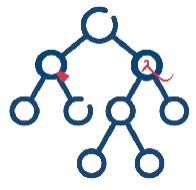
\includegraphics[height=1.0cm]{msca_logo.png}}%
    \end{center}

    \vspace{0.6cm}

    % Main title with Q logos on sides (with clickable links)
    \begin{center}
        \begin{minipage}{0.1\textwidth}
            \centering
            \href{https://quantlet.com}{
\includegraphics[height=1.1cm]{ql_logo.png}}
        \end{minipage}%
        \begin{minipage}{0.78\textwidth}
            \centering
            {\LARGE\bfseries\usebeamercolor[fg]{title}\inserttitle}

            \vspace{0.3cm}

            {\usebeamerfont{subtitle}\usebeamercolor[fg]{title}\insertsubtitle}
        \end{minipage}%
        \begin{minipage}{0.1\textwidth}
            \centering
            \href{https://quantinar.com}{
\includegraphics[height=1.1cm]{qr_logo.png}}
        \end{minipage}
    \end{center}

    \vspace{0.6cm}

    % Authors (left aligned)
    \hspace{0.5cm}{\usebeamerfont{author}\insertauthor}

    \vspace{0.3cm}

    % Institute/Affiliations (left aligned)
    \hspace{0.5cm}\begin{minipage}[t]{0.9\textwidth}
        \raggedright\small\insertinstitute
    \end{minipage}
}

%=============================================================================
% THEOREM ENVIRONMENTS
%=============================================================================
\theoremstyle{definition}
\setbeamertemplate{theorems}[numbered]
\ifdefined\atslang
\newtheorem{defn}{Definiție}
\newtheorem{thm}{Teoremă}
\newtheorem{prop}{Propoziție}
\newtheorem{rmk}{Observație}
\else
\newtheorem{defn}{Definition}
\newtheorem{thm}{Theorem}
\newtheorem{prop}{Proposition}
\newtheorem{rmk}{Remark}
\fi

%=============================================================================
% CENTRED MINIPAGE (no extra vertical space)
%=============================================================================
\newenvironment{cminipage}[1]{%
    \par\noindent\hfill\begin{minipage}{#1}\ignorespaces
}{%
    \end{minipage}\hfill\null\par
}

%=============================================================================
% CUSTOM COMMANDS
%=============================================================================
\newcommand{\E}{\mathbb{E}}
\newcommand{\Var}{\text{Var}}
\newcommand{\Cov}{\text{Cov}}
\newcommand{\Corr}{\text{Corr}}
\newcommand{\R}{\mathbb{R}}
\newcommand{\N}{\mathbb{N}}
\newcommand{\Z}{\mathbb{Z}}
\newcommand{\B}{\mathbf{B}}
\newcommand{\imark}{\textcolor{MainBlue}{\textbullet}}
\newcommand{\RMSE}{\text{RMSE}}
\newcommand{\MAE}{\text{MAE}}
\newcommand{\MAPE}{\text{MAPE}}

% Boldface vector/matrix commands (VAR, VECM, state space)
\newcommand{\bY}{\mathbf{Y}}
\newcommand{\bX}{\mathbf{X}}
\newcommand{\bA}{\mathbf{A}}
\newcommand{\bB}{\mathbf{B}}
\newcommand{\bepsilon}{\boldsymbol{\varepsilon}}
\newcommand{\bSigma}{\boldsymbol{\Sigma}}
\newcommand{\bPhi}{\boldsymbol{\Phi}}
\newcommand{\bGamma}{\boldsymbol{\Gamma}}
\newcommand{\bPi}{\boldsymbol{\Pi}}
\newcommand{\bc}{\mathbf{c}}
\newcommand{\balpha}{\boldsymbol{\alpha}}
\newcommand{\bbeta}{\boldsymbol{\beta}}
\newcommand{\bvarepsilon}{\boldsymbol{\varepsilon}}

% Seminar marks
\newcommand{\correct}{\textcolor{Forest}{\checkmark}}
\newcommand{\incorrect}{\textcolor{Crimson}{\texttimes}}
 se definește
%   \newcommand{\coursename}{Advanced Time Series Analysis and Forecasting}          (EN)
%   \newcommand{\coursename}{Analiza avansată a seriilor de timp și previziune}       (RO)  și  \def\atslang{ro}
% Fișierele .tex se află în EN/Courses, EN/Seminars, RO/Cursuri, RO/Seminarii (două niveluri sub rădăcină).
% Deck-urile sînt generate de latex/build_chapterN.py / build_seminarN.py (vezi latex/ats_build.py).

\documentclass[9pt, aspectratio=169, t]{beamer}
\providecommand{\coursename}{Advanced Time Series Analysis and Forecasting}

% Ensure content fits on slides
\setbeamersize{text margin left=8mm, text margin right=8mm}
% Smaller institute font (title page)
\setbeamerfont{institute}{size=\footnotesize}

%=============================================================================
% THEME AND STYLE CONFIGURATION
%=============================================================================
\usetheme{default}
% Using default theme for clean header/footer control

% Color Palette (matching Redispatch PDF)
\definecolor{MainBlue}{RGB}{26, 58, 110}
\definecolor{AccentBlue}{RGB}{26, 58, 110}
\definecolor{IDAred}{RGB}{205, 0, 0}
\definecolor{DarkGray}{RGB}{51, 51, 51}
\definecolor{MediumGray}{RGB}{128, 128, 128}
\definecolor{LightGray}{RGB}{248, 248, 248}
\definecolor{VeryLightGray}{RGB}{235, 235, 235}
\definecolor{KeynoteGray}{RGB}{218, 218, 218}
\definecolor{SectionGray}{RGB}{120, 120, 120}
\definecolor{FooterGray}{RGB}{100, 100, 100}
\definecolor{Crimson}{RGB}{220, 53, 69}
\definecolor{Forest}{RGB}{46, 125, 50}
\definecolor{Amber}{RGB}{181, 133, 63}
\definecolor{Orange}{RGB}{230, 126, 34}
\definecolor{Purple}{RGB}{142, 68, 173}

% Gradient background (exact Keynote 315° gradient: white to RGB 218,218,218)
\setbeamertemplate{background}{%
    \begin{tikzpicture}[remember picture, overlay]
        \shade[shading=axis, shading angle=315,
        top color=white, bottom color=KeynoteGray]
        (current page.south west) rectangle (current page.north east);
    \end{tikzpicture}%
}
% Fallback solid color for compatibility
\setbeamercolor{background canvas}{bg=}

\setbeamercolor{palette primary}{bg=MainBlue, fg=white}
\setbeamercolor{palette secondary}{bg=MainBlue!85, fg=white}
\setbeamercolor{palette tertiary}{bg=MainBlue!70, fg=white}
\setbeamercolor{structure}{fg=MainBlue}
\setbeamercolor{title}{fg=IDAred}
\setbeamercolor{frametitle}{fg=IDAred, bg=}
\setbeamercolor{block title}{bg=MainBlue, fg=white}
\setbeamercolor{block body}{bg=VeryLightGray, fg=DarkGray}
\setbeamercolor{block title alerted}{bg=Crimson, fg=white}
\setbeamercolor{block body alerted}{bg=Crimson!8, fg=DarkGray}
\setbeamercolor{block title example}{bg=Forest, fg=white}
\setbeamercolor{block body example}{bg=Forest!8, fg=DarkGray}
\setbeamercolor{item}{fg=MainBlue}

% Footer colors (override Madrid theme blue)
\setbeamercolor{author in head/foot}{fg=FooterGray, bg=}
\setbeamercolor{title in head/foot}{fg=FooterGray, bg=}
\setbeamercolor{date in head/foot}{fg=FooterGray, bg=}
\setbeamercolor{section in head/foot}{fg=FooterGray, bg=}
\setbeamercolor{subsection in head/foot}{fg=FooterGray, bg=}

% Bullet styles (apply everywhere including blocks)
\setbeamertemplate{itemize item}{\color{MainBlue}$\boxdot$}
\setbeamertemplate{itemize subitem}{\color{MainBlue}$\blacktriangleright$}
\setbeamertemplate{itemize subsubitem}{\color{MainBlue}\tiny$\bullet$}
\setbeamertemplate{itemize/enumerate body begin}{\normalsize}
\setbeamertemplate{itemize/enumerate subbody begin}{\normalsize}

% Item spacing - compact style
\setlength{\leftmargini}{10pt}       % Level 1: minimal indent
\setlength{\leftmarginii}{10pt}      % Level 2: minimal additional indent
% Compact list spacing (zero extra space before/after lists in blocks)
\makeatletter
\def\@listi{\leftmargin\leftmargini \topsep 0pt \parsep 0pt \itemsep 0pt}
\def\@listii{\leftmargin\leftmarginii \topsep 0pt \parsep 0pt \itemsep 0pt}
\makeatother

\setbeamertemplate{navigation symbols}{}

%=============================================================================
% CUSTOM HEADLINE
%=============================================================================
\setbeamertemplate{headline}{%
    \vskip10pt%
    \hbox to \paperwidth{%
        \hskip0.5cm%
        {\small\color{FooterGray}\renewcommand{\hyperlink}[2]{##2}\insertsectionhead}%
        \hfill%
        \textcolor{FooterGray}{\small\insertframenumber}%
        \hskip0.5cm%
    }%
    \vskip4pt%
    {\color{FooterGray}\hrule height 0.4pt}%
}

%=============================================================================
% CUSTOM FOOTER
%=============================================================================
\usepackage{fontawesome5}

\setbeamertemplate{footline}{%
    {\color{FooterGray}\hrule height 0.4pt}%
    \vskip4pt%
    \hbox to \paperwidth{%
        \hskip0.5cm%
        \textcolor{FooterGray}{\small\coursename}%
        \hfill%
        \raisebox{-0.1em}{%
            \begin{tikzpicture}[x=0.08em, y=0.08em, line width=0.4pt]
                \draw[FooterGray] (0,3) -- (1,4) -- (2,3.5) -- (3,5) -- (4,4) -- (5,6) -- (6,5.5) -- (7,4) -- (8,5) -- (9,7) -- (10,6) -- (11,5) -- (12,6.5) -- (13,8) -- (14,7) -- (15,6) -- (16,7.5) -- (17,9) -- (18,8) -- (19,7) -- (20,8.5) -- (21,10) -- (22,9) -- (23,8) -- (24,9.5);
            \end{tikzpicture}%
        }%
        \hskip0.5cm%
    }%
    \vskip6pt%
}

%=============================================================================
% PACKAGES
%=============================================================================
\usepackage[utf8]{inputenc}
\DeclareUnicodeCharacter{03B1}{\ensuremath{\alpha}}
\usepackage[T1]{fontenc}
\usepackage{amsmath, amssymb, amsthm}
\usepackage{mathtools}
\usepackage{bm}
\usepackage{tikz}
\usetikzlibrary{arrows.meta, positioning, shapes, calc, decorations.pathreplacing, shadings}
\usepackage{booktabs}
\usepackage{multirow}
\usepackage{array}
\usepackage{graphicx}
\usepackage{animate}
\usepackage{hyperref}
\usepackage{colortbl}
\usepackage{listings}
\lstset{language=Python, basicstyle=\ttfamily\scriptsize, keywordstyle=\color{MainBlue}\bfseries,
  commentstyle=\color{Forest}, stringstyle=\color{Crimson}, breaklines=true,
  frame=none, backgroundcolor=\color{VeryLightGray}, xleftmargin=2mm}
\hypersetup{colorlinks=true, linkcolor=MainBlue, urlcolor=MainBlue}
\graphicspath{{../../logos/}{../../charts/}{../../photos/}}
\usepackage{xcolor}
\hfuzz=2pt  % Suppress tiny overfull warnings (<2pt)
\vfuzz=2pt  % Suppress tiny vertical overfull warnings (<2pt)

%=============================================================================
% QUANTLET COMMANDS
%   \quantlet{<displayed name>}{<url>}       (generic)
%   \atsquantlet{Ch_05}{ATS_ch5_garch}       -> https://github.com/danpele/Advanced-Time-Series/tree/main/Quantlets/Ch_05/ATS_ch5_garch
%   \qlurl{<folder>} is defined per chapter by the generator (Quantlets/Ch_NN/<folder>)
%=============================================================================
\newcommand{\atsrepo}{https://github.com/danpele/Advanced-Time-Series}
\newcommand{\atsqlbase}{https://github.com/danpele/Advanced-Time-Series/tree/main/Quantlets}
\newcommand{\quantlet}[2]{%
    \hfill\href{#2}{%
        \raisebox{-0.15em}{
\includegraphics[height=0.7em]{ql_logo.png}}%
        \textcolor{MainBlue}{\tiny\ #1}%
    }%
}
\newcommand{\atsquantlet}[2]{\quantlet{\detokenize{#2}}{\atsqlbase/#1/#2}}

%=============================================================================
% NOTEBOOKS (Google Colab)
%   \colaburl{notebooks/EN/chapter5_seminar_notebook.ipynb} -> the Colab link of a file in the ATS repo
%   \nb: the chapter notebook (each seminar deck redefines it with \renewcommand)
%=============================================================================
\newcommand{\colaburl}[1]{https://colab.research.google.com/github/danpele/Advanced-Time-Series/blob/main/#1}
\newcommand{\nb}{https://colab.research.google.com/github/danpele/Advanced-Time-Series/tree/main/notebooks/EN}
\newcommand{\nbname}{notebooks/EN}

%=============================================================================
% SLIDE HELPERS (used by the generators; the same as in MFM)
%=============================================================================
% local font size for list bodies (the preamble forces \normalsize)
\newcommand{\itemsize}[1]{\setbeamertemplate{itemize/enumerate body begin}{#1}\setbeamertemplate{itemize/enumerate subbody begin}{#1}}
\newcommand{\intitle}[1]{{\hypersetup{urlcolor=white}#1}}   % white links inside coloured title bars
\newcommand{\imgcap}[1]{{\scriptsize #1}\\[0.5mm]}          % caption under a photo
\newcommand{\imgcredit}[2]{{\tiny\color{FooterGray}\href{#1}{#2}}}   % image credit: source URL, author/licence
\newcommand{\aiprompt}[1]{{\ttfamily\color{MainBlue}#1}}     % a prompt to an AI assistant

%=============================================================================
% SEMINARS: student version by default; the instructor wrapper *_solutions.tex sets \solutionstrue
%=============================================================================
\makeatletter\@ifundefined{ifsolutions}{\expandafter\newif\csname ifsolutions\endcsname}{}\makeatother
\newcommand{\solonly}[1]{\ifsolutions #1\fi}
\newcommand{\propsub}{\ifsolutions\else\framesubtitle{\ifdefined\atslang Rezolvarea se discută la seminar\else Solution discussed in class\fi}\fi}

%=============================================================================
% APPENDIX AND CHAPTER LINKS (latex/appendix_links.py writes the calls; it also re-declares these
% macros before \begin{document}, so the decks compile with or without this preamble block)
%=============================================================================
\providecommand{\atsapplink}[3]{\hypertarget{#2}{}\hyperlink{#1}{\beamergotobutton{#3}}}
\providecommand{\atsappback}[2]{\begin{tikzpicture}[remember picture,overlay]\node[anchor=south east] at ([xshift=-3mm,yshift=7mm]current page.south east){\hyperlink{#1}{\beamerreturnbutton{#2}}};\end{tikzpicture}}
\providecommand{\atschlink}[2]{\href{#1}{#2}}
\providecommand{\atschlinkt}[2]{\href{#1}{\usebeamercolor[fg]{frametitle}#2}}

%=============================================================================
% QUANTINAR COMMAND: link către un curs Quantinar (subiecte avansate)
%=============================================================================
\newcommand{\quantinar}[2]{%
    \href{#2}{%
        \raisebox{-0.15em}{
\includegraphics[height=0.8em]{qr_logo.png}}%
        \textcolor{MainBlue}{\scriptsize\ #1}%
    }%
}

%=============================================================================
% CUSTOM TITLE PAGE
%=============================================================================
\defbeamertemplate*{title page}{hybrid}[1][]
{
    \vspace{0.2cm}
    % Logos row - top header (with clickable links)
    \begin{center}
        \href{https://www.ase.ro}{
\includegraphics[height=1.0cm]{ase_logo.png}}\hspace{0.3cm}%
        \href{https://theida.net}{
\includegraphics[height=1.0cm]{ida_logo.png}}\hspace{0.3cm}%
        \href{https://blockchain-research-center.com}{
\includegraphics[height=1.0cm]{brc_logo.png}}\hspace{0.3cm}%
        \href{https://www.ai4efin.ase.ro}{
\includegraphics[height=1.0cm]{ai4efin_logo.png}}\hspace{0.3cm}%
        \href{https://ipe.ro/new}{
\includegraphics[height=1.0cm]{acad_logo.png}}\hspace{0.3cm}%
        \href{https://www.digital-finance-msca.com}{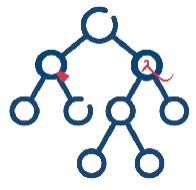
\includegraphics[height=1.0cm]{msca_logo.png}}%
    \end{center}

    \vspace{0.6cm}

    % Main title with Q logos on sides (with clickable links)
    \begin{center}
        \begin{minipage}{0.1\textwidth}
            \centering
            \href{https://quantlet.com}{
\includegraphics[height=1.1cm]{ql_logo.png}}
        \end{minipage}%
        \begin{minipage}{0.78\textwidth}
            \centering
            {\LARGE\bfseries\usebeamercolor[fg]{title}\inserttitle}

            \vspace{0.3cm}

            {\usebeamerfont{subtitle}\usebeamercolor[fg]{title}\insertsubtitle}
        \end{minipage}%
        \begin{minipage}{0.1\textwidth}
            \centering
            \href{https://quantinar.com}{
\includegraphics[height=1.1cm]{qr_logo.png}}
        \end{minipage}
    \end{center}

    \vspace{0.6cm}

    % Authors (left aligned)
    \hspace{0.5cm}{\usebeamerfont{author}\insertauthor}

    \vspace{0.3cm}

    % Institute/Affiliations (left aligned)
    \hspace{0.5cm}\begin{minipage}[t]{0.9\textwidth}
        \raggedright\small\insertinstitute
    \end{minipage}
}

%=============================================================================
% THEOREM ENVIRONMENTS
%=============================================================================
\theoremstyle{definition}
\setbeamertemplate{theorems}[numbered]
\ifdefined\atslang
\newtheorem{defn}{Definiție}
\newtheorem{thm}{Teoremă}
\newtheorem{prop}{Propoziție}
\newtheorem{rmk}{Observație}
\else
\newtheorem{defn}{Definition}
\newtheorem{thm}{Theorem}
\newtheorem{prop}{Proposition}
\newtheorem{rmk}{Remark}
\fi

%=============================================================================
% CENTRED MINIPAGE (no extra vertical space)
%=============================================================================
\newenvironment{cminipage}[1]{%
    \par\noindent\hfill\begin{minipage}{#1}\ignorespaces
}{%
    \end{minipage}\hfill\null\par
}

%=============================================================================
% CUSTOM COMMANDS
%=============================================================================
\newcommand{\E}{\mathbb{E}}
\newcommand{\Var}{\text{Var}}
\newcommand{\Cov}{\text{Cov}}
\newcommand{\Corr}{\text{Corr}}
\newcommand{\R}{\mathbb{R}}
\newcommand{\N}{\mathbb{N}}
\newcommand{\Z}{\mathbb{Z}}
\newcommand{\B}{\mathbf{B}}
\newcommand{\imark}{\textcolor{MainBlue}{\textbullet}}
\newcommand{\RMSE}{\text{RMSE}}
\newcommand{\MAE}{\text{MAE}}
\newcommand{\MAPE}{\text{MAPE}}

% Boldface vector/matrix commands (VAR, VECM, state space)
\newcommand{\bY}{\mathbf{Y}}
\newcommand{\bX}{\mathbf{X}}
\newcommand{\bA}{\mathbf{A}}
\newcommand{\bB}{\mathbf{B}}
\newcommand{\bepsilon}{\boldsymbol{\varepsilon}}
\newcommand{\bSigma}{\boldsymbol{\Sigma}}
\newcommand{\bPhi}{\boldsymbol{\Phi}}
\newcommand{\bGamma}{\boldsymbol{\Gamma}}
\newcommand{\bPi}{\boldsymbol{\Pi}}
\newcommand{\bc}{\mathbf{c}}
\newcommand{\balpha}{\boldsymbol{\alpha}}
\newcommand{\bbeta}{\boldsymbol{\beta}}
\newcommand{\bvarepsilon}{\boldsymbol{\varepsilon}}

% Seminar marks
\newcommand{\correct}{\textcolor{Forest}{\checkmark}}
\newcommand{\incorrect}{\textcolor{Crimson}{\texttimes}}


\newcommand{\qlurl}[1]{https://github.com/danpele/Advanced-Time-Series/tree/main/Quantlets/Ch_09/#1}

% Clickable citations (DOIs verified via Crossref)
\newcommand{\refAT}{\href{https://doi.org/10.1016/S0378-4266(02)00283-2}{Acerbi and Tasche (2002)}}
\newcommand{\refAS}{\href{https://www.msci.com/documents/10199/22aa9922-f874-4060-b77a-0f0e267a489b}{Acerbi and Székely (2014)}}
\newcommand{\refADEH}{\href{https://doi.org/10.1111/1467-9965.00068}{Artzner et al.\ (1999)}}
\newcommand{\refBCBS}{\href{https://www.bis.org/publ/bcbs22.htm}{Basel Committee (1996)}}
\newcommand{\refMAR}{\href{https://www.bis.org/basel_framework/chapter/MAR/33.htm}{Basel Committee (MAR33)}}
\newcommand{\refBD}{\href{https://doi.org/10.1093/jjfinec/nbaa013}{Bayer and Dimitriadis (2022)}}
\newcommand{\refBoll}{\href{https://doi.org/10.1016/0304-4076(86)90063-1}{Bollerslev (1986)}}
\newcommand{\refBDKM}{\href{https://doi.org/10.1016/j.jbankfin.2014.03.019}{Boucher et al.\ (2014)}}
\newcommand{\refChr}{\href{https://doi.org/10.2307/2527341}{Christoffersen (1998)}}
\newcommand{\refCG}{\href{https://doi.org/10.21314/JOR.2005.112}{Christoffersen and Gonçalves (2005)}}
\newcommand{\refCP}{\href{https://doi.org/10.1093/jjfinec/nbh004}{Christoffersen and Pelletier (2004)}}
\newcommand{\refCKL}{\href{https://doi.org/10.1002/jae.1279}{Creal, Koopman and Lucas (2013)}}
\newcommand{\refDJVZ}{\href{https://doi.org/10.1016/j.jfs.2016.02.002}{Danielsson et al.\ (2016)}}
\newcommand{\refDZ}{\href{https://doi.org/10.1016/j.jbankfin.2005.10.002}{Daníelsson and Zigrand (2006)}}
\newcommand{\refDM}{\href{https://doi.org/10.1080/07350015.1995.10524599}{Diebold and Mariano (1995)}}
\newcommand{\refDB}{\href{https://doi.org/10.1214/19-EJS1560}{Dimitriadis and Bayer (2019)}}
\newcommand{\refDE}{\href{https://doi.org/10.1287/mnsc.2015.2342}{Du and Escanciano (2017)}}
\newcommand{\refEGJK}{\href{https://doi.org/10.1111/rssb.12154}{Ehm et al.\ (2016)}}
\newcommand{\refEKM}{\href{https://doi.org/10.1007/978-3-642-33483-2}{Embrechts, Klüppelberg and Mikosch (1997)}}
\newcommand{\refEM}{\href{https://doi.org/10.1198/073500104000000370}{Engle and Manganelli (2004)}}
\newcommand{\refEO}{\href{https://doi.org/10.1198/jbes.2009.07063}{Escanciano and Olmo (2010)}}
\newcommand{\refFS}{\href{https://doi.org/10.1111/1467-9868.00401}{Ferro and Segers (2003)}}
\newcommand{\refFZ}{\href{https://doi.org/10.1214/16-AOS1439}{Fissler and Ziegel (2016)}}
\newcommand{\refFZG}{\href{https://arxiv.org/abs/1507.00244}{Fissler, Ziegel and Gneiting (2016)}}
\newcommand{\refGLLS}{\href{https://doi.org/10.1198/jbes.2010.07318}{Gaglianone et al.\ (2011)}}
\newcommand{\refGS}{\href{https://doi.org/10.1017/S0266466608080559}{Gao and Song (2008)}}
\newcommand{\refGC}{\href{https://arxiv.org/abs/2106.00170}{Gibbs and Candès (2021)}}
\newcommand{\refGW}{\href{https://doi.org/10.1111/j.1468-0262.2006.00718.x}{Giacomini and White (2006)}}
\newcommand{\refGJR}{\href{https://doi.org/10.1111/j.1540-6261.1993.tb05128.x}{Glosten, Jagannathan and Runkle (1993)}}
\newcommand{\refGn}{\href{https://doi.org/10.1198/jasa.2011.r10138}{Gneiting (2011)}}
\newcommand{\refGR}{\href{https://doi.org/10.1198/016214506000001437}{Gneiting and Raftery (2007)}}
\newcommand{\refHan}{\href{https://doi.org/10.2307/2527081}{Hansen (1994)}}
\newcommand{\refHLN}{\href{https://doi.org/10.3982/ECTA5771}{Hansen, Lunde and Nason (2011)}}
\newcommand{\refHE}{\href{https://doi.org/10.1214/13-AOAS709}{Holzmann and Eulert (2014)}}
\newcommand{\refKR}{\href{https://doi.org/10.1016/j.jedc.2016.05.002}{Kellner and Rösch (2016)}}
\newcommand{\refKB}{\href{https://doi.org/10.2307/1913643}{Koenker and Bassett (1978)}}
\newcommand{\refKoe}{\href{https://doi.org/10.1017/CBO9780511754098}{Koenker (2005)}}
\newcommand{\refKX}{\href{https://doi.org/10.1198/016214506000000672}{Koenker and Xiao (2006)}}
\newcommand{\refKLM}{\href{https://doi.org/10.1016/j.jbankfin.2018.01.002}{Kratz, Lok and McNeil (2018)}}
\newcommand{\refKup}{\href{https://doi.org/10.3905/jod.1995.407942}{Kupiec (1995)}}
\newcommand{\refMF}{\href{https://doi.org/10.1016/S0927-5398(00)00012-8}{McNeil and Frey (2000)}}
\newcommand{\refNZ}{\href{https://doi.org/10.1214/17-AOAS1041}{Nolde and Ziegel (2017)}}
\newcommand{\refPZC}{\href{https://doi.org/10.1016/j.jeconom.2018.10.008}{Patton, Ziegel and Chen (2019)}}
\newcommand{\refPet}{\href{https://doi.org/10.1016/j.ijforecast.2021.11.001}{Petropoulos et al.\ (2022)}}
\newcommand{\refTayA}{\href{https://doi.org/10.1093/jjfinec/nbn001}{Taylor (2008)}}
\newcommand{\refTayB}{\href{https://doi.org/10.1080/07350015.2017.1281815}{Taylor (2019)}}
\newcommand{\refWeb}{\href{https://doi.org/10.1111/j.1467-9965.2006.00277.x}{Weber (2006)}}
\newcommand{\refZie}{\href{https://doi.org/10.1111/mafi.12080}{Ziegel (2016)}}
\newcommand{\refCO}{\href{https://github.com/danpele/Conformal_Oracle}{Pele et al.\ (Conformal\_Oracle)}}

\title[Advanced Time Series Analysis and Forecasting]{Advanced Time Series Analysis and Forecasting}
\subtitle{Chapter 9: VaR, ES and backtesting: elicitability, scoring and model risk}
\author[D.T. Pele]{Daniel Traian PELE}
\institute{Bucharest University of Economic Studies\\
IDA Institute Digital Assets\\
Blockchain Research Center\\
AI4EFin Artificial Intelligence for Energy Finance\\
Romanian Academy, Institute for Economic Forecasting\\
MSCA Digital Finance}
\date{}

%=============================================================================
\providecommand{\atsapplink}[3]{\hypertarget{#2}{}\hyperlink{#1}{\beamergotobutton{#3}}}  % APPLINKS-MACROS
\providecommand{\atsappback}[2]{\begin{tikzpicture}[remember picture,overlay]\node[anchor=south east] at ([xshift=-3mm,yshift=7mm]current page.south east){\hyperlink{#1}{\beamerreturnbutton{#2}}};\end{tikzpicture}}  % APPLINKS-MACROS
\providecommand{\atschlink}[2]{\href{#1}{#2}}  % APPLINKS-MACROS
\providecommand{\atschlinkt}[2]{\href{#1}{\usebeamercolor[fg]{frametitle}#2}}  % APPLINKS-MACROS
\begin{document}
%=============================================================================

{
\setbeamertemplate{headline}{}
\setbeamertemplate{footline}{}
\begin{frame}[noframenumbering]
    \titlepage
\end{frame}
}
% BEGIN-ACRONYMS (generat de latex/acronyms.py; nu editati manual)
\begin{frame}{Acronyms used in this material (1/3)}
\setbeamertemplate{itemize/enumerate body begin}{\footnotesize}
\begin{columns}[T]
\begin{column}{0.49\textwidth}
\begin{itemize}\setlength{\itemsep}{0pt}
    \item \textbf{ACI}: Adaptive Conformal Inference
    \item \textbf{ADAPT}: Adaptive (CAViaR specification)
    \item \textbf{AI}: Artificial Intelligence
    \item \textbf{AR}: AutoRegressive (model); in event studies: Abnormal Return
    \item \textbf{ARFIMA}: AutoRegressive Fractionally Integrated Moving Average (model)
    \item \textbf{ARMA}: AutoRegressive Moving Average (model)
    \item \textbf{ARMA-GARCH}: ARMA mean with GARCH variance
    \item \textbf{AS}: Asymmetric Slope (CAViaR specification)
    \item \textbf{BET}: Bucharest Exchange Trading (index)
    \item \textbf{BIC}: Bayesian Information Criterion
    \item \textbf{BNR}: Banca Națională a României (the National Bank of Romania)
    \item \textbf{BUX}: Budapesti Értéktőzsde index (the Budapest Stock Exchange index)
\end{itemize}
\end{column}
\begin{column}{0.49\textwidth}
\begin{itemize}\setlength{\itemsep}{0pt}
    \item \textbf{DM}: Diebold–Mariano (test)
    \item \textbf{DQ}: Dynamic Quantile (test of Engle and Manganelli)
    \item \textbf{EDF}: Empirical Distribution Function
    \item \textbf{EM}: Engle and Manganelli (2004), CAViaR
    \item \textbf{EODHD}: EOD Historical Data (market-data provider)
    \item \textbf{ES}: Expected Shortfall
    \item \textbf{EVT}: Extreme Value Theory
    \item \textbf{EWMA}: Exponentially Weighted Moving Average
    \item \textbf{FHS}: Filtered Historical Simulation
    \item \textbf{FZ}: Fissler–Ziegel (class of scoring functions for VaR and ES)
    \item \textbf{FZ-1F}: One-factor GAS model for VaR and ES (label of Patton, Ziegel and Chen)
    \item \textbf{FZ-2F}: Two-factor GAS model for VaR and ES (label of Patton, Ziegel and Chen)
\end{itemize}
\end{column}
\end{columns}
\end{frame}
\begin{frame}{Acronyms used in this material (2/3)}
\setbeamertemplate{itemize/enumerate body begin}{\footnotesize}
\begin{columns}[T]
\begin{column}{0.49\textwidth}
\begin{itemize}\setlength{\itemsep}{0pt}
    \item \textbf{FZ0}: Zero-homogeneous Fissler–Ziegel loss (Patton, Ziegel and Chen)
    \item \textbf{GARCH}: Generalised AutoRegressive Conditional Heteroskedasticity
    \item \textbf{GARCH-EDF}: GARCH with innovations from the empirical distribution function
    \item \textbf{GARCH-FZ}: GARCH model estimated by FZ0 minimisation
    \item \textbf{GARCH-N}: GARCH with Normal innovations
    \item \textbf{GAS}: Generalised Autoregressive Score (model)
    \item \textbf{GAS-1F}: One-factor GAS model for VaR and ES
    \item \textbf{GAS-2F}: Two-factor GAS model for VaR and ES
    \item \textbf{GAS-FZ}: GAS models for VaR and ES driven by the FZ0 loss
    \item \textbf{GCH}: GARCH (short label in tables)
    \item \textbf{GCH-EDF}: ARMA-GARCH with innovations from the empirical distribution function
\end{itemize}
\end{column}
\begin{column}{0.49\textwidth}
\begin{itemize}\setlength{\itemsep}{0pt}
    \item \textbf{GCH-FZ}: GARCH model estimated by FZ0 minimisation (table label)
    \item \textbf{GCH-N}: ARMA-GARCH with Normal innovations
    \item \textbf{GJR}: Glosten–Jagannathan–Runkle (asymmetric GARCH)
    \item \textbf{GJR-GARCH}: Glosten–Jagannathan–Runkle GARCH
    \item \textbf{GM}: General Motors (stock)
    \item \textbf{GPL}: Generalised Piecewise Linear (scoring function)
    \item \textbf{GW}: Giacomini–White (test of conditional predictive ability)
    \item \textbf{HAC}: Heteroskedasticity and Autocorrelation Consistent (standard errors)
    \item \textbf{HC0}: Heteroskedasticity-Consistent covariance of White (type 0)
    \item \textbf{HS}: Historical Simulation
    \item \textbf{IBM}: International Business Machines (stock)
\end{itemize}
\end{column}
\end{columns}
\end{frame}
\begin{frame}{Acronyms used in this material (3/3)}
\setbeamertemplate{itemize/enumerate body begin}{\footnotesize}
\begin{columns}[T]
\begin{column}{0.49\textwidth}
\begin{itemize}\setlength{\itemsep}{0pt}
    \item \textbf{IG}: Indirect GARCH (CAViaR specification)
    \item \textbf{LLM}: Large Language Model
    \item \textbf{LR}: Likelihood Ratio (test)
    \item \textbf{MA}: Moving Average
    \item \textbf{MAR33}: Basel Framework, chapter MAR33 (internal models, capital requirements)
    \item \textbf{MCS}: Model Confidence Set
    \item \textbf{MFM}: Modelling Financial Markets
    \item \textbf{MLE}: Maximum Likelihood Estimation
    \item \textbf{MSE}: Mean Squared Error
    \item \textbf{PIT}: Probability Integral Transform
    \item \textbf{PX}: Prague Stock Exchange index (index Burzy cenných papírů Praha)
    \item \textbf{PZC}: Patton, Ziegel and Chen (2019)
    \item \textbf{QLIKE}: Quasi-LIKElihood loss
    \item \textbf{QML}: Quasi-Maximum Likelihood
\end{itemize}
\end{column}
\begin{column}{0.49\textwidth}
\begin{itemize}\setlength{\itemsep}{0pt}
    \item \textbf{RQ}: Regression Quantile (criterion of Engle and Manganelli)
    \item \textbf{RW}: Random Walk
    \item \textbf{RW-125}: Rolling Window of 125 days (historical simulation)
    \item \textbf{RW-250}: Rolling Window of 250 days (historical simulation)
    \item \textbf{RW-500}: Rolling Window of 500 days (historical simulation)
    \item \textbf{SAV}: Symmetric Absolute Value (CAViaR specification)
    \item \textbf{TSA}: Time Series Analysis
    \item \textbf{VAR}: Vector AutoRegression
    \item \textbf{VIX}: CBOE Volatility IndeX
    \item \textbf{WIG20}: Warszawski Indeks Giełdowy 20 (the Warsaw Stock Exchange index of the 20 largest companies)
\end{itemize}
\end{column}
\end{columns}
\end{frame}
% END-ACRONYMS

\begin{frame}{Today's question and route}
\itemsize{\small}
\begin{itemize}
    \item \textbf{Question}: a VaR or an ES forecast is a point forecast of a tail functional; how do we estimate dynamic models for it, test whether it is calibrated and decide which forecast is better?
    \begin{itemize}
        \item the tail is observed rarely: a forecast must be judged with a loss that is consistent for its target, on few informative days
    \end{itemize}
    \item \textbf{Route} of the chapter
    \begin{itemize}
        \item risk measures as functionals; elicitability, the Fissler--Ziegel class, FZ0 and Murphy diagrams
        \item quantile regression and CAViaR; semiparametric (VaR, ES) models and joint regression
        \item backtesting as conditional calibration; estimation risk in backtests; comparison with the MCS in stress periods
        \item the horizon (square-root-of-time), model risk, extremes under dependence, conformal calibration
    \end{itemize}
    \item We build on \atschlink{https://danpele.github.io/Advanced-Time-Series/EN/Courses/chapter1_forecast_evaluation.pdf}{Chapter 1} (scoring rules, elicitability, DM, MCS), \atschlink{https://danpele.github.io/Advanced-Time-Series/EN/Courses/chapter0_refresher_inference.pdf}{Chapter 0} (HAC, bootstrap), \atschlink{https://danpele.github.io/Advanced-Time-Series/EN/Courses/chapter8_advanced_volatility.pdf}{Chapter 8} (volatility) and \atschlink{https://danpele.github.io/Time-Series-Analysis/EN/Courses/chapter5_conditional_volatility_garch.pdf}{TSA, Chapter 5} (GARCH); Seminar 9 comes before this lecture
\end{itemize}
\end{frame}

\begin{frame}{Learning outcomes}
\itemsize{\small}
\begin{itemize}
    \item Characterise the scoring functions consistent for quantiles and for the pair (VaR, ES), and prove that ES alone is not elicitable
    \item Estimate CAViaR models with the Engle--Manganelli procedure, compute their standard errors and run the DQ test
    \item Estimate semiparametric dynamic (VaR, ES) models by FZ0 minimisation and replicate the out-of-sample comparison of Patton, Ziegel and Chen
    \item Test conditional calibration with identification functions, account for estimation risk, and compare risk models with DM tests, Murphy diagrams and the MCS
    \item Quantify horizon, model and estimation risk, and correct a miscalibrated VaR by adaptive conformal inference
\end{itemize}
\end{frame}

\begin{frame}{Reading, data and tools}
\itemsize{\small}
\begin{itemize}
    \item Theory: \refGn; \refFZ; \refEGJK; \refNZ
    \begin{itemize}
        \item Models: \refKB; \refEM; \refPZC; \refDB
        \item Survey of forecasting practice: \refPet
    \end{itemize}
    \item Python Quantlets of this chapter: \href{https://github.com/danpele/Advanced-Time-Series/tree/main/Quantlets/Ch_09}{Quantlets/Ch\_09}
    \begin{itemize}
        \item CAViaR, the GAS-FZ models, the joint regression, the backtests, DM and the MCS written in \texttt{numpy}/\texttt{scipy}; \texttt{numba} only speeds up the recursions
    \end{itemize}
    \item Lecture notebook: \href{\colaburl{notebooks/EN/chapter9_lecture_notebook.ipynb}}{open in Google Colab}
\end{itemize}
\end{frame}

\begin{frame}{Data used in this chapter}
\itemsize{\footnotesize}
\begin{center}
\scriptsize
\begin{tabular}{>{\raggedright\arraybackslash}p{3.0cm}>{\raggedright\arraybackslash}p{4.6cm}>{\raggedright\arraybackslash}p{4.4cm}}
\toprule
\textbf{Series} & \textbf{Source, sample} & \textbf{In sample / out of sample} \\
\midrule
S\&P 500, DAX & EODHD daily closes, January 1990 -- September 2026 & 1990--1999 / 2000--2026 \\
BET & EODHD, official closes, 2000--2026 & 2000--2009 / 2010--2026 \\
EUR/RON & BNR reference rate, July 2005 -- September 2026 & to June 2015 / from July 2015 \\
Bitcoin & EODHD, 7 days a week, September 2014 -- September 2026 & 2014--2019 / 2020--2026 \\
VIX & EODHD daily closes & regressor of the joint (VaR, ES) regression \\
\bottomrule
\end{tabular}
\end{center}
\begin{itemize}
    \item Daily log returns in \%; ten in-sample years as in Patton, Ziegel and Chen (2019), five for Bitcoin; stress periods: September 2008 -- March 2009, February -- June 2020, 2022, March -- June 2025
\end{itemize}
\end{frame}

\begin{frame}{From a crash to a regulatory functional}
\itemsize{\footnotesize}
\begin{columns}[T]
\begin{column}{0.42\textwidth}
\centering
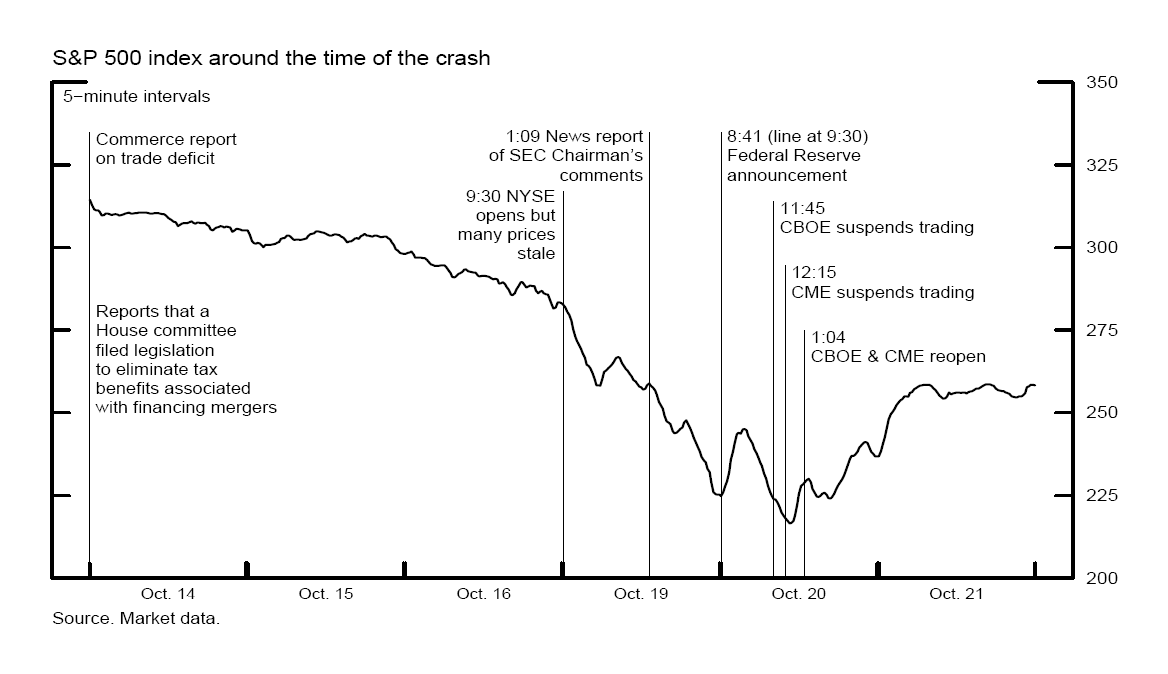
\includegraphics[height=0.36\textheight]{ch9_crash_1987.png}\\[1mm]
\imgcap{The S\&P 500 around 19 October 1987}
\imgcredit{https://commons.wikimedia.org/wiki/File:S\%26P_500_index_around_the_time_of_the_crash.png}{Figure: Mark Carlson, Federal Reserve Board (2006); public domain; Wikimedia Commons}
\end{column}
\begin{column}{0.56\textwidth}
\begin{itemize}
    \item 1987: a one-day fall of about 20\% in US equities shows that the tail, not the variance, decides solvency
    \item 1996: the Basel Committee adopts VaR for market risk and a traffic-light backtest of its hits \refBCBS
    \item 1999--2002: VaR is not coherent; ES is \refADEH, \refAT
    \item 2011--2016: ES is not elicitable \refGn, but (VaR, ES) is jointly elicitable \refFZ
    \item FRTB: capital on ES 2.5\%, backtests on VaR 1\% and VaR 2.5\% \refMAR
\end{itemize}
\end{column}
\end{columns}
\end{frame}

\begin{frame}{Basel: the forecaster and the referee}
\itemsize{\small}
\begin{columns}[T]
\begin{column}{0.36\textwidth}
\centering
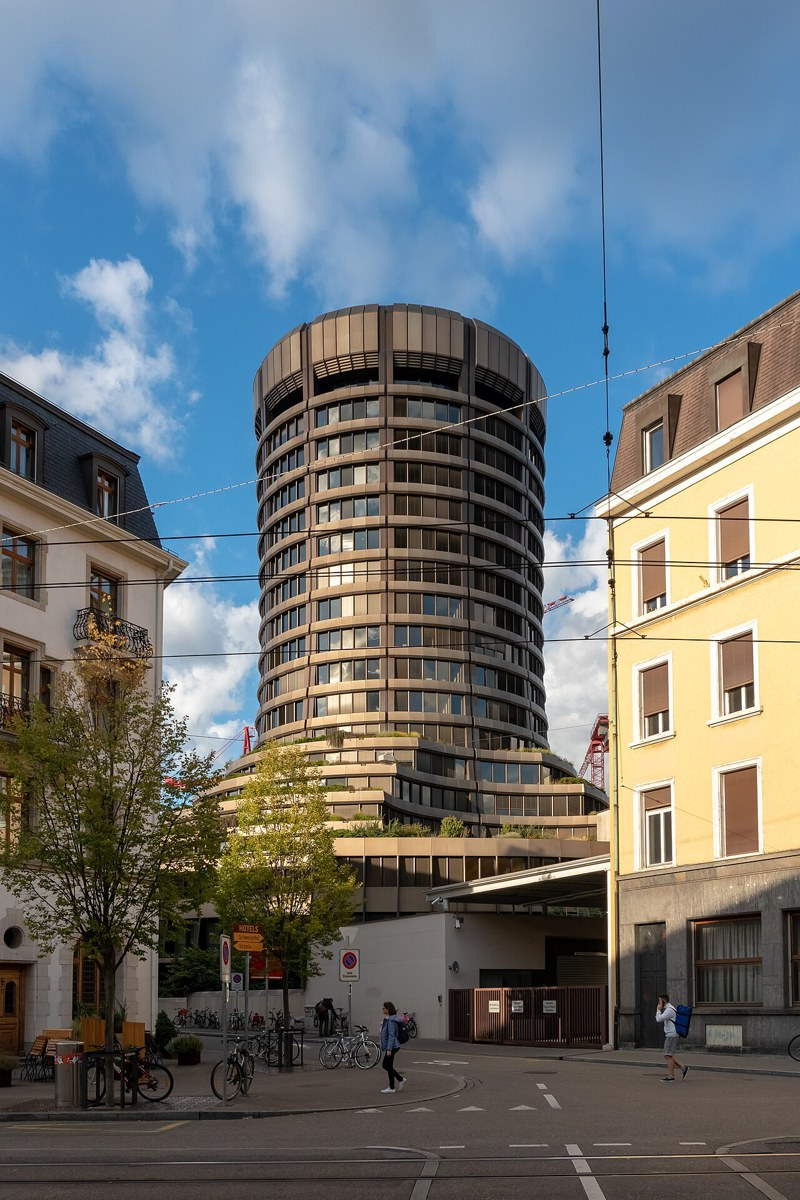
\includegraphics[height=0.5\textheight]{ch9_bis_basel_2018.jpg}\\[1mm]
\imgcap{Bank for International Settlements, Basel, 2018}
\imgcredit{https://commons.wikimedia.org/wiki/File:Bank_for_International_Settlements_in_the_late_afternoon.jpg}{Photo: Michal Pleskowicz (2018); CC BY-SA 4.0; Wikimedia Commons}
\end{column}
\begin{column}{0.62\textwidth}
\begin{itemize}
    \item A bank issues a daily forecast of its own tail; the supervisor checks it after the fact
    \item Two questions that statistics separates: is the forecast \textbf{calibrated} (backtest) and is it \textbf{better} than another (comparison)?
    \item Elicitability decides which forecasts can be compared at all \refNZ
    \item The incentive matters: a scoring rule rewards honest reporting only if it is strictly consistent for the target
\end{itemize}
\end{column}
\end{columns}
\end{frame}


%=============================================================================
\section{Risk measures as forecast functionals}
%=============================================================================

\begin{frame}{Known from TSA and MFM, and new here}
\itemsize{\small}
\begin{itemize}
    \item Known: VaR and ES by historical simulation, parametric, filtered HS and EVT; Kupiec and Christoffersen tests; the Basel traffic light (\atschlink{https://danpele.github.io/Time-Series-Analysis/EN/Courses/chapter5_conditional_volatility_garch.pdf}{TSA, Chapter 5}; MFM, Chapters 7--8)
    \item New: the forecasting view
    \begin{itemize}
        \item which losses are consistent for a quantile and for (VaR, ES); what elicitability buys and what it does not
        \item M-estimation of dynamic quantile and ES models: identification, asymptotics, non-smooth objectives
        \item backtests as moment tests of conditional calibration, with estimation risk; comparisons that survive multiple testing
    \end{itemize}
    \item Replications: Engle and Manganelli (2004) and Patton, Ziegel and Chen (2019), with the specifications of the papers, on our data
\end{itemize}
\end{frame}

\begin{frame}{VaR and ES as functionals (1/2): definitions}
\itemsize{\small}
\begin{itemize}
    \item VaR is minus a quantile of the return distribution
    \[ q_\alpha(F) = \inf\{y: F(y) \ge \alpha\}, \qquad \mathrm{VaR}_\alpha(F) = -q_\alpha(F) \]
    \begin{itemize}
        \item $Y$: the return, with distribution function $F$; $\alpha$: the level, i.e.\ the target hit rate (VaR 1\%: $\alpha = 0.01$)
        \item $q_\alpha(F)$: the smallest $y$ with $F(y) \ge \alpha$; a correct VaR is exceeded with probability $\Pr(Y < -\mathrm{VaR}_\alpha) = \alpha$
    \end{itemize}
    \item ES is minus the average of the quantiles below level $\alpha$ \refAT
    \[ \mathrm{ES}_\alpha(F) = -\frac{1}{\alpha}\int_0^\alpha q_u(F)\,du \]
    \begin{itemize}
        \item for continuous $F$: $\mathrm{ES}_\alpha = -\E[Y \mid Y \le q_\alpha]$, minus the mean return on the worst $\alpha$ share of days
        \item ES is coherent (subadditive) \refADEH; VaR is not; ES needs $\E|Y| < \infty$
    \end{itemize}
\end{itemize}
\end{frame}

\begin{frame}{VaR and ES as functionals (2/2): conventions}
\itemsize{\small}
\begin{itemize}
    \item In formulas we work on the return scale with the pair $(v, e) = (q_\alpha, -\mathrm{ES}_\alpha)$
    \begin{itemize}
        \item $v$: the $\alpha$-quantile of returns; $e$: the mean return beyond it; for the usual levels both are negative and $e \le v < 0$
    \end{itemize}
    \item Both are \textbf{functionals} $\mathrm T(F)$: maps from a distribution to a number
    \begin{itemize}
        \item a forecast of them is a point forecast of the predictive distribution, as in \atschlink{https://danpele.github.io/Advanced-Time-Series/EN/Courses/chapter1_forecast_evaluation.pdf}{Chapter 1}
    \end{itemize}
\end{itemize}
\end{frame}

\begin{frame}{Conditional risk forecasts: three routes (1/2)}
\itemsize{\small}
\begin{itemize}
    \item Target: the functional of the conditional distribution
    \[ (v_t, e_t) = \mathrm T(F_{t|t-1}) \]
    \begin{itemize}
        \item $F_{t|t-1}$: distribution of the return $Y_t$ given $\mathcal F_{t-1}$, the information up to day $t-1$
    \end{itemize}
    \item \textbf{Location--scale}: the return is a mean plus a volatility times an i.i.d. shock
    \[ Y_t = \mu_t + \sigma_t\eta_t \ \Rightarrow\ v_t = \mu_t + \sigma_t\,q_\alpha(\eta), \qquad e_t = \mu_t + \sigma_t\,\E[\eta \mid \eta \le q_\alpha(\eta)] \]
    \begin{itemize}
        \item $\mu_t$, $\sigma_t$: conditional mean and volatility (ARMA, GARCH); $q_\alpha(\eta)$: quantile of the shock distribution
        \item GARCH with Normal, skewed-t \refHan\ or empirical (EDF) innovations; the ratio $e_t/v_t$ is constant over time when $\mu_t = 0$
    \end{itemize}
\end{itemize}
\end{frame}

\begin{frame}{Conditional risk forecasts: three routes (2/2)}
\itemsize{\small}
\begin{itemize}
    \item \textbf{Direct quantile dynamics} \refEM: $v_t = v(\mathcal F_{t-1}; \beta)$
    \begin{itemize}
        \item $v(\cdot; \beta)$: a recursion with parameters $\beta$, estimated by the quantile (pinball) loss, without a distribution
    \end{itemize}
    \item \textbf{Joint semiparametric}: $(v_t, e_t) = (v, e)(\mathcal F_{t-1}; \theta)$
    \begin{itemize}
        \item two recursions with parameters $\theta$, estimated by a Fissler--Ziegel loss \refPZC, \refDB
    \end{itemize}
    \item Every route produces a point forecast of a functional; the scoring function of the next section is what makes them comparable
\end{itemize}
\end{frame}

\begin{frame}{Thirty-six years of tail forecasts}
\itemsize{\footnotesize}
\begin{center}
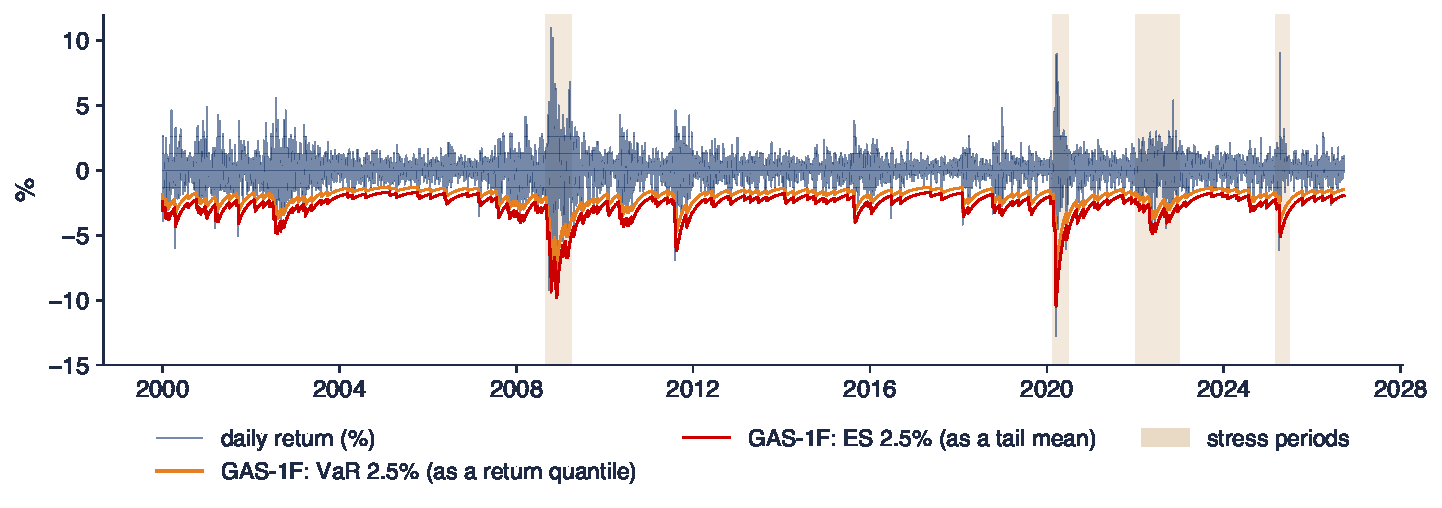
\includegraphics[width=0.97\textwidth,height=0.5\textheight,keepaspectratio]{ats_ch9_overview.pdf}
\end{center}
\vspace{-0.25cm}
\begin{itemize}
    \item S\&P 500 daily returns; the GAS-1F model of Patton, Ziegel and Chen, parameters estimated once on 1990--1999 and then only filtered; shaded: the four stress periods
\end{itemize}
\quantlet{ATS\_ch9\_pzc}{\qlurl{ATS_ch9_pzc}}
\end{frame}

\begin{frame}{Interpreting the long-run forecasts}
\itemsize{\small}
\begin{itemize}
    \item The ES 2.5\% forecast ranges from about \ensuremath{-}2.44\% (median) to \ensuremath{-}10.5\% on 17 March 2020: tail risk moves as much as volatility
    \item The forecasts react only on hit days and decay smoothly otherwise: the score-driven update of the GAS model
    \item Parameters fixed in 1999 still track 2008, 2020 and 2025: the dynamics generalise, the level does not need re-estimation
    \item Whether this is good enough is a testing question (Sections 5--6), not a visual one
\end{itemize}
\end{frame}

\begin{frame}{Recap: Risk measures as functionals}
\itemsize{\small}
\begin{itemize}
    \item VaR is a quantile, ES an integral of quantiles; both are functionals of the predictive distribution
    \item Three routes: location--scale, direct quantile dynamics, joint semiparametric models
    \item The convention: VaR 1\%, ES 2.5\%, $\alpha$ is the target hit rate
\end{itemize}
\end{frame}


%=============================================================================
\section{Elicitability and scoring functions}
%=============================================================================

\begin{frame}{Consistency, elicitability, identification (1/2)}
\itemsize{\small}
\begin{itemize}
    \item A scoring function $S(x, y)$ assigns a loss to the forecast $x$ when $y$ is observed; it is \textbf{consistent} for $\mathrm T$ on a class $\mathcal F$ if \refGn
    \[ \E_F S(\mathrm T(F), Y) \le \E_F S(x, Y) \quad \text{for all } x \text{ and } F \in \mathcal F \]
    \begin{itemize}
        \item $\E_F$: expectation when $Y \sim F$; the true functional value has the smallest expected loss
        \item \textbf{strictly} consistent: equality forces $x = \mathrm T(F)$; $\mathrm T$ is \textbf{elicitable} if a strictly consistent $S$ exists (\atschlink{https://danpele.github.io/Advanced-Time-Series/EN/Courses/chapter1_forecast_evaluation.pdf}{Chapter 1})
    \end{itemize}
\end{itemize}
\end{frame}

\begin{frame}{Consistency, elicitability, identification (2/2)}
\itemsize{\small}
\begin{itemize}
    \item \textbf{Identification function}: a function $V(x, y)$ whose mean is zero exactly at the true value
    \[ \E_F V(x, Y) = 0 \iff x = \mathrm T(F) \]
    \begin{itemize}
        \item quantile: $V(x, y) = \mathbf 1\{y \le x\} - \alpha$, with $\mathbf 1\{\cdot\}$ the indicator (1 if true, 0 otherwise); mean: $V(x, y) = x - y$
    \end{itemize}
    \item Osband's principle: the slope of the expected score is a positive multiple of the expected identification function \refFZ
    \[ \partial_x\E_F S(x, Y) = h(x)\,\E_F V(x, Y), \qquad h > 0 \]
    \begin{itemize}
        \item scores are integrated identification functions
    \end{itemize}
    \item Identification functions give \textbf{backtests} (is the forecast calibrated?); scoring functions give \textbf{comparisons} (which forecast is better?) \refNZ
\end{itemize}
\end{frame}

\begin{frame}{Quantiles: all consistent scores}
\itemsize{\small}
\begin{itemize}
    \item \textbf{Theorem} \refGn: under mild conditions, $S$ is consistent for $q_\alpha$ if and only if it is generalised piecewise linear (GPL)
    \[ S(x, y) = (\mathbf 1\{y \le x\} - \alpha)\big(G(x) - G(y)\big), \qquad G \text{ non-decreasing} \]
    \begin{itemize}
        \item $G(x) = x$: the pinball loss; $G$ strictly increasing gives strict consistency; $G(x) = \ln x$ for positive variables gives a scale-free (zero-homogeneous) score
        \item why: $\partial_x\E_F S(x, Y) = G'(x)\,(F(x) - \alpha)$, negative below $q_\alpha$, positive above (\atsapplink{atsapp1}{atssrc1}{Appendix})
    \end{itemize}
    \item Different $G$ give the same optimal forecast but can rank two misspecified forecasts differently: the choice of $G$ is a modelling choice
    \item Expectiles (asymmetric squared loss) are the only elicitable coherent risk measures \refZie; \refTayA\ uses them for VaR and ES
\end{itemize}
\end{frame}

\begin{frame}{ES is not elicitable}
\itemsize{\small}
\begin{itemize}
    \item \textbf{Necessary condition} \refGn: if $\mathrm T$ is elicitable, its level sets are convex
    \begin{itemize}
        \item level set: $\{F: \mathrm T(F) = t\}$, all distributions with the same functional value $t$; convex: closed under mixtures $\lambda F_0 + (1 - \lambda)F_1$, $\lambda \in [0, 1]$
        \item proof: if $\E_{F_0}S(t, Y) \le \E_{F_0}S(x, Y)$ and the same for $F_1$, the inequality holds for the mixture, because expectations are linear in $F$
    \end{itemize}
    \item Quantiles pass: if $F_0(t) = F_1(t) = \alpha$, then every mixture has $F_\lambda(t) = \alpha$
    \item ES fails: the mixture changes the quantile, so it changes which part of each component enters the tail mean \refWeb
    \begin{itemize}
        \item consequence: no loss function can rank ES forecasts alone; average losses of ES forecasts are not meaningful by themselves
    \end{itemize}
    \item Variance fails for the same reason; (mean, second moment) and (VaR, ES) are elicitable as pairs (\refFZ, ``higher order elicitability'')
\end{itemize}
\end{frame}

\begin{frame}{Level sets under mixing}
\itemsize{\footnotesize}
\begin{center}
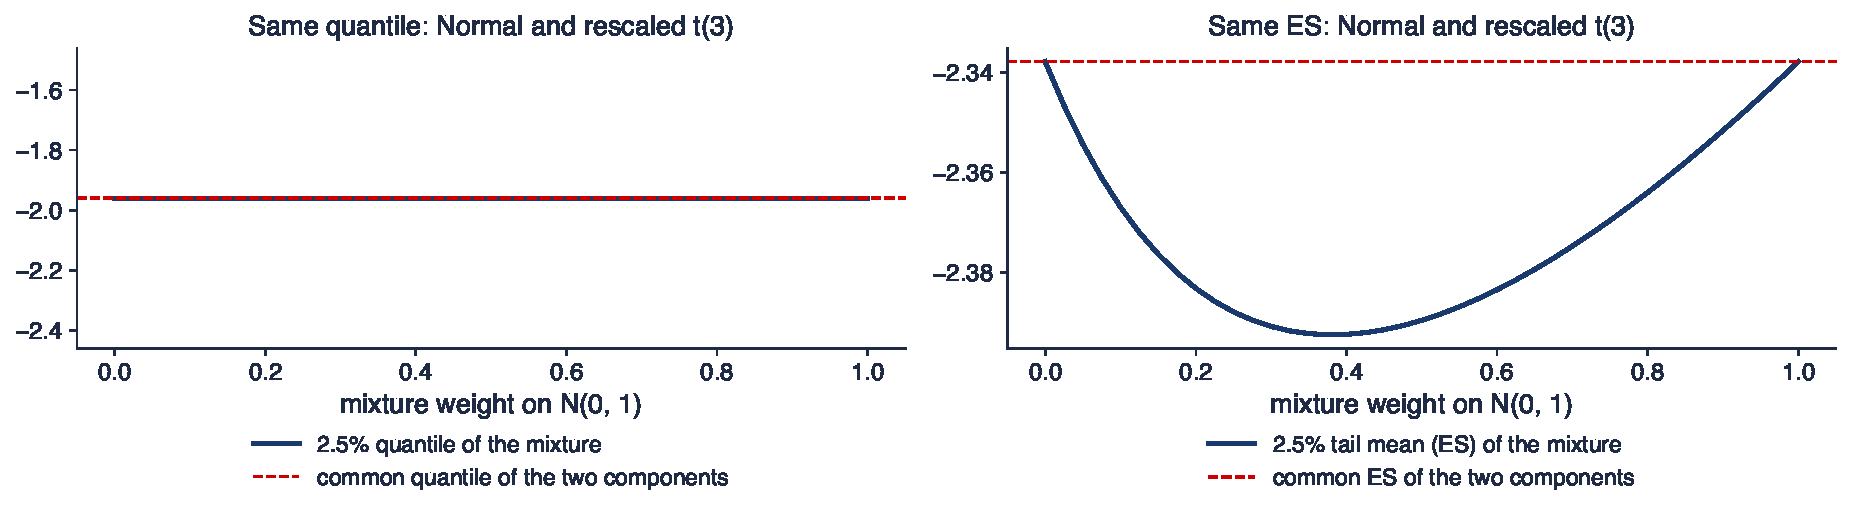
\includegraphics[width=0.97\textwidth,height=0.5\textheight,keepaspectratio]{ats_ch9_level_sets.pdf}
\end{center}
\vspace{-0.25cm}
\begin{itemize}
    \item Left: $N(0, 1)$ and a $t(3)$ rescaled to the same 2.5\% quantile; right: $N(0, 1)$ and a $t(3)$ rescaled to the same ES 2.5\%; curves: the functional of the mixture
\end{itemize}
\quantlet{ATS\_ch9\_scoring}{\qlurl{ATS_ch9_scoring}}
\end{frame}

\begin{frame}{Interpreting the level sets}
\itemsize{\small}
\begin{itemize}
    \item The quantile of every mixture stays at \ensuremath{-}1.96: the level set of $q_{0.025}$ is convex
    \item Both components have tail mean \ensuremath{-}2.338; the mixture moves away by up to 0.055 (at weight 0.38): the level set of ES is not convex
    \item The gap is small in numbers but decisive in logic: one counterexample rules out every strictly consistent loss for ES alone
    \item The way out is to forecast the quantile together with ES: the pair has a convex level set
\end{itemize}
\end{frame}

\begin{frame}{Joint elicitability: the Fissler--Ziegel class (1/2)}
\itemsize{\small}
\begin{itemize}
    \item \textbf{Theorem} \refFZ, in the form of \refPZC, eq.~(4): for $e \le v$, the loss
    \[ S(v, e, y) = (\mathbf 1\{y \le v\} - \alpha)\big(G_1(v) - G_1(y)\big) + G_2(e)\Big(v - e + \frac{1}{\alpha}\mathbf 1\{y \le v\}(y - v)\Big) - \mathcal G_2(e) \]
    \begin{itemize}
        \item is consistent for $(q_\alpha, -\mathrm{ES}_\alpha)$ if $G_1$ is non-decreasing and $G_2 = \mathcal G_2'$ is positive and increasing; strictly so under mild conditions
    \end{itemize}
    \item Reading the two parts
    \begin{itemize}
        \item first term: a GPL quantile score for $v$ (previous slides); $G_1$: any non-decreasing function
        \item second part: a Bregman-type score for $e$, evaluated against the tail mean implied by $v$; $\mathcal G_2$: an antiderivative of $G_2$
    \end{itemize}
\end{itemize}
\end{frame}

\begin{frame}{Joint elicitability: the Fissler--Ziegel class (2/2)}
\itemsize{\small}
\begin{itemize}
    \item Identification function of the pair: one component for the quantile, one for the tail mean
    \[ V_1 = \mathbf 1\{y \le v\} - \alpha, \qquad V_2 = e - v + \frac{1}{\alpha}\mathbf 1\{y \le v\}(v - y) \]
    \begin{itemize}
        \item $\E V_1 = 0$: $v$ is the $\alpha$-quantile; $\E V_2 = 0$ at the true quantile is the Acerbi--Tasche formula
        \item ES is the tail mean only together with the right quantile
    \end{itemize}
    \item Consequence \refFZG: ES can be \textbf{compared} through the pair; traditional ES backtests still need more than ES (Section 5)
\end{itemize}
\end{frame}

\begin{frame}{FZ0: the zero-homogeneous member}
\itemsize{\small}
\begin{itemize}
    \item \refPZC, Proposition 1: with $v, e < 0$, loss \textbf{differences} are invariant to rescaling $Y$ if and only if $G_1 = 0$ and $G_2(e) = -1/e$
    \[ L_{\mathrm{FZ0}}(y, v, e; \alpha) = -\frac{1}{\alpha e}\mathbf 1\{y \le v\}(v - y) + \frac{v}{e} + \ln(-e) - 1 \]
    \begin{itemize}
        \item first term: positive only on hit days ($y \le v$), proportional to the size of the hit; $v/e \in (0, 1]$; $\ln(-e)$ penalises an exaggerated ES
        \item the VaR part resembles the pinball loss; the ES part resembles QLIKE (\atschlink{https://danpele.github.io/Advanced-Time-Series/EN/Courses/chapter8_advanced_volatility.pdf}{Chapter 8})
    \end{itemize}
    \item Why zero homogeneity matters for time series
    \begin{itemize}
        \item with a non-homogeneous score, volatile days dominate the average loss and the DM test (heteroskedastic loss differences)
        \item FZ0 ranks forecasts in \% and in basis points identically; its value can be negative (EUR/RON)
        \item proof of consistency and of homogeneity: \atsapplink{atsapp2}{atssrc2}{Appendix}  % applink: FZ0, consistency and homogeneity
    \end{itemize}
    \item Iso-expected-loss contours are convex under mild conditions, which helps numerical minimisation \refPZC
\end{itemize}
\end{frame}

\begin{frame}{Expected losses around the truth}
\itemsize{\footnotesize}
\begin{center}
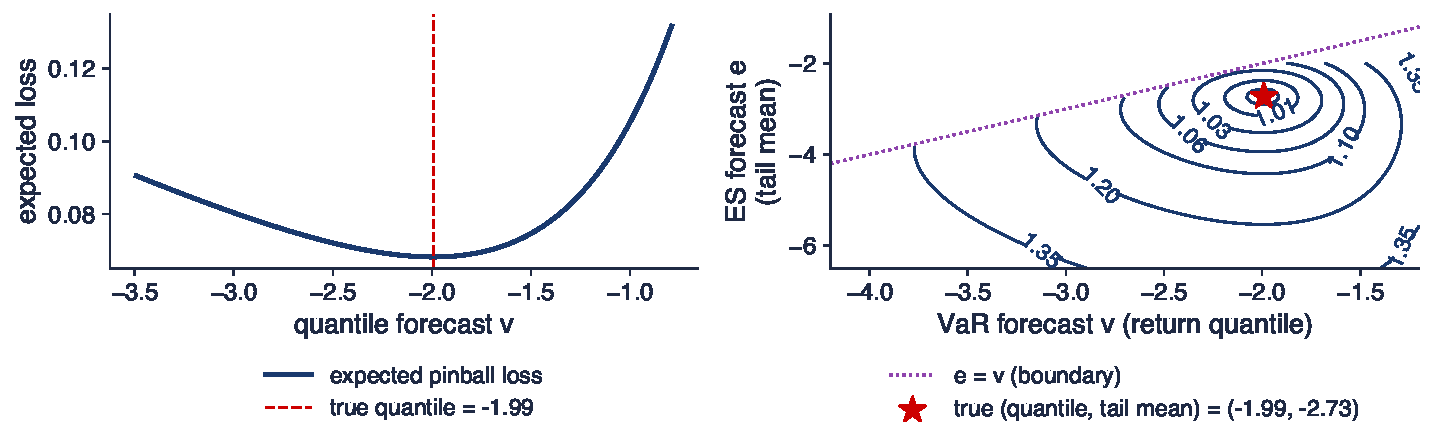
\includegraphics[width=0.97\textwidth,height=0.5\textheight,keepaspectratio]{ats_ch9_fz0_contour.pdf}
\end{center}
\vspace{-0.25cm}
\begin{itemize}
    \item Student $t(5)$ with unit variance, $\alpha = 0.025$, expectations by simulation ($4\times10^5$ draws): left, expected pinball loss; right, contours of the expected FZ0 loss
\end{itemize}
\quantlet{ATS\_ch9\_scoring}{\qlurl{ATS_ch9_scoring}}
\end{frame}

\begin{frame}{Interpreting the expected losses}
\itemsize{\small}
\begin{itemize}
    \item The pinball curve is minimal at \ensuremath{-}1.98, the true quantile \ensuremath{-}1.99: consistency in action
    \item The FZ0 surface is minimal at (\ensuremath{-}1.99, \ensuremath{-}2.73), minimum 1.004; contours are convex and elongated
    \item Both surfaces are flat near the optimum: large forecast differences cost little expected loss, so tests need many tail days
    \item Forecasts with $e > v$ are inadmissible: estimation must enforce the ordering
\end{itemize}
\end{frame}

\begin{frame}{Murphy diagrams: ranking for all consistent scores}
\itemsize{\small}
\begin{itemize}
    \item \refEGJK: every GPL quantile score is a mixture of \textbf{elementary scores}
    \[ S_\theta(x, y) = (\mathbf 1\{y < x\} - \alpha)\big(\mathbf 1\{\theta < x\} - \mathbf 1\{\theta < y\}\big), \qquad S(x, y) = \int S_\theta(x, y)\,dH(\theta) \]
    \begin{itemize}
        \item $\theta$: a threshold; $S_\theta$: the loss of a binary decision ``is the return below $\theta$?''; $H$: a non-decreasing weight over thresholds, corresponding to $G$
    \end{itemize}
    \item \textbf{Murphy diagram}: the average $\bar S_\theta$ of each forecast, plotted against $\theta$
    \begin{itemize}
        \item forecast A dominates B for every consistent score if and only if its curve is below for all $\theta$
        \item crossing curves: the ranking depends on $G$, i.e.\ on which thresholds the user cares about
    \end{itemize}
    \item A check on the pinball ranking that costs one line of code
\end{itemize}
\end{frame}

\begin{frame}{A Murphy diagram for VaR 2.5\%}
\itemsize{\footnotesize}
\begin{center}
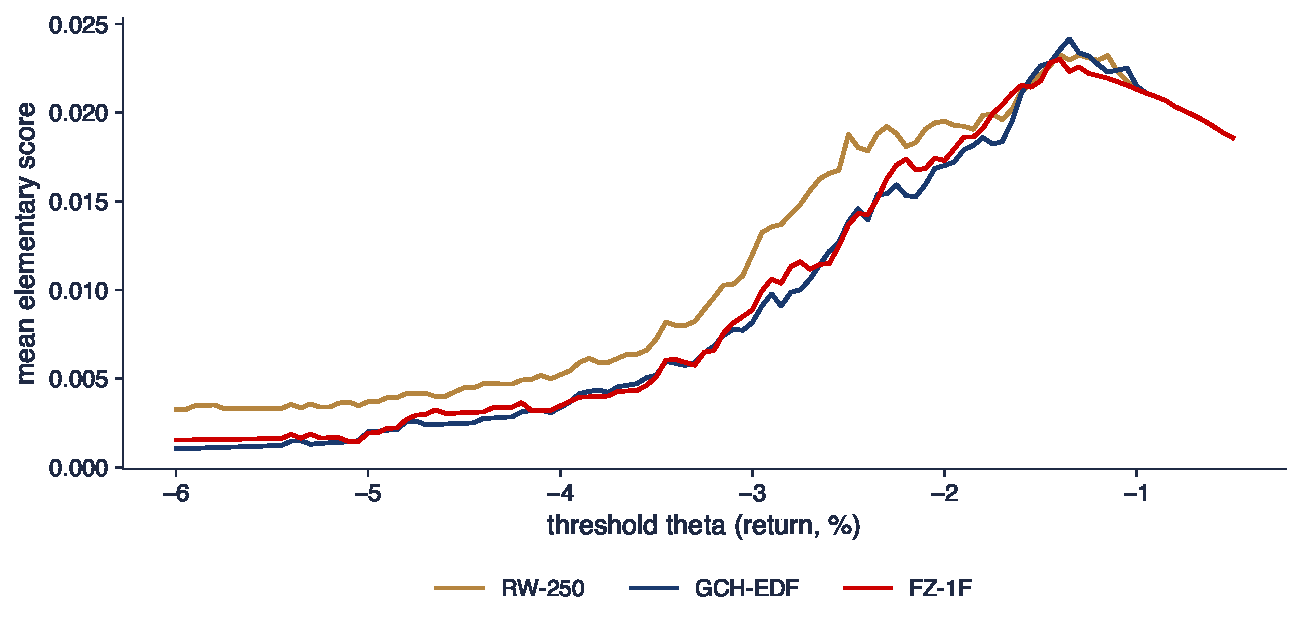
\includegraphics[width=0.97\textwidth,height=0.5\textheight,keepaspectratio]{ats_ch9_murphy.pdf}
\end{center}
\vspace{-0.25cm}
\begin{itemize}
    \item S\&P 500, out of sample 2000--2016 (PZC design); mean elementary scores of three VaR 2.5\% forecasts against the threshold $\theta$
\end{itemize}
\quantlet{ATS\_ch9\_scoring}{\qlurl{ATS_ch9_scoring}}
\end{frame}

\begin{frame}{Interpreting the Murphy diagram}
\itemsize{\small}
\begin{itemize}
    \item GARCH-EDF lies below RW-250 at 91\% of the thresholds: the dynamic forecast dominates almost uniformly
    \item GAS-1F and GARCH-EDF cross: GAS-1F is better at only 38\% of the thresholds; average pinball 7.66 and 7.45 ($\times 10^{-2}$)
    \item The two good models differ in deep thresholds (below $-4\%$), where data are scarce
    \item A claim that ``model A is better'' should say for which scores; the diagram answers it
\end{itemize}
\end{frame}

\begin{frame}{Recap: Elicitability}
\itemsize{\small}
\begin{itemize}
    \item Scores compare, identification functions test; both come from the same theory
    \item Quantiles: GPL scores; ES: not alone; (VaR, ES): the Fissler--Ziegel class
    \item FZ0 is scale-free; Murphy diagrams check rankings for all consistent scores
\end{itemize}
\end{frame}


%=============================================================================
\section{Quantile regression and CAViaR}
%=============================================================================

\begin{frame}{Quantile regression as M-estimation (1/2)}
\itemsize{\small}
\begin{columns}[T]
\begin{column}{0.27\textwidth}
\centering
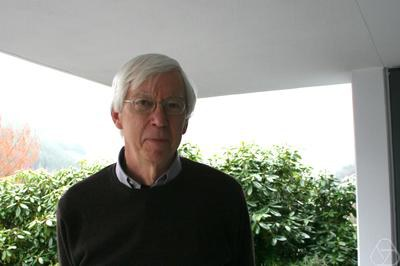
\includegraphics[height=0.26\textheight]{ch9_koenker_2012.jpg}\\[1mm]
\imgcap{Roger Koenker, Oberwolfach, 2012}
\imgcredit{https://commons.wikimedia.org/wiki/File:17224_Roger_W._Koenker.jpeg}{Photo: Ivonne Vetter, MFO (2012); CC BY-SA 2.0 de; Wikimedia Commons}
\end{column}
\begin{column}{0.71\textwidth}
\begin{itemize}
    \item \refKB: the $\alpha$-quantile of $y_t$ given $x_t$ is modelled as $x_t'\beta$ and estimated by minimising the pinball loss
    \[ \hat\beta(\alpha) = \arg\min_\beta \sum_t \rho_\alpha(y_t - x_t'\beta), \qquad \rho_\alpha(u) = u\,(\alpha - \mathbf 1\{u < 0\}) \]
    \begin{itemize}
        \item $x_t$: vector of regressors; $\rho_\alpha$: the check (pinball) function; the problem is a linear program
        \item $\rho_\alpha$ has slope $\alpha$ for positive residuals and $\alpha - 1$ for negative ones
        \item first-order condition: $\sum_t x_t(\mathbf 1\{y_t \le x_t'\hat\beta\} - \alpha) \approx 0$, the identification function
    \end{itemize}
\end{itemize}
\end{column}
\end{columns}
\end{frame}

\begin{frame}{Quantile regression as M-estimation (2/2)}
\itemsize{\small}
\begin{itemize}
    \item Asymptotic distribution \refKoe: a sandwich in which the density at the quantile appears
    \[ \sqrt T(\hat\beta - \beta) \to N\big(0, \alpha(1 - \alpha)D^{-1}\Omega D^{-1}\big), \qquad \Omega = \E[x_tx_t'], \qquad D = \E[f_t(q_t)x_tx_t'] \]
    \begin{itemize}
        \item $f_t(q_t)$: conditional density of $y_t$ at its true quantile $q_t$; its inverse is called the ``sparsity''
        \item few observations near the quantile (small $f_t$) mean an imprecise $\hat\beta$; $f_t$ is estimated with a kernel and a bandwidth
    \end{itemize}
    \item Time series: quantile autoregression \refKX\ lets AR coefficients vary across quantiles; CAViaR makes the quantile itself autoregressive
\end{itemize}
\end{frame}

\begin{frame}{CAViaR: the four specifications}
\itemsize{\footnotesize}
\begin{columns}[T]
\begin{column}{0.26\textwidth}
\centering
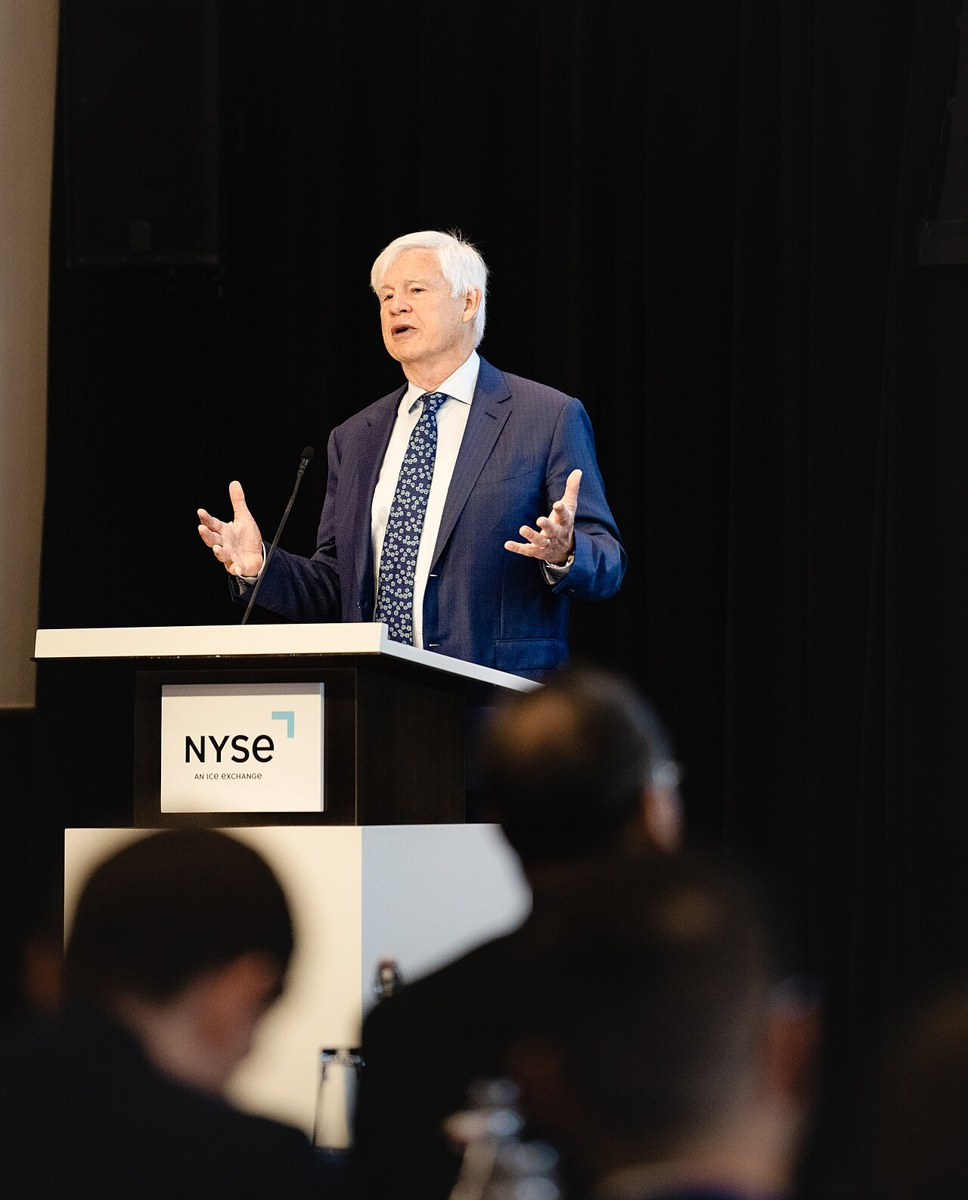
\includegraphics[height=0.32\textheight]{ch9_engle_2022.jpg}\\[1mm]
\imgcap{Robert Engle, 2022}
\imgcredit{https://commons.wikimedia.org/wiki/File:0603-Kraneshares_KRBN-RobertEngle-JonDemske-13.jpg}{Photo: Jon Demske (2022); CC BY-SA 4.0; Wikimedia Commons}
\end{column}
\begin{column}{0.72\textwidth}
\begin{itemize}
    \item \refEM, written for $\mathrm{VaR}_t = -q_t(\alpha) > 0$; $y_{t-1}$: yesterday's return; $\beta_j$: parameters:
    \item \textbf{SAV} (symmetric absolute value): $\mathrm{VaR}_t = \beta_1 + \beta_2\mathrm{VaR}_{t-1} + \beta_3|y_{t-1}|$
    \begin{itemize}
        \item $\beta_2$: the persistence of the tail; $\beta_3$: the reaction to the size of yesterday's return
    \end{itemize}
    \item \textbf{AS} (asymmetric slope): $\mathrm{VaR}_t = \beta_1 + \beta_2\mathrm{VaR}_{t-1} + \beta_3(y_{t-1})^+ + \beta_4(y_{t-1})^-$
    \begin{itemize}
        \item $(y)^+ = \max(y, 0)$, $(y)^- = -\min(y, 0)$: gains and losses enter separately; $\beta_4 > \beta_3$ is a leverage effect
    \end{itemize}
    \item \textbf{IG} (indirect GARCH): $\mathrm{VaR}_t = (\beta_1 + \beta_2\mathrm{VaR}_{t-1}^2 + \beta_3y_{t-1}^2)^{1/2}$, a GARCH(1,1) with i.i.d.\ innovations
    \item \textbf{Adaptive}: $\mathrm{VaR}_t = \mathrm{VaR}_{t-1} + \beta_1\big([1 + e^{G(y_{t-1} + \mathrm{VaR}_{t-1})}]^{-1} - \alpha\big)$
    \begin{itemize}
        \item the bracket is a smooth hit indicator ($G = 10$): VaR rises after a hit and falls slowly otherwise; no distribution is assumed in any of the four
    \end{itemize}
\end{itemize}
\end{column}
\end{columns}
\end{frame}

\begin{frame}{Estimation and inference (1/2): the criterion}
\itemsize{\small}
\begin{itemize}
    \item Regression-quantile criterion: the average pinball loss of the implied quantile path
    \[ \hat\beta = \arg\min_\beta \frac1T\sum_t \rho_\alpha\big(y_t + \mathrm{VaR}_t(\beta)\big) \]
    \begin{itemize}
        \item $\mathrm{VaR}_t(\beta)$: the path generated by the recursion with parameters $\beta$; the criterion is non-differentiable and non-convex in $\beta$
    \end{itemize}
    \item EM procedure (empirical section)
    \begin{itemize}
        \item $\mathrm{VaR}_1$: the empirical quantile of the first 300 days; $10^4$ random parameter vectors, the 10 best refined by alternating simplex and quasi-Newton steps
    \end{itemize}
\end{itemize}
\end{frame}

\begin{frame}{Estimation and inference (2/2): the covariance}
\itemsize{\small}
\begin{itemize}
    \item Consistency and asymptotic normality, with a sandwich covariance
    \[ \sqrt T(\hat\beta - \beta) \to N\big(0, \alpha(1 - \alpha)D^{-1}AD^{-1}\big), \qquad A = \E[\nabla q_t\nabla q_t'], \qquad D = \E[f_t(q_t)\nabla q_t\nabla q_t'] \]
    \begin{itemize}
        \item $\nabla q_t = \partial q_t(\beta)/\partial\beta$: gradient of the quantile path, which follows its own recursion (or numerical differentiation of the path)
        \item $f_t(q_t)$: conditional density of $y_t$ at the quantile, as in quantile regression
    \end{itemize}
    \item Estimator of $D$: count the residuals within $\hat c$ of zero
    \[ \hat D = \frac{1}{2T\hat c}\sum_t\mathbf 1\{|y_t - \hat q_t| < \hat c\}\,\nabla\hat q_t\nabla\hat q_t' \]
    \begin{itemize}
        \item $\hat c$: bandwidth, from the Hall--Sheather rule on the residual scale \refKoe; the dynamic model is a recursive M-estimator
    \end{itemize}
\end{itemize}
\end{frame}

\begin{frame}{The dynamic quantile (DQ) test}
\itemsize{\footnotesize}
\begin{itemize}
    \item The hit sequence is a martingale difference under correct specification
    \[ \mathrm{Hit}_t = \mathbf 1\{y_t < q_t\} - \alpha, \qquad \E[\mathrm{Hit}_t \mid \mathcal F_{t-1}] = 0 \]
    \begin{itemize}
        \item regress $\mathrm{Hit}_t$ on $X_t$ = (1, $\mathrm{Hit}_{t-1}, \dots, \mathrm{Hit}_{t-4}$, $q_t$), all in $\mathcal F_{t-1}$ \refEM
    \end{itemize}
    \item Out-of-sample statistic: a Wald test that all regression coefficients are zero
    \[ \mathrm{DQ} = \frac{\mathrm{Hit}'X(X'X)^{-1}X'\mathrm{Hit}}{\alpha(1 - \alpha)} \to \chi^2_6 \]
    \begin{itemize}
        \item $\mathrm{Hit}$: vector of hits; $X$: matrix with rows $X_t$; 6 = number of regressors; a large DQ rejects calibration
        \item in sample the estimated $\beta$ makes the hits orthogonal to the gradients: the covariance needs the correction derived by EM
    \end{itemize}
    \item Kupiec (constant only) and Christoffersen (the first lag of the hits) are special cases; the VaR regressor adds power against level-dependent misspecification
    \item With $\alpha = 1\%$ and a few hundred days the $\chi^2$ approximation is poor (Section 5): report simulated or exact p-values when possible
\end{itemize}
\end{frame}

\begin{frame}{Case study: Engle and Manganelli (2004) on today's data}
\itemsize{\small}
\begin{itemize}
    \item The design of the empirical section of EM: 3,392 daily returns, the first 2,892 for estimation, the last 500 out of sample; VaR 1\% and 5\%
    \begin{itemize}
        \item EM used 1986--1999 (GM, IBM, S\&P 500); we use the S\&P 500 from 25 March 2013 to 18 September 2026, out of sample from 20 September 2024
    \end{itemize}
    \item Same specifications, starting values and search; the April 2025 tariff shock falls in the out-of-sample period
    \item Questions: which specification fits the 1\% tail, are the forecasts calibrated out of sample, and is the response to bad news asymmetric?
\end{itemize}
\end{frame}

\begin{frame}{CAViaR VaR 1\% of the S\&P 500}
\itemsize{\footnotesize}
\begin{center}
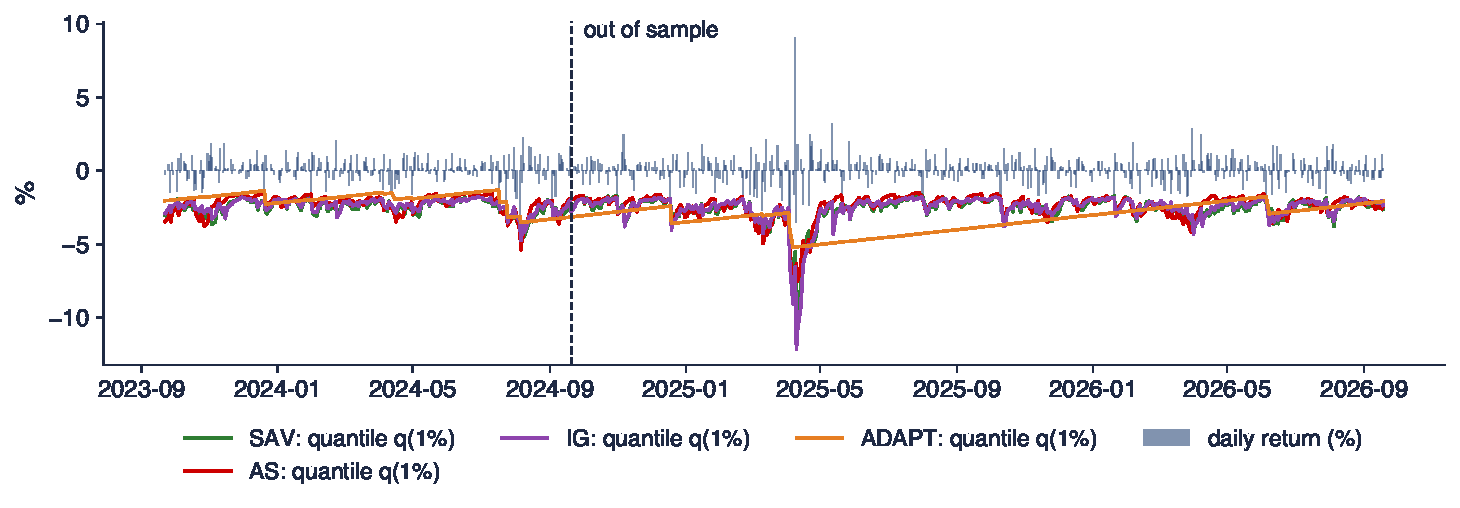
\includegraphics[width=0.97\textwidth,height=0.5\textheight,keepaspectratio]{ats_ch9_caviar.pdf}
\end{center}
\vspace{-0.25cm}
\begin{itemize}
    \item The last year of the estimation sample and the 500 out-of-sample days; lines: the 1\% return quantile $q_t = -\mathrm{VaR}_t$ of the four specifications
\end{itemize}
\quantlet{ATS\_ch9\_caviar}{\qlurl{ATS_ch9_caviar}}
\end{frame}

\begin{frame}{Estimates, standard errors and DQ tests}
\itemsize{\footnotesize}
\setlength{\tabcolsep}{3pt}
\begin{center}
\scriptsize
\begin{tabular}{lrrrrrrrr}
\toprule
\textbf{Model} & $\beta_1$ & $\beta_2$ & $\beta_3$ & $\beta_4$ & RQ$\times10^2$ & \shortstack[r]{hits in\\sample (\%)} & \shortstack[r]{hits out of\\sample (\%)} & \shortstack[r]{DQ out of\\sample ($p$)} \\
\midrule
SAV & 0.359 (0.217) & 0.702 (0.118) & 0.604 (0.243) & -- & 3.305 & 1.0 & 1.4 & 14.4 (0.025) \\
AS & 0.264 (0.137) & 0.805 (0.080) & 0.044 (0.185) & 0.616 (0.149) & 3.220 & 1.0 & 1.2 & 15.8 (0.015) \\
IG & 0.942 (0.467) & 0.674 (0.105) & 1.429 (0.702) & -- & 3.267 & 1.0 & 1.2 & 2.3 (0.891) \\
ADAPT & 1.190 (0.069) & -- & -- & -- & 4.044 & 0.9 & 0.8 & 27.5 ($<$0.001) \\
\bottomrule
\end{tabular}
\end{center}
\begin{itemize}
    \item Standard errors from the asymptotic covariance of EM; RQ: the minimised in-sample criterion; DQ out of sample with four lagged hits and the VaR, $\chi^2_6$; 500 days give 5 expected hits
    \item Out-of-sample average pinball loss ($\times10^2$): SAV 3.87, AS 3.66, IG 3.66, adaptive 4.42
\end{itemize}
\end{frame}

\begin{frame}{Interpreting the CAViaR estimates}
\itemsize{\small}
\begin{itemize}
    \item All three autoregressive models fit the in-sample rate (about 1\%) by construction: the quantile loss calibrates the level
    \item AS: a negative return moves VaR about 14 times more than a positive one of the same size; $\beta_3$ is not distinguishable from zero
    \item Out of sample IG passes DQ ($p$ = 0.891); SAV ($p$ = 0.025) and AS ($p$ = 0.015) are rejected at 5\%, the adaptive model clearly ($p$ $<$0.001)
    \item Five expected hits in 500 days: rejections come from clustered hits in April 2025, not from the count; such evidence is fragile
    \item The adaptive model reacts only to hits, like a slow thermostat: after the April 2025 cluster it stays too high for months
\end{itemize}
\end{frame}

\begin{frame}{News impact curves}
\itemsize{\footnotesize}
\begin{center}
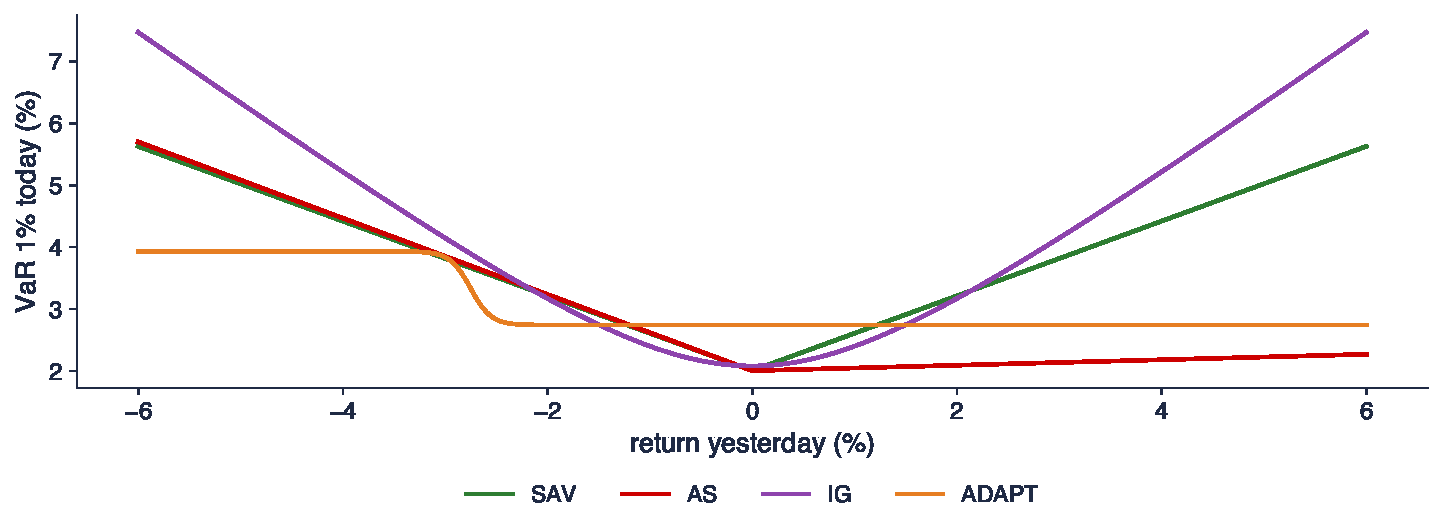
\includegraphics[width=0.97\textwidth,height=0.5\textheight,keepaspectratio]{ats_ch9_nic.pdf}
\end{center}
\vspace{-0.25cm}
\begin{itemize}
    \item $\mathrm{VaR}_t$ as a function of $y_{t-1}$, with $\mathrm{VaR}_{t-1}$ at its in-sample median (2.16\% for AS); estimated parameters of the table
\end{itemize}
\quantlet{ATS\_ch9\_caviar}{\qlurl{ATS_ch9_caviar}}
\end{frame}

\begin{frame}{Interpreting the news impact curves}
\itemsize{\small}
\begin{itemize}
    \item SAV and IG are symmetric by design: a 5\% rally raises the 1\% VaR as much as a 5\% fall
    \item AS is almost flat for gains and steep for losses: the leverage effect estimated directly in the tail
    \item The adaptive curve is a step: only the sign of the hit matters, not its size
    \item The shape of the curve is a testable restriction: AS nests SAV ($\beta_3 = \beta_4$), a Wald test with the asymptotic covariance of EM
\end{itemize}
\end{frame}

\begin{frame}{Recap: CAViaR}
\itemsize{\small}
\begin{itemize}
    \item Quantile regression is M-estimation with the pinball loss; its covariance needs the density at the quantile
    \item CAViaR makes the quantile autoregressive; estimation needs many starts
    \item DQ tests hits against information; the asymmetric model fits equity tails
\end{itemize}
\end{frame}


%=============================================================================
\section{Semiparametric models for (VaR, ES)}
%=============================================================================

\begin{frame}{M-estimation with the FZ0 loss}
\itemsize{\small}
\begin{itemize}
    \item A dynamic model for the pair, estimated by minimising the average FZ0 loss \refPZC
    \[ (v_t, e_t) = (v, e)(\mathcal F_{t-1}; \theta), \qquad \hat\theta = \arg\min_\theta \frac1T\sum_t L_{\mathrm{FZ0}}\big(y_t, v_t(\theta), e_t(\theta); \alpha\big) \]
    \begin{itemize}
        \item $\theta$: parameters of the two recursions; consistency follows from the strict consistency of FZ0 and the identification of $\theta$
        \item asymptotic normality as for CAViaR, with a sandwich covariance
    \end{itemize}
    \item Why not maximum likelihood?
    \begin{itemize}
        \item MLE needs the whole distribution; a wrong body or right tail distorts the left tail estimates
        \item FZ estimation targets exactly the two tail functionals: less efficient if the model is right, robust if it is not (PZC, Tables 3--4)
    \end{itemize}
    \item Related: the asymmetric Laplace quasi-likelihood \refTayB; ES regressions \refDB; score-driven (GAS) dynamics \refCKL
\end{itemize}
\end{frame}

\begin{frame}{The two-factor GAS model}
\itemsize{\small}
\begin{itemize}
    \item \refPZC, eq.~(9)--(16): the pair follows a VAR(1) driven by the scaled score of FZ0 (generalised autoregressive score, GAS)
    \[ \begin{pmatrix} v_{t+1} \\ e_{t+1}\end{pmatrix} = w + B\begin{pmatrix} v_t \\ e_t\end{pmatrix} + A\lambda_t \]
    \begin{itemize}
        \item $w$: intercept vector; $B$: diagonal $2\times2$ persistence matrix; $A$: $2\times2$ matrix of reactions to the forcing variables $\lambda_t = (\lambda_{v,t}, \lambda_{e,t})'$
    \end{itemize}
    \item Forcing variables from the FZ0 score
    \[ \lambda_{v,t} = -v_t\big(\mathbf 1\{y_t \le v_t\} - \alpha\big), \qquad \lambda_{e,t} = \frac{1}{\alpha}\mathbf 1\{y_t \le v_t\}\,y_t - e_t \]
    \begin{itemize}
        \item both are identification functions: zero conditional mean under correct specification
        \item the Hessian is scaled with $f_t(v_t) \approx k_\alpha/v_t$, $k_\alpha$ a constant (exact for location--scale returns), so no density is estimated
        \item eight parameters; on non-hit days $\lambda_{e,t} = -e_t$ and both risk measures decay deterministically towards their means
    \end{itemize}
\end{itemize}
\end{frame}

\begin{frame}{One-factor, GARCH-FZ and Hybrid models}
\itemsize{\footnotesize}
\begin{itemize}
    \item \textbf{GAS-1F}, eq.~(20): one latent log-scale $\kappa_t$ multiplies both risk measures
    \[ v_t = a\,e^{\kappa_t}, \quad e_t = b\,e^{\kappa_t}, \quad \kappa_t = \beta\kappa_{t-1} + \gamma\,\frac{-1}{e_{t-1}}\Big(\frac{1}{\alpha}\mathbf 1\{y_{t-1} \le v_{t-1}\}y_{t-1} - e_{t-1}\Big) \]
    \begin{itemize}
        \item $b < a < 0$: VaR and ES at $\kappa_t = 0$; $\beta$: persistence of the log-scale; $\gamma$: reaction to the ES forcing variable
        \item the intercept $\omega$ is not identified together with $(a, b)$ and is fixed at 0
    \end{itemize}
    \item \textbf{GARCH-FZ}, eq.~(25)--(26): $\kappa_t^2 = 1 + \beta\kappa_{t-1}^2 + \gamma y_{t-1}^2$, $(v_t, e_t) = (a, b)\kappa_t$: a GARCH whose scale $\kappa_t$ is fitted to the tail
    \item \textbf{Hybrid}, eq.~(27): GAS-1F plus $\delta\ln|y_{t-1}|$ in the recursion of $\kappa_t$
    \begin{itemize}
        \item reacts every day through $\delta$, more strongly on hit days
    \end{itemize}
    \item In all three the ratio $e_t/v_t = b/a$ is constant: the shape of the tail is fixed, only its scale moves
\end{itemize}
\end{frame}

\begin{frame}{Estimating non-smooth recursive models}
\itemsize{\small}
\begin{itemize}
    \item The FZ0 objective is discontinuous in $\theta$ (through $\mathbf 1\{y_t \le v_t(\theta)\}$) and the recursion propagates every jump
    \item Appendix C of the paper \refPZC: replace the indicator by a logistic approximation in the loss and in the forcing variable
    \[ \Gamma(y, v; \tau) = \frac{1}{1 + e^{\tau(y - v)}} \]
    \begin{itemize}
        \item $\tau > 0$: smoothing parameter; as $\tau \to \infty$, $\Gamma \to \mathbf 1\{y \le v\}$
        \item quasi-Newton with $\tau = 5$, then $\tau = 20$, then the exact loss with the simplex method, each step starting from the previous one
    \end{itemize}
    \item Our starting values: random dynamic parameters with $(a, b)$ matched to the in-sample VaR and ES; the four best are refined
    \item Constraints enforced by penalty: $e_t \le v_t$, $e_t < 0$, stationarity of the recursion
\end{itemize}
\end{frame}

\begin{frame}{Case study: Patton, Ziegel and Chen (2019), Section 5}
\itemsize{\small}
\begin{itemize}
    \item Data: daily S\&P 500 returns, January 1990 -- December 2016; estimation on the first ten years, parameters kept fixed for 2000--2016 ($T = 4\,275$)
    \item Ten models, as in the paper
    \begin{itemize}
        \item rolling windows of 125, 250 and 500 days (RW); ARMA (order by BIC) -- GARCH(1,1) with Normal, skewed-t or empirical innovations
        \item GAS-2F, GAS-1F, GARCH-FZ and Hybrid estimated by FZ0 minimisation
    \end{itemize}
    \item Outputs replicated: average out-of-sample FZ0 losses (Table 8, $\alpha$ = 5\%; Table S5, $\alpha$ = 2.5\%), DM statistics (Table 9), goodness-of-fit tests (eq.~41)
    \item Our data: EODHD closes of the same index; differences of a few thousandths are expected from data revisions and optimiser paths
\end{itemize}
\end{frame}

\begin{frame}{Three ways to forecast the tail}
\itemsize{\footnotesize}
\begin{center}
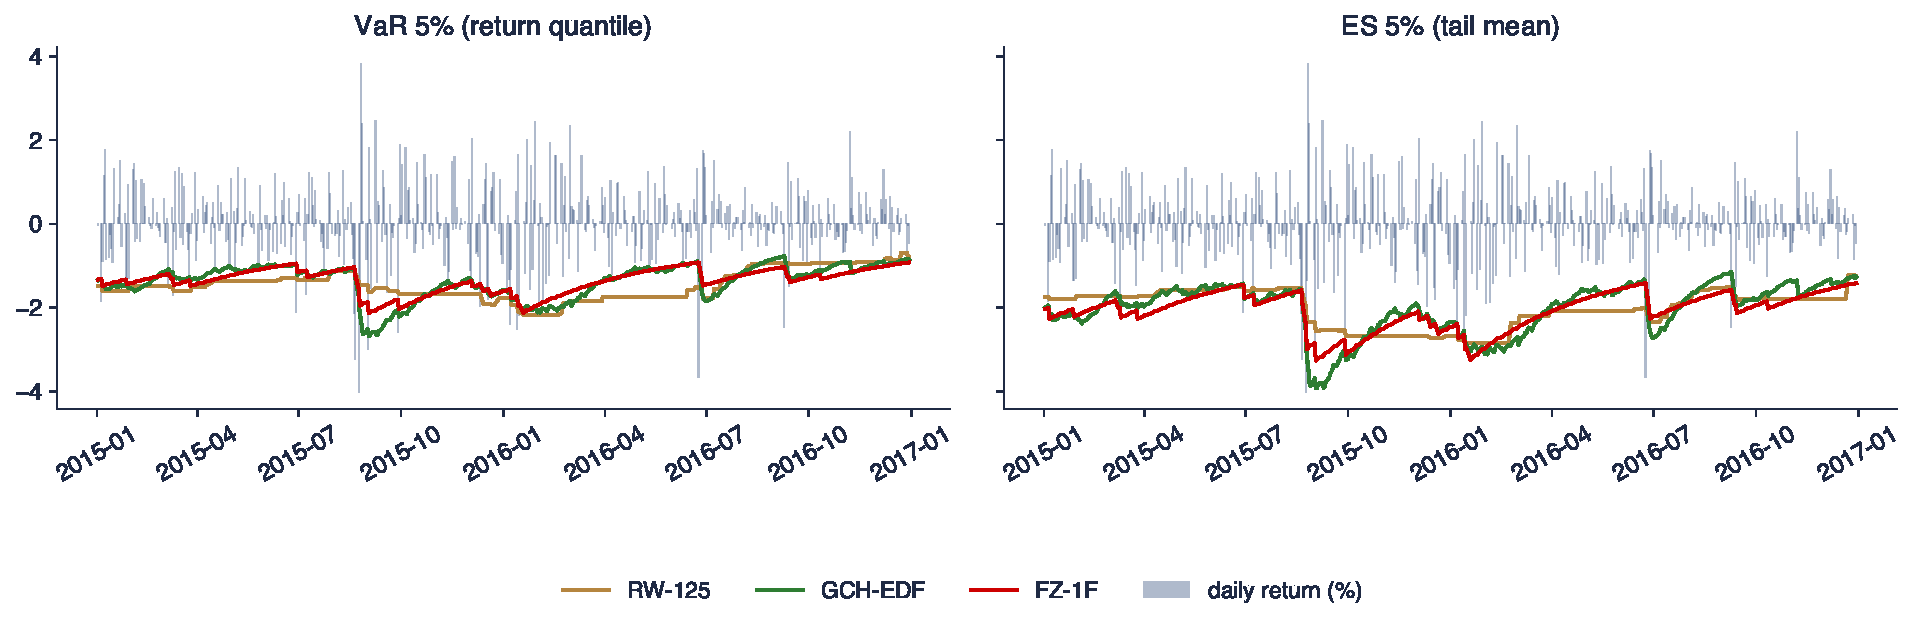
\includegraphics[width=0.97\textwidth,height=0.5\textheight,keepaspectratio]{ats_ch9_pzc_paths.pdf}
\end{center}
\vspace{-0.25cm}
\begin{itemize}
    \item VaR and ES 5\% of the S\&P 500 in 2015--2016 (PZC, Figure 5 on our data): RW-125, GARCH-EDF and GAS-1F
\end{itemize}
\quantlet{ATS\_ch9\_pzc}{\qlurl{ATS_ch9_pzc}}
\end{frame}

\begin{frame}{Interpreting the three forecasts}
\itemsize{\small}
\begin{itemize}
    \item The rolling window moves in steps as extreme days enter and leave the window, months after the shock
    \item GARCH-EDF moves every day with squared returns; GAS-1F moves only on hit days and then decays smoothly
    \item August 2015: GARCH reacts most, GAS-1F jumps less but stays; in 2008 the GAS-1F ES 5\% reached \ensuremath{-}9.9\%
    \item Which reaction is right is decided by the FZ0 loss, not by the look of the path
\end{itemize}
\end{frame}

\begin{frame}{Replication: average out-of-sample FZ0 loss}
\itemsize{\footnotesize}
\begin{center}
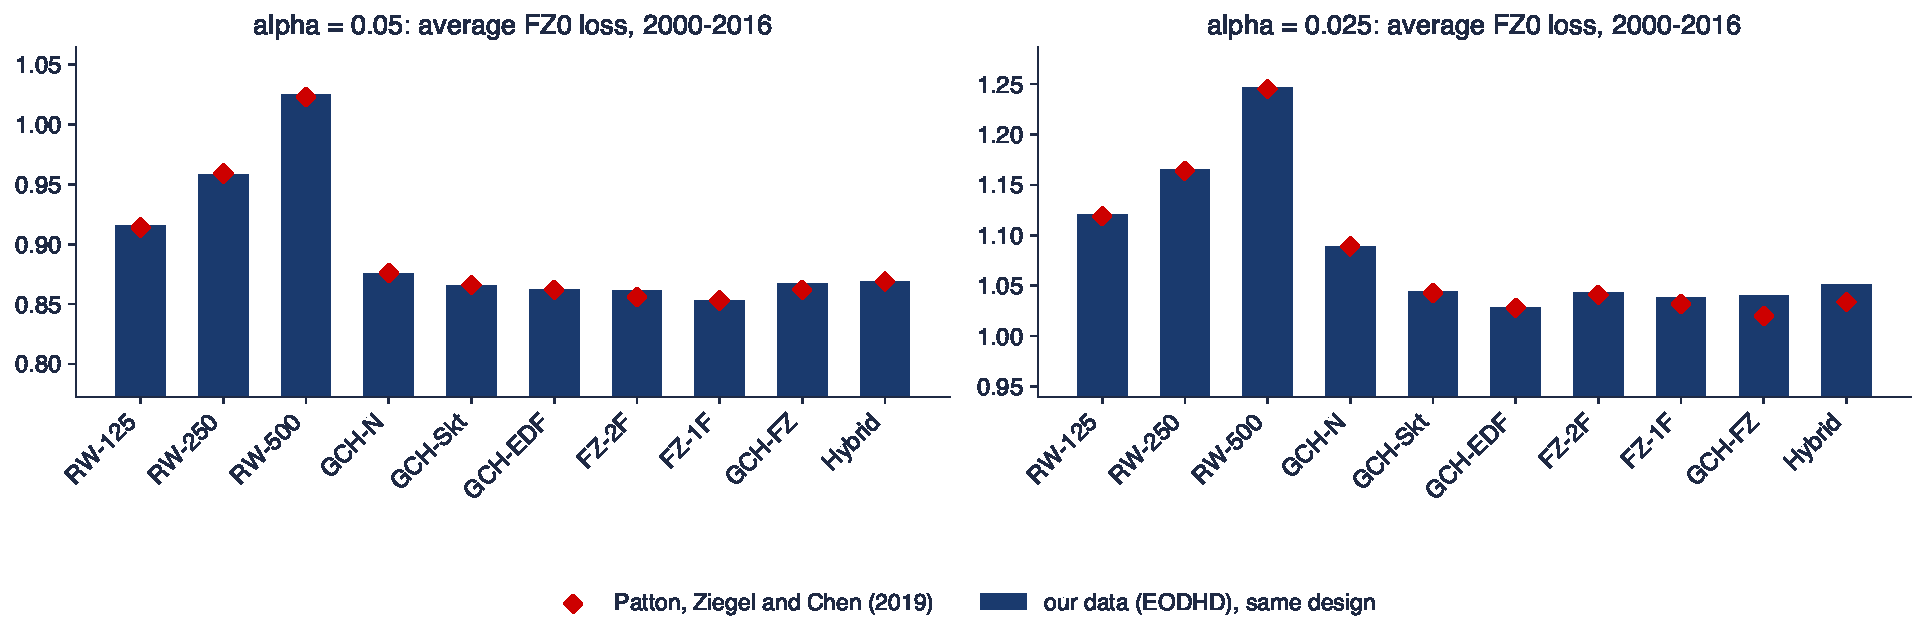
\includegraphics[width=0.97\textwidth,height=0.5\textheight,keepaspectratio]{ats_ch9_pzc_table.pdf}
\end{center}
\vspace{-0.25cm}
\begin{itemize}
    \item Bars: our data and code, same design; diamonds: the values printed in PZC, Table 8 ($\alpha$ = 5\%) and Table S5 ($\alpha$ = 2.5\%)
\end{itemize}
\quantlet{ATS\_ch9\_pzc}{\qlurl{ATS_ch9_pzc}}
\end{frame}

\begin{frame}{Replication in numbers}
\itemsize{\footnotesize}
\begin{center}
\scriptsize
\begin{tabular}{lcccccc}
\toprule
\textbf{Model} & \multicolumn{2}{c}{$\alpha = 5\%$} & \multicolumn{2}{c}{$\alpha = 2.5\%$} & \multicolumn{2}{c}{GoF $p$, $\alpha = 5\%$} \\ & ours & PZC & ours & PZC & VaR & ES \\
\midrule
RW-125 & 0.916 & 0.914 & 1.120 & 1.119 & 0.004 & 0.005 \\
RW-250 & 0.959 & 0.959 & 1.165 & 1.164 & $<$0.001 & 0.011 \\
RW-500 & 1.025 & 1.023 & 1.247 & 1.245 & $<$0.001 & $<$0.001 \\
GCH-N & 0.876 & 0.876 & 1.089 & 1.089 & 0.018 & $<$0.001 \\
GCH-Skt & 0.865 & 0.866 & 1.044 & 1.043 & 0.001 & 0.001 \\
GCH-EDF & 0.862 & 0.862 & 1.028 & 1.028 & 0.001 & 0.007 \\
FZ-2F & 0.862 & 0.856 & 1.044 & 1.041 & $<$0.001 & 0.003 \\
FZ-1F & 0.853 & 0.853 & 1.038 & 1.032 & 0.001 & 0.037 \\
GCH-FZ & 0.867 & 0.862 & 1.040 & 1.020 & 0.005 & 0.016 \\
Hybrid & 0.869 & 0.869 & 1.051 & 1.034 & $<$0.001 & $<$0.001 \\
\bottomrule
\end{tabular}
\end{center}
\begin{itemize}
    \item Largest gap: 0.006 at 5\%, 0.020 at 2.5\%; BIC picks ARMA(0, 0) for the mean (PZC: ARMA(1,1)); GARCH $\alpha$ = 0.052, $\beta$ = 0.942
\end{itemize}
\end{frame}

\begin{frame}{Interpreting the replication}
\itemsize{\small}
\begin{itemize}
    \item The ranking of the paper is reproduced: GAS-1F lowest at 5\% (0.853, paper 0.853), RW-500 worst, GARCH-N behind the other GARCH models
    \item GAS-1F estimates: $\beta$ = 0.995, $\gamma$ = \ensuremath{-}0.0069 (PZC, Table 7: 0.990 and $-0.010$); Hybrid $\delta$ = 0.017 (0.018)
    \item Not reproduced: the goodness-of-fit tests; PZC find GAS-1F passing ($p$ 0.242 and 0.313), on our data it is rejected (0.001; 0.037)
    \item Average losses are robust to small data differences; tests on a handful of tail days are not, and the covariance choice of the regression matters
\end{itemize}
\end{frame}

\begin{frame}{Diebold--Mariano tests on FZ0 losses}
\itemsize{\footnotesize}
\begin{center}
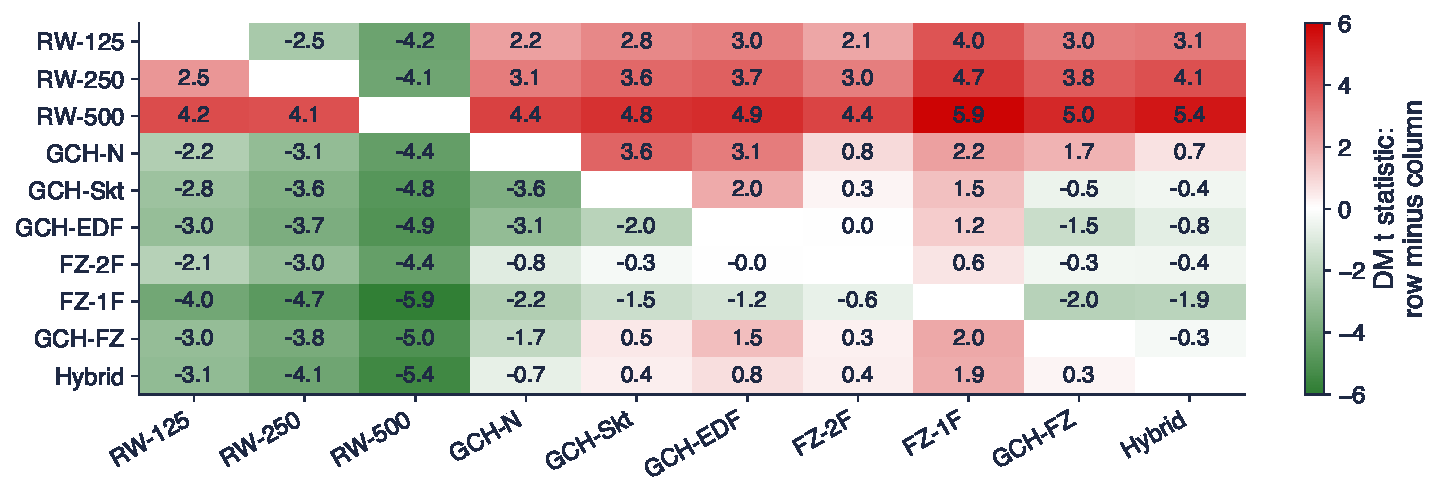
\includegraphics[width=0.97\textwidth,height=0.56\textheight,keepaspectratio]{ats_ch9_dm.pdf}
\end{center}
\vspace{-0.25cm}
\begin{itemize}
    \item S\&P 500, 2000--2016, $\alpha$ = 5\%: DM statistic of row minus column, Newey--West variance; red: the row model is worse (PZC, Table 9)
\end{itemize}
\quantlet{ATS\_ch9\_pzc}{\qlurl{ATS_ch9_pzc}}
\end{frame}

\begin{frame}{Interpreting the DM matrix}
\itemsize{\small}
\begin{itemize}
    \item Column GAS-1F, ours against PZC: RW-125 4.02 (3.91), RW-500 5.87 (5.48), GARCH-N 2.22 (1.99), GARCH-EDF 1.19 (1.20)
    \item The worst models are easily separated; the best few are not (GARCH-Skt, GARCH-EDF, FZ-2F against GAS-1F below 1.96)
    \item One difference: GARCH-FZ against GAS-1F, 2.02 here and 1.27 in the paper; the scale normalisation of GARCH-FZ makes its estimates fragile
    \item Ninety pairwise tests need a multiple-testing answer: the MCS (Section 6)
\end{itemize}
\end{frame}

\begin{frame}{Joint (VaR, ES) regression}
\itemsize{\small}
\begin{itemize}
    \item \refDB: both functionals are linear in the covariates
    \[ q_\alpha(Y_t \mid x_t) = x_t'\beta, \qquad -\mathrm{ES}_\alpha(Y_t \mid x_t) = x_t'\gamma \]
    \begin{itemize}
        \item $x_t$: covariates known at $t-1$; $\beta$, $\gamma$: the effects on the quantile and on the tail mean; estimated jointly by minimising a Fissler--Ziegel loss
        \item M-estimator: consistent and asymptotically normal for any member of the class; the choice of $(G_1, G_2)$ affects only efficiency
    \end{itemize}
    \item Uses
    \begin{itemize}
        \item which variables move the tail and by how much: the ES analogue of quantile regression
        \item ES backtests: regress realised returns on the ES forecast and test intercept 0, slope 1 \refBD\ (\atschlink{https://danpele.github.io/MFM/EN/Courses/chapter8_backtesting_risk.pdf}{MFM, Chapter 8})
    \end{itemize}
    \item Application: S\&P 500 returns 2000--2026 on the VIX of the previous close, $\alpha$ = 2.5\%, FZ0 loss, moving-block bootstrap standard errors (blocks of 20 days)
\end{itemize}
\end{frame}

\begin{frame}{The tail of the S\&P 500 against the VIX}
\itemsize{\footnotesize}
\begin{center}
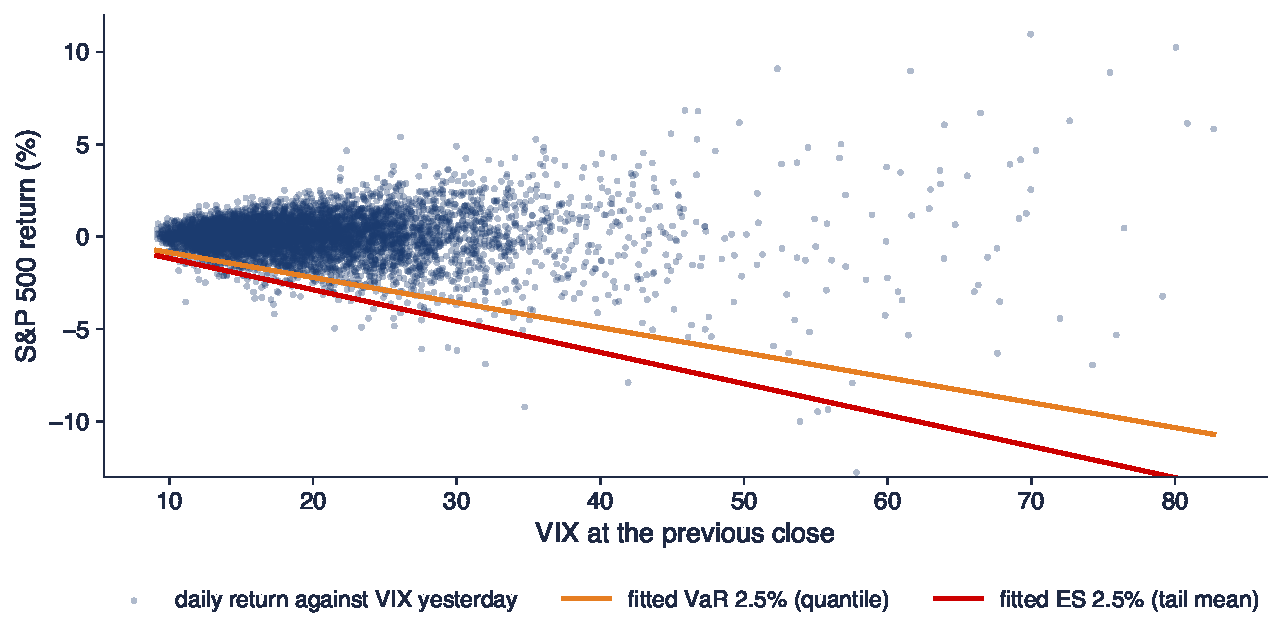
\includegraphics[width=0.97\textwidth,height=0.5\textheight,keepaspectratio]{ats_ch9_esreg.pdf}
\end{center}
\vspace{-0.25cm}
\begin{itemize}
    \item Daily returns against the VIX of the previous close, $T = 6\,714$; lines: fitted 2.5\% quantile and tail mean of the joint regression
\end{itemize}
\quantlet{ATS\_ch9\_esreg}{\qlurl{ATS_ch9_esreg}}
\end{frame}

\begin{frame}{Interpreting the joint regression}
\itemsize{\small}
\begin{itemize}
    \item Quantile: $0.499 \ensuremath{-}0.135\,\mathrm{VIX}$ (s.e.\ 0.150; 0.009); tail mean: $0.524 \ensuremath{-}0.170\,\mathrm{VIX}$ (s.e.\ 0.245; 0.015)
    \item One VIX point lowers the 2.5\% quantile by 0.14 and the tail mean by 0.17 percentage points: the tail fans out 1.25 times faster in ES
    \item The quantile part is close to quantile regression ($0.560$, $\ensuremath{-}0.139$); in-sample hit rate 2.50\%; the PZC tests do not reject ($p$ = 0.978; 0.744)
    \item The VIX is a market forecast of volatility: the regression says that the option market prices the left tail almost linearly
\end{itemize}
\end{frame}

\begin{frame}{Recap: Semiparametric (VaR, ES) models}
\itemsize{\small}
\begin{itemize}
    \item FZ0 minimisation estimates the tail pair without a distribution
    \item GAS forcing variables are identification functions: the model corrects itself only when the tail speaks
    \item The PZC ranking replicates; their goodness-of-fit results do not; joint regression links the tail to covariates
\end{itemize}
\end{frame}


%=============================================================================
\section{Backtesting as a test of calibration}
%=============================================================================

\begin{frame}{Recap: counting hits}
\itemsize{\small}
\begin{itemize}
    \item Hits $I_t = \mathbf 1\{y_t < v_t\}$; a correct VaR makes $I_t$ i.i.d.\ Bernoulli($\alpha$) (\atschlink{https://danpele.github.io/MFM/EN/Courses/chapter8_backtesting_risk.pdf}{MFM, Chapter 8})
    \begin{itemize}
        \item \refKup: unconditional coverage, likelihood-ratio statistic LR $\sim \chi^2_1$ (is the hit rate $\alpha$?)
        \item \refChr: independence of consecutive hits, and conditional coverage (both together), $\chi^2_2$
        \item Basel traffic light \refBCBS: green up to 4 hits of VaR 1\% in 250 days, yellow 5--9, red from 10
    \end{itemize}
    \item What counting misses
    \begin{itemize}
        \item hits that depend on information other than the last hit (DQ)
        \item the size of tail losses (ES backtests); the spacing of hits (duration tests)
        \item the effect of estimated parameters on the null distribution
    \end{itemize}
\end{itemize}
\end{frame}

\begin{frame}{Conditional calibration}
\itemsize{\small}
\begin{itemize}
    \item A forecast $x_t$ of $\mathrm T$ is \textbf{conditionally calibrated} if its identification function $V$ has conditional mean zero \refNZ
    \[ \E[V(x_t, Y_t) \mid \mathcal F_{t-1}] = 0 \ \Rightarrow\ \E[h_{t-1}V(x_t, Y_t)] = 0 \]
    \begin{itemize}
        \item $h_{t-1}$: any instrument known at $t-1$ (constant, lagged hits, the forecast itself); a moment test (Wald, $\chi^2$)
    \end{itemize}
    \item PZC, eq.~(40)--(41): standardised generalised residuals
    \[ \lambda^s_{v,t} = \mathbf 1\{y_t \le v_t\} - \alpha, \qquad \lambda^s_{e,t} = \frac{\mathbf 1\{y_t \le v_t\}\,y_t}{\alpha e_t} - 1 \]
    \begin{itemize}
        \item regress each on (1, its own first lag, $v_t$ or $e_t$) and test that all three coefficients are zero; we use a White (HC0) covariance
        \item DQ is the special case for VaR; the ES regression tests ES only jointly with VaR, as elicitability predicts
    \end{itemize}
    \item Power comes from the instruments: lagged hits detect clustering, the forecast level detects scale errors
\end{itemize}
\end{frame}

\begin{frame}{Duration-based backtests}
\itemsize{\small}
\begin{itemize}
    \item \refCP: under a correct VaR the durations $d_i$ (days between consecutive hits) are geometric, memoryless, with mean $1/\alpha$
    \begin{itemize}
        \item alternative: Weibull hazard $\lambda(d) = a^b b\,d^{b-1}$, the probability of a hit after $d$ quiet days; $a > 0$: scale, $b > 0$: shape
        \item $b = 1$: constant hazard (no memory, as under $H_0$); $b < 1$: decreasing hazard, i.e.\ hits cluster
    \end{itemize}
    \item Likelihood with censoring: the first and last spells are incomplete and enter through the survival function $S(d) = e^{-(ad)^b}$
    \[ \mathrm{LR} = 2\big[\ln L(\hat a, \hat b) - \ln L(\tilde a, 1)\big] \to \chi^2_1 \]
    \begin{itemize}
        \item $(\hat a, \hat b)$: unrestricted estimates; $\tilde a$: estimate under $b = 1$; small-sample p-values by simulation are advisable
    \end{itemize}
    \item Durations see clustering at any distance, not only on consecutive days as Christoffersen's test does
\end{itemize}
\end{frame}

\begin{frame}{How far apart are the hits?}
\itemsize{\footnotesize}
\begin{center}
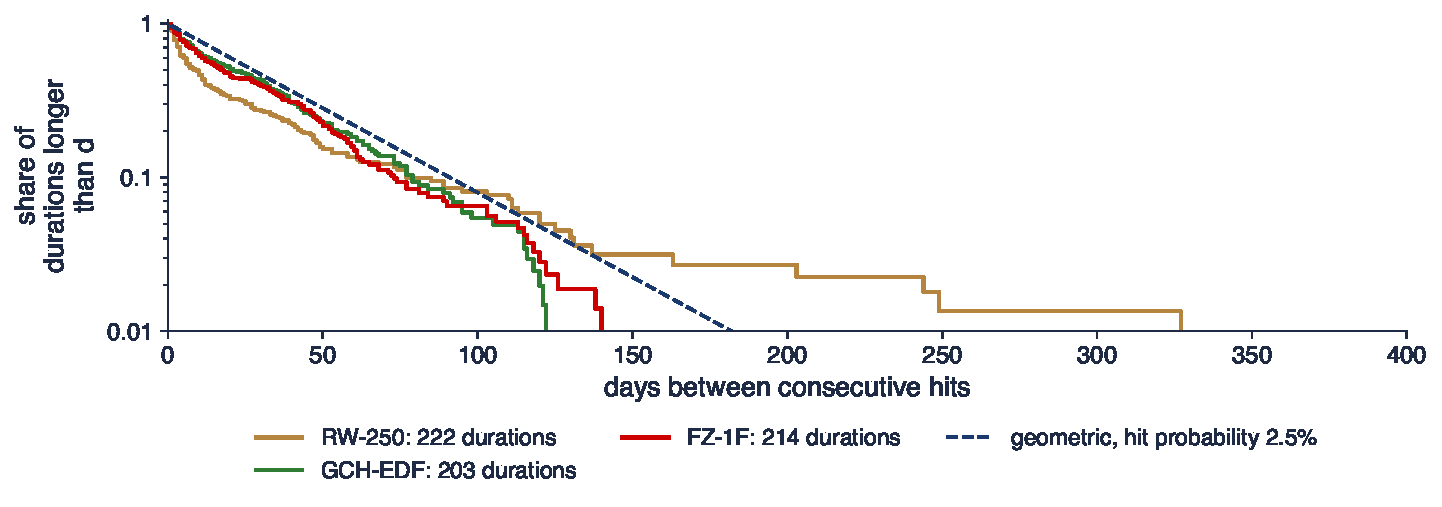
\includegraphics[width=0.97\textwidth,height=0.5\textheight,keepaspectratio]{ats_ch9_durations.pdf}
\end{center}
\vspace{-0.25cm}
\begin{itemize}
    \item S\&P 500, VaR 2.5\%, out of sample 2000--2026; empirical survival of the durations between hits (log scale) against the geometric law of a correct model
\end{itemize}
\quantlet{ATS\_ch9\_backtests}{\qlurl{ATS_ch9_backtests}}
\end{frame}

\begin{frame}{Interpreting the durations}
\itemsize{\small}
\begin{itemize}
    \item RW-250: 40\% of the durations are at most 5 days (geometric: 12\%); Weibull $b$ = 0.67, $p$ $<$0.001: strong clustering
    \item GARCH-EDF: $b$ = 0.92, $p$ = 0.107; GAS-1F: $b$ = 0.88, $p$ = 0.019: dynamic models remove most of the clustering
    \item The long tail of RW-250 (calm years without hits) is the other face of clustering: the window remembers old crises
    \item All models have too many hits overall (Section 5 table): parameters fixed in 1999 are too optimistic after 2000
\end{itemize}
\end{frame}

\begin{frame}{Backtesting ES: what each test needs}
\itemsize{\footnotesize}
\begin{center}
\scriptsize
\begin{tabular}{>{\raggedright\arraybackslash}p{3.2cm}>{\raggedright\arraybackslash}p{4.5cm}>{\raggedright\arraybackslash}p{3.8cm}}
\toprule
\textbf{Test} & \textbf{Statistic} & \textbf{Inputs} \\
\midrule
\refMF{} & mean of $(y_t - e_t)/\sigma_t$ on hit days, bootstrap & $v_t$, $e_t$, $\sigma_t$ \\
\refAS\ $Z_2$ & $1 - \frac{1}{T\alpha}\sum_t \frac{y_tI_t}{e_t}$ & $v_t$, $e_t$ and the forecast distribution (simulated $p$-value) \\
\refDE{} & cumulative violations $H_t = \frac{1}{\alpha}(\alpha - u_t)\mathbf 1\{u_t \le \alpha\}$ & the PIT $u_t = F_{t|t-1}(y_t)$ \\
\refKLM{} & multinomial test of several VaR levels & the PIT, or VaR at several levels \\
\refPZC, \refBD{} & regression on $(v_t, e_t)$ & $v_t$, $e_t$ \\
\bottomrule
\end{tabular}
\end{center}
\begin{itemize}
    \item $\sigma_t$: forecast volatility; $I_t$: hit indicator; $u_t = F_{t|t-1}(y_t)$: probability integral transform (PIT), uniform on $[0, 1]$ under a correct forecast distribution
    \item Only the regression tests use nothing beyond the pair (VaR, ES): the others are tests of a distribution, which ES alone does not supply
\end{itemize}
\end{frame}

\begin{frame}{Estimation risk in backtests}
\itemsize{\small}
\begin{itemize}
    \item Backtests assume the VaR is known; in practice $\hat v_t = v_t(\hat\theta_R)$, estimated on $R$ days and tested on the next $P$ days \refEO
    \[ \frac{1}{\sqrt P}\sum_t(\hat I_t - \alpha) = \frac{1}{\sqrt P}\sum_t(I_t - \alpha) + \underbrace{\sqrt{P/R}\cdot\E[f_t(v_t)\nabla v_t']\,\sqrt R(\hat\theta_R - \theta)}_{\text{estimation term}} \]
    \begin{itemize}
        \item $\hat I_t$, $I_t$: hits of the estimated and of the true VaR; $f_t(v_t)$: conditional density at the VaR; $\nabla v_t$: gradient of the VaR in $\theta$
    \end{itemize}
    \item The estimation term vanishes only if $P/R \to 0$; with a fixed window it grows with the test sample
    \begin{itemize}
        \item the Kupiec variance $\alpha(1 - \alpha)$ is then too small and the test over-rejects a correct model
        \item fixes: the corrected variance of Escanciano and Olmo, a subsampling or bootstrap of the whole estimate-and-test procedure
    \end{itemize}
    \item A Monte Carlo shows the size of the problem for the windows banks actually use
\end{itemize}
\end{frame}

\begin{frame}{Size of backtests with estimated parameters}
\itemsize{\footnotesize}
\begin{center}
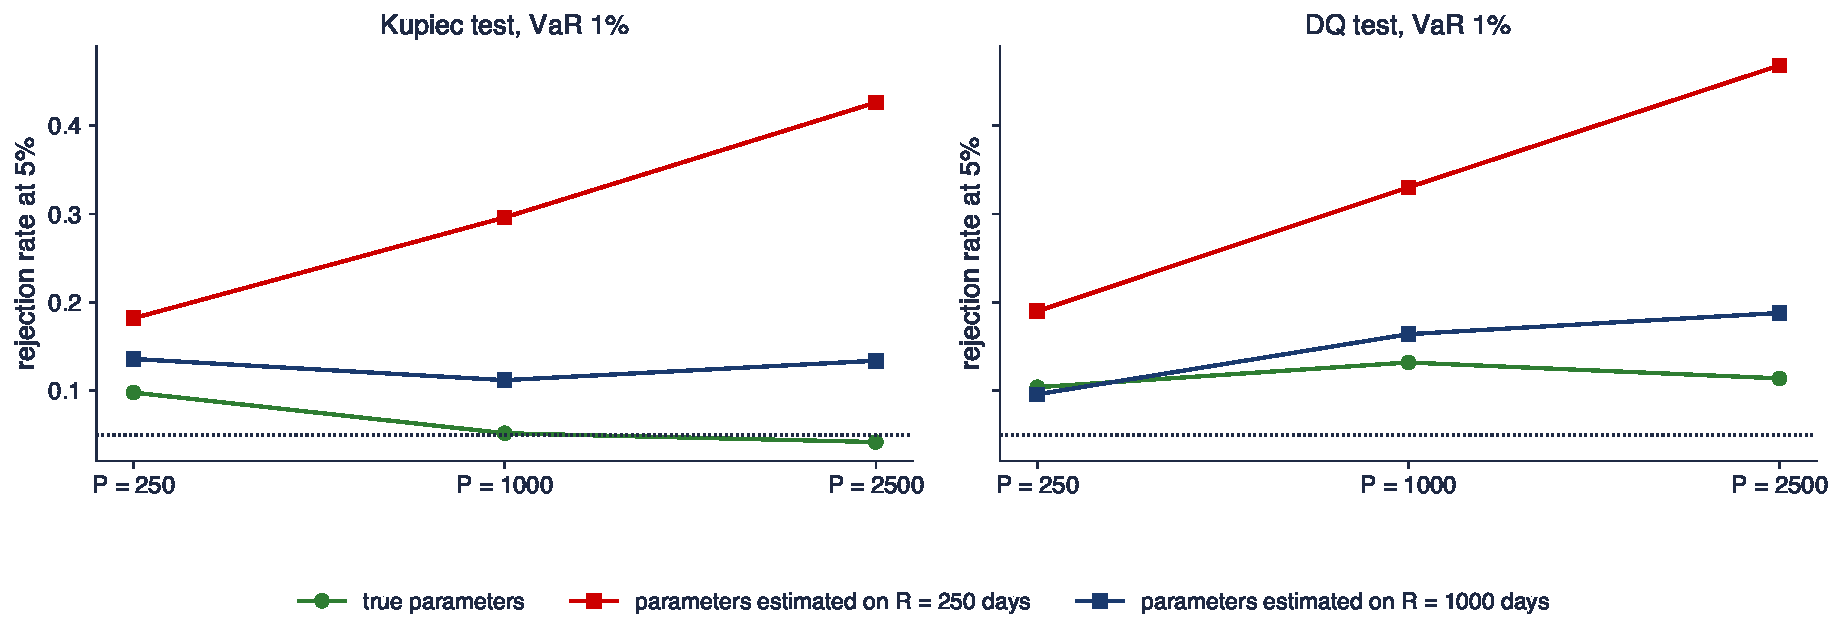
\includegraphics[width=0.97\textwidth,height=0.5\textheight,keepaspectratio]{ats_ch9_estrisk_mc.pdf}
\end{center}
\vspace{-0.25cm}
\begin{itemize}
    \item GARCH(1,1) data ($\omega$ = 0.02, $\alpha$ = 0.08, $\beta$ = 0.90, Normal), the correct model estimated by QML on $R$ days, VaR 1\% on the next $P$ days; 500 replications; nominal size 5\%
\end{itemize}
\quantlet{ATS\_ch9\_backtests}{\qlurl{ATS_ch9_backtests}}
\end{frame}

\begin{frame}{Interpreting the Monte Carlo}
\itemsize{\small}
\begin{itemize}
    \item Known parameters: Kupiec rejects 10\%, 5\% and 4\% for $P$ = 250, 1000, 2500: close to 5\% except with few hits
    \item Estimated on $R$ = 250: 18\%, 30\%, 43\%: a correct model is rejected more often the longer we test
    \item With $R$ = 1000 the distortion shrinks (13\% at $P$ = 2500); the hit rate across replications has s.d.\ 0.99 pp against 0.29 pp
    \item DQ is oversized even with known parameters (10\%): rare hits make the $\chi^2_6$ approximation poor
\end{itemize}
\end{frame}

\begin{frame}{Calibration tests across assets}
\itemsize{\footnotesize}
\begin{center}
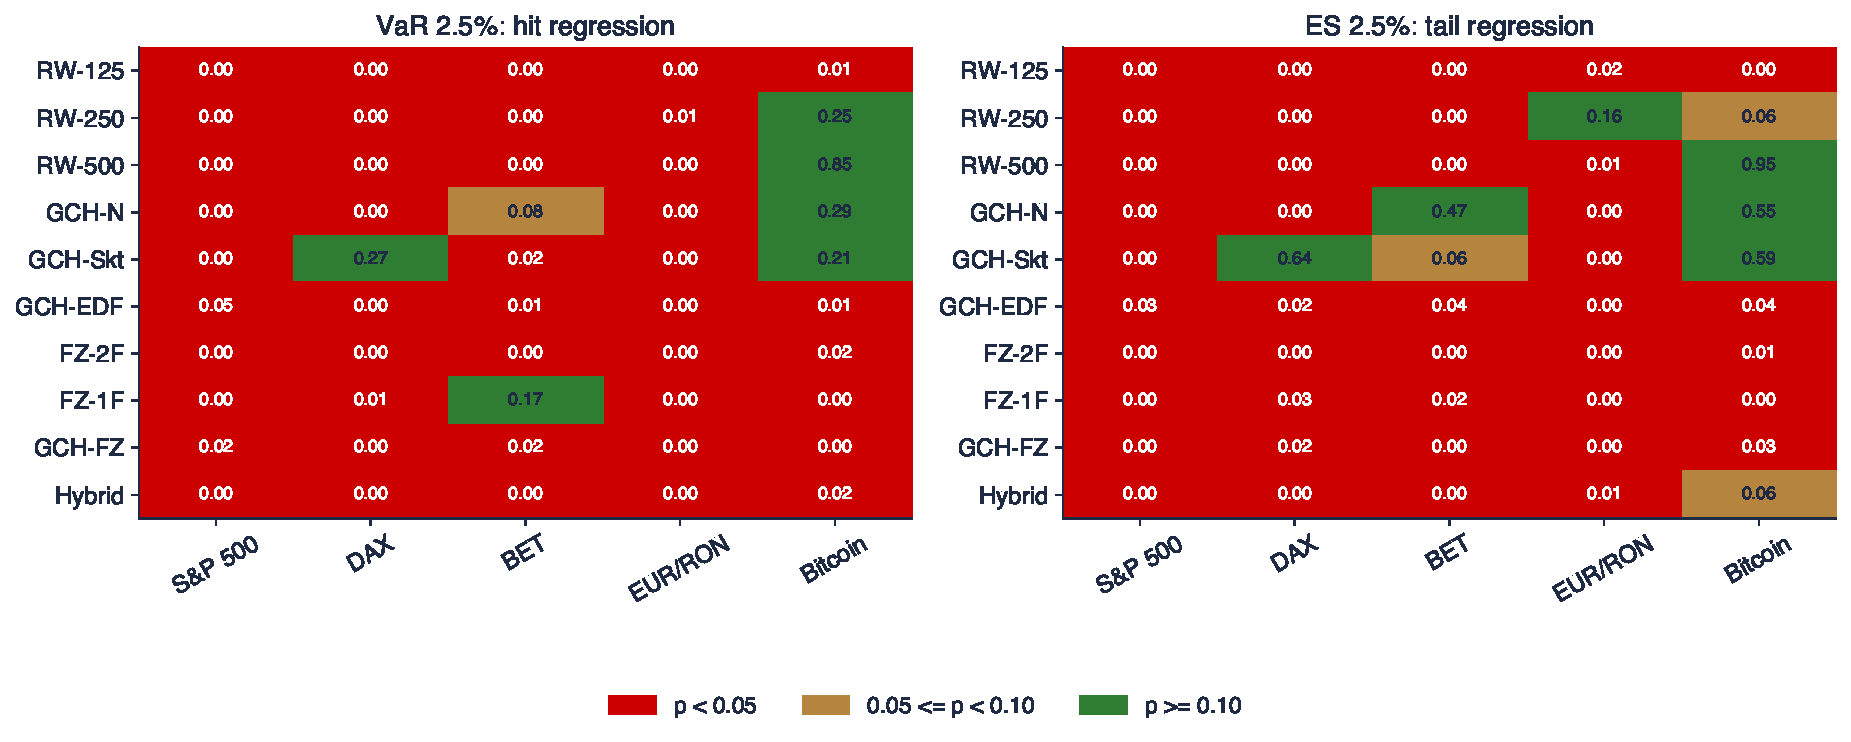
\includegraphics[width=0.97\textwidth,height=0.52\textheight,keepaspectratio]{ats_ch9_backtests.pdf}
\end{center}
\vspace{-0.25cm}
\begin{itemize}
    \item PZC goodness-of-fit regressions for VaR and ES 2.5\%, ten models, parameters estimated on the first ten years (five for Bitcoin) and kept fixed to 18 September 2026
\end{itemize}
\quantlet{ATS\_ch9\_backtests}{\qlurl{ATS_ch9_backtests}}
\end{frame}

\begin{frame}{Interpreting the calibration tests}
\itemsize{\footnotesize}
\begin{itemize}
    \item Only 4 of 50 asset--model pairs pass both regressions at 10\%: over 10--26 years with fixed parameters almost every model is miscalibrated somewhere
    \item S\&P 500 hit rates at 2.5\%: GAS-1F 3.2\%, GARCH-EDF 3.0\%, RW-250 3.3\%: the level drifts after the estimation decade
    \item EUR/RON: estimated on 2005--2015 (crisis and float), the GARCH models over-predict risk afterwards (GARCH-EDF 0.6\% hits): miscalibration in the safe direction is rejected too
    \item Bitcoin: short history and noisy tail, low power; the simple models pass (RW-500 2.5\%)
    \item A backtest answers ``is it calibrated?''; whether to prefer one failing model to another is a comparison question
\end{itemize}
\end{frame}

\begin{frame}{Recap: Backtesting}
\itemsize{\small}
\begin{itemize}
    \item Backtests are moment tests of the identification function with chosen instruments
    \item Durations catch clustering at any distance; ES tests need more than ES, except the regression tests
    \item Estimated parameters inflate the size; long, fixed-parameter evaluations reject almost everything
\end{itemize}
\end{frame}


%=============================================================================
\section{Comparing risk forecasts}
%=============================================================================

\begin{frame}{From backtests to comparative backtests}
\itemsize{\small}
\begin{itemize}
    \item \refNZ: a traditional backtest tests $H_0$: ``the bank's model is calibrated''; a comparative backtest tests the bank's model against a standard one with a consistent score
    \begin{itemize}
        \item $H_0^-$: internal at least as good as standard; $H_0^+$: at most as good; green if $H_0^+$ is rejected, red if $H_0^-$ is rejected, yellow otherwise
    \end{itemize}
    \item Information sets matter \refHE: a calibrated forecast based on more information has a lower expected consistent score
    \begin{itemize}
        \item so a ranking by FZ0 rewards both calibration and information, which a backtest cannot do
    \end{itemize}
    \item Tools from \atschlink{https://danpele.github.io/Advanced-Time-Series/EN/Courses/chapter1_forecast_evaluation.pdf}{Chapter 1}: DM with HAC variance \refDM, Giacomini--White for estimated forecasting methods \refGW, the MCS \refHLN
\end{itemize}
\end{frame}

\begin{frame}{Design of the comparison}
\itemsize{\small}
\begin{itemize}
    \item Ten PZC models, $\alpha$ = 2.5\%, FZ0 losses out of sample: S\&P 500 and DAX from 2000, BET from 2010, EUR/RON from July 2015, Bitcoin from 2020
    \item 90\% MCS with the $T_{\max}$ statistic, moving-block bootstrap (blocks of 10 days over the whole period, 5 days in a stress period), 1000 replications
    \item Stress periods fixed before looking at the losses
    \begin{itemize}
        \item 2008: September 2008 -- March 2009; 2020: 19 February -- 30 June 2020; 2022: the calendar year; 2025: March -- June 2025
        \item S\&P 500 in 2020: 93 days, of which 9 GAS-1F hits; in 2025: 83 days, 5 hits
    \end{itemize}
    \item A stress window holds a few tail days: expect wide MCS sets and unstable winners
\end{itemize}
\end{frame}

\begin{frame}{Losses in stress periods}
\itemsize{\footnotesize}
\begin{center}
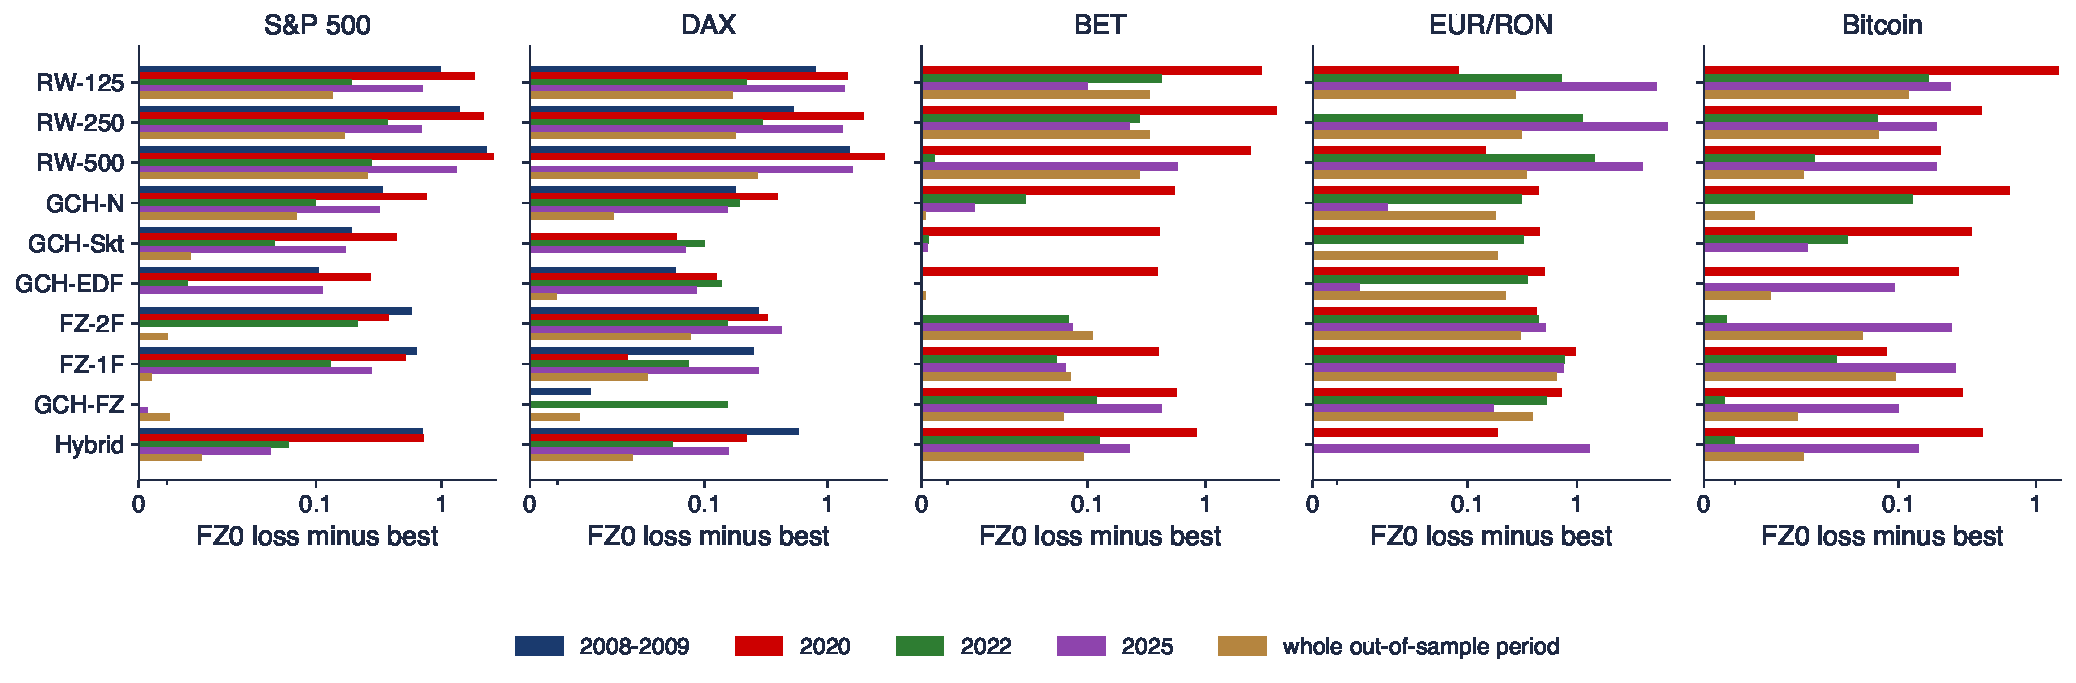
\includegraphics[width=0.97\textwidth,height=0.52\textheight,keepaspectratio]{ats_ch9_stress.pdf}
\end{center}
\vspace{-0.25cm}
\begin{itemize}
    \item Average FZ0 loss of each model minus that of the best model in the same period (symmetric log scale); bars missing when the period is not out of sample
\end{itemize}
\quantlet{ATS\_ch9\_comparison}{\qlurl{ATS_ch9_comparison}}
\end{frame}

\begin{frame}{Interpreting the stress-period losses}
\itemsize{\footnotesize}
\begin{itemize}
    \item Winners over the whole period: S\&P 500 GCH-EDF, DAX GCH-Skt, BET GCH-Skt, EUR/RON Hybrid, Bitcoin GCH-Skt
    \item In 2020 the winner changes: S\&P 500 GCH-FZ, BET FZ-2F, Bitcoin FZ-2F; rolling windows lose most in every crash
    \item Crashes separate models by an order of magnitude more than calm years: an average over the whole period is dominated by a few weeks
    \item No model wins every crisis; the semiparametric models are competitive but not dominant out of sample after 2016
\end{itemize}
\end{frame}

\begin{frame}{Model confidence sets}
\itemsize{\footnotesize}
\begin{center}
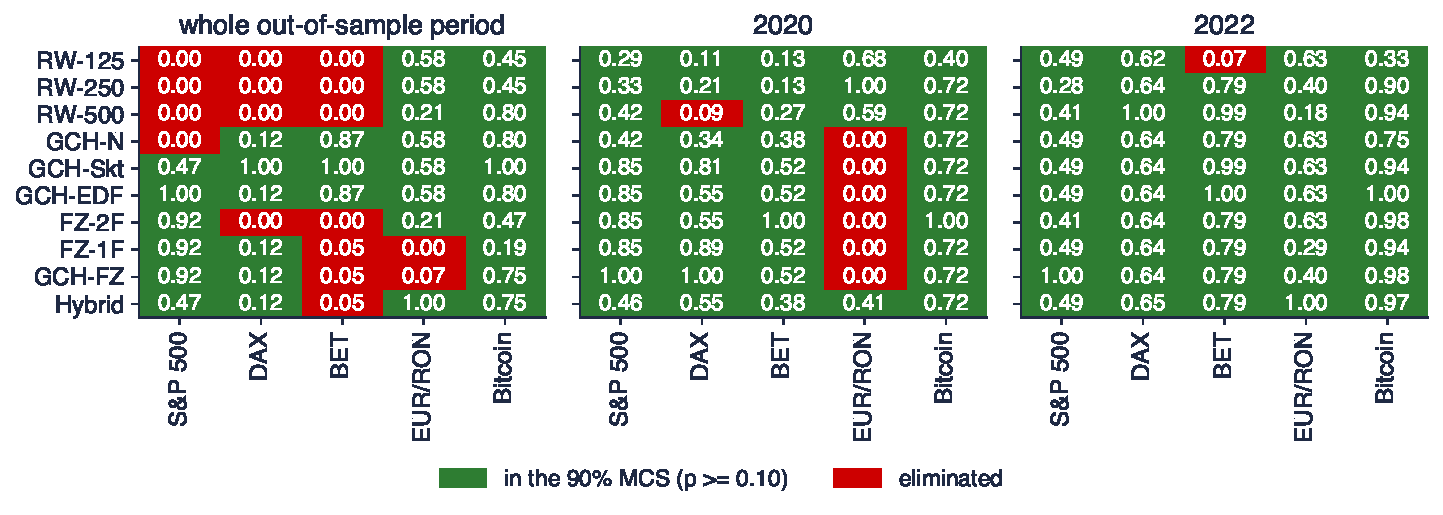
\includegraphics[width=0.97\textwidth,height=0.52\textheight,keepaspectratio]{ats_ch9_mcs.pdf}
\end{center}
\vspace{-0.25cm}
\begin{itemize}
    \item MCS $p$-values (FZ0 loss, $\alpha$ = 2.5\%); green: in the 90\% MCS
\end{itemize}
\quantlet{ATS\_ch9\_comparison}{\qlurl{ATS_ch9_comparison}}
\end{frame}

\begin{frame}{Interpreting the MCS}
\itemsize{\small}
\begin{itemize}
    \item Whole period, MCS sizes: S\&P 500 6, DAX 6, BET 3, EUR/RON 8, Bitcoin 10 of 10
    \item Rolling windows are eliminated on the long equity samples; in 2020 and 2022 almost everything survives (2020: 10 on the S\&P 500; 2022: 10)
    \item EUR/RON in 2020 is the exception: only 4 models survive, the rolling windows and the Hybrid
    \item A large MCS is a result, not a failure: the crisis windows are too short to separate tail forecasts
\end{itemize}
\end{frame}

\begin{frame}{Recap: Comparison}
\itemsize{\small}
\begin{itemize}
    \item Comparative backtests put the burden of proof on the model, and reward information
    \item Rankings change in crises; whole-period averages hide this
    \item Report the MCS, not the winner
\end{itemize}
\end{frame}


%=============================================================================
\section{The horizon: multi-period risk}
%=============================================================================

\begin{frame}{Why the square-root-of-time rule fails (1/2)}
\itemsize{\small}
\begin{itemize}
    \item The rule scales the one-day VaR to $h$ days
    \[ \mathrm{VaR}^{(h)} = \sqrt h\,\mathrm{VaR}^{(1)} \]
    \begin{itemize}
        \item $\mathrm{VaR}^{(h)}$: VaR of the $h$-day return $\sum_{k=1}^h y_{t+k}$; exact for i.i.d.\ returns from the Normal distribution with zero mean
        \item for i.i.d.\ stable laws with index $\gamma \in (0, 2]$ the factor is $h^{1/\gamma}$ ($\gamma = 2$: the Normal case)
    \end{itemize}
    \item Fat tails that are not stable: the $h$-day sum is closer to Normal than the daily return
    \begin{itemize}
        \item so $\sqrt h$ overstates the quantile at long horizons \refDZ
    \end{itemize}
    \item Leverage (GJR) makes multi-day losses more skewed than daily ones: the left tail of the sum is thicker than the scaled daily tail
\end{itemize}
\end{frame}

\begin{frame}{Why the square-root-of-time rule fails (2/2)}
\itemsize{\small}
\begin{itemize}
    \item Volatility clustering: for GARCH(1,1) the variance of the $h$-day return depends on today's volatility
    \[ \mathrm{Var}_t\Big(\sum_{k=1}^h y_{t+k}\Big) = \sum_{k=0}^{h-1}\big[\bar\sigma^2 + (\alpha + \beta)^k(\sigma_{t+1}^2 - \bar\sigma^2)\big] \]
    \begin{itemize}
        \item $\bar\sigma^2 = \omega/(1 - \alpha - \beta)$: unconditional variance; $\sigma^2_{t+1}$: tomorrow's forecast variance; $\alpha + \beta$: persistence
        \item in calm times ($\sigma^2_{t+1} < \bar\sigma^2$) $\sqrt h$ understates risk, in crises it overstates it: mean reversion of volatility
    \end{itemize}
    \item Remedies: simulate the $h$-day distribution (FHS), or forecast the $h$-day quantile directly (quantile regression on $h$-day returns)
\end{itemize}
\end{frame}

\begin{frame}{Multi-day forecasts and their backtests}
\itemsize{\small}
\begin{itemize}
    \item FHS: GJR-GARCH(1,1) by QML \refBoll, \refGJR
    \begin{itemize}
        \item rolling 2000-day window, re-estimated every 250 days
        \item 2000 paths of 10 days with bootstrapped standardised residuals
    \end{itemize}
    \item Backtesting 10-day VaR
    \begin{itemize}
        \item daily 10-day forecasts overlap: hits are MA(9) even under $H_0$; counting them as independent inflates the size (\atschlink{https://danpele.github.io/Advanced-Time-Series/EN/Courses/chapter0_refresher_inference.pdf}{Chapter 0}, overlapping observations)
        \item options: non-overlapping windows (every 10th day, few hits), or HAC variance on overlapping hits
    \end{itemize}
    \item Basel uses 10-day horizons and liquidity-adjusted horizons for ES (MAR33): the horizon problem is regulatory, not academic
\end{itemize}
\end{frame}

\begin{frame}{10-day VaR 1\% against the square-root-of-time rule}
\itemsize{\footnotesize}
\begin{center}
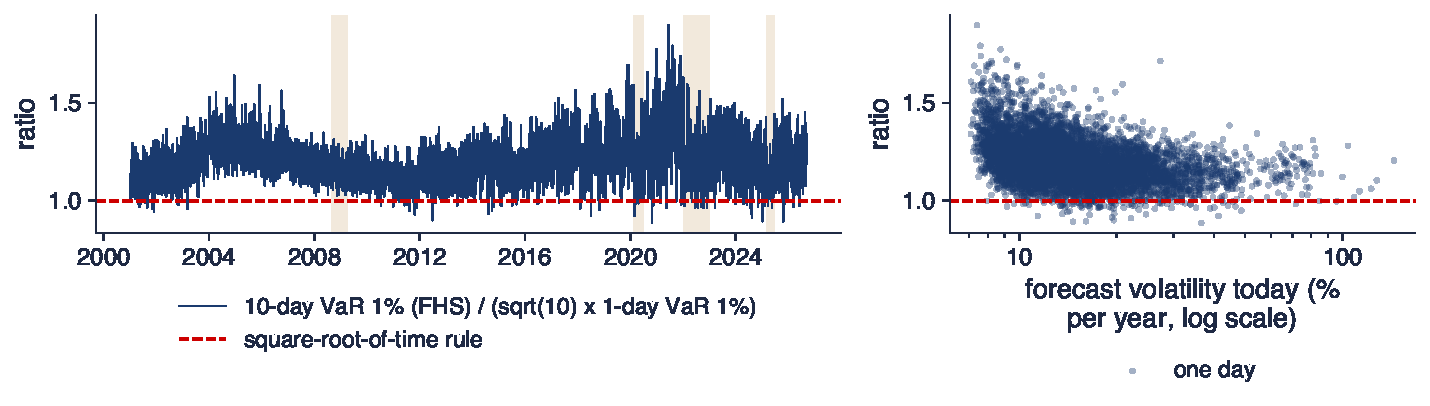
\includegraphics[width=0.97\textwidth,height=0.5\textheight,keepaspectratio]{ats_ch9_sqrt.pdf}
\end{center}
\vspace{-0.25cm}
\begin{itemize}
    \item S\&P 500, 2001--2026: ratio of the 10-day VaR 1\% by FHS to $\sqrt{10}$ times the 1-day VaR 1\% of the same model; right: the ratio against today's forecast volatility
\end{itemize}
\quantlet{ATS\_ch9\_horizon}{\qlurl{ATS_ch9_horizon}}
\end{frame}

\begin{frame}{Interpreting the horizon ratio}
\itemsize{\small}
\begin{itemize}
    \item Median ratio 1.19, range 0.89 to 1.90: $\sqrt{10}$ scaling usually understates the 10-day VaR 1\% of the S\&P 500
    \item Low-volatility days: median 1.26; high-volatility days: 1.14: mean reversion pushes the ratio towards 1 in crises
    \item Non-overlapping backtest (646 windows, 6.5 expected hits): FHS 6, $\sqrt{10}$ rule 7; Kupiec $p$ 0.85 and 0.83
    \item So few hits cannot separate the two: horizon errors of this size are invisible to a non-overlapping backtest
\end{itemize}
\end{frame}

\begin{frame}{Recap: The horizon}
\itemsize{\small}
\begin{itemize}
    \item The square-root rule needs i.i.d.\ Normal returns; clustering, leverage and fat tails break it in opposite directions
    \item Simulate the horizon or model it directly; backtest with non-overlapping windows or HAC variances
    \item Multi-day tests have very little power
\end{itemize}
\end{frame}


%=============================================================================
\section{Model risk and estimation risk}
%=============================================================================

\begin{frame}{Model risk of risk models}
\itemsize{\small}
\begin{itemize}
    \item \refDJVZ: the \textbf{risk ratio} across standard models measures the disagreement a regulator should expect
    \[ \mathrm{RR}_t = \frac{\max_m\mathrm{VaR}_{m,t}}{\min_m\mathrm{VaR}_{m,t}} \ge 1 \]
    \begin{itemize}
        \item $\mathrm{VaR}_{m,t}$: the forecast of model $m$ for day $t$; $\mathrm{RR}_t = 1$: all models agree; 2: the most prudent model asks for twice the capital of the least prudent
        \item they find the ratio largest exactly in crises, when risk numbers matter most
    \end{itemize}
    \item \refBDKM: \textbf{risk models-at-risk}: quantify the model risk of a VaR forecast and adjust the forecast for estimation and specification errors
    \item \refKR: ES carries more model risk than VaR at comparable levels: it extrapolates further into the tail
    \item Our six models, rolling 1000-day windows: historical simulation, Normal with window volatility, EWMA ($\lambda$ = 0.94), GARCH-N, GARCH-t, filtered HS
\end{itemize}
\end{frame}

\begin{frame}{How much do standard models disagree?}
\itemsize{\footnotesize}
\begin{center}
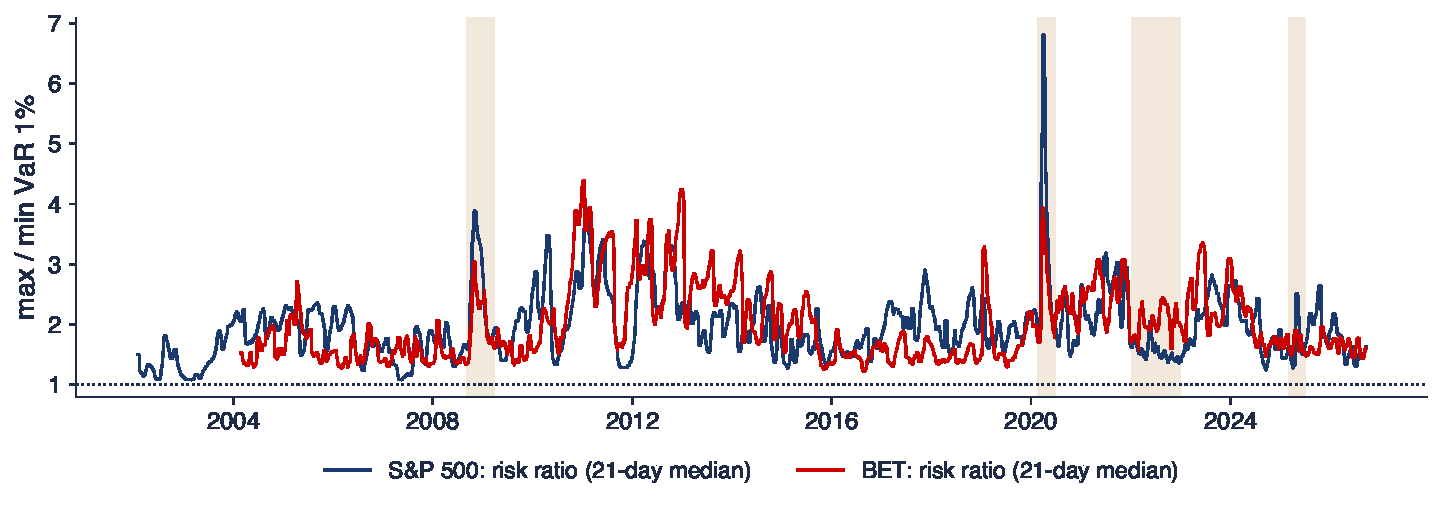
\includegraphics[width=0.97\textwidth,height=0.5\textheight,keepaspectratio]{ats_ch9_riskratio.pdf}
\end{center}
\vspace{-0.25cm}
\begin{itemize}
    \item Risk ratio of six VaR 1\% forecasts, 21-day rolling median, S\&P 500 and BET, 2002--2026 (BET from 2004); shaded: stress periods
\end{itemize}
\quantlet{ATS\_ch9\_modelrisk}{\qlurl{ATS_ch9_modelrisk}}
\end{frame}

\begin{frame}{Interpreting the risk ratio}
\itemsize{\footnotesize}
\begin{itemize}
    \item Median risk ratio 1.9 (S\&P 500) and 1.8 (BET); 90th percentile 2.7 and 3.0; maximum 10.5 on 17 March 2020
    \item Spring 2020: median 2.9 (S\&P 500), 2.5 (BET): the slow historical simulation and the fast EWMA diverge most after a jump
    \item HS is the most conservative model on 73\% of S\&P 500 days, EWMA the least on 53\%
    \item Hit rates for VaR 1\% (S\&P 500): HS 1.4\%, GARCH-N 2.2\%, GARCH-t 1.4\%, FHS 1.3\%: the disagreement is not noise, the Normal models are wrong
\end{itemize}
\end{frame}

\begin{frame}{Estimation risk in tail forecasts}
\itemsize{\small}
\begin{itemize}
    \item \refGS: for GARCH VaR and ES, $\sqrt T(\widehat{\mathrm{ES}}_t - \mathrm{ES}_t)$ is asymptotically normal; the variance has a volatility part and a tail-shape part
    \item Bootstrap \refCG: re-estimate the model on simulated paths and recompute the forecast \textbf{conditional on the observed history}
    \begin{itemize}
        \item algorithm: fit GARCH-t on 2000 days; simulate 150 paths of 2000 days from the fit; re-estimate on each; filter the observed returns with each $\hat\theta^*$; ES$^*$ for tomorrow
        \item 90\% interval: the 5\% and 95\% quantiles of ES$^*$
    \end{itemize}
    \item The interval measures parameter uncertainty only: it is conditional on the model being right, so it is a lower bound on total uncertainty
\end{itemize}
\end{frame}

\begin{frame}{An ES forecast with its estimation error}
\itemsize{\footnotesize}
\begin{center}
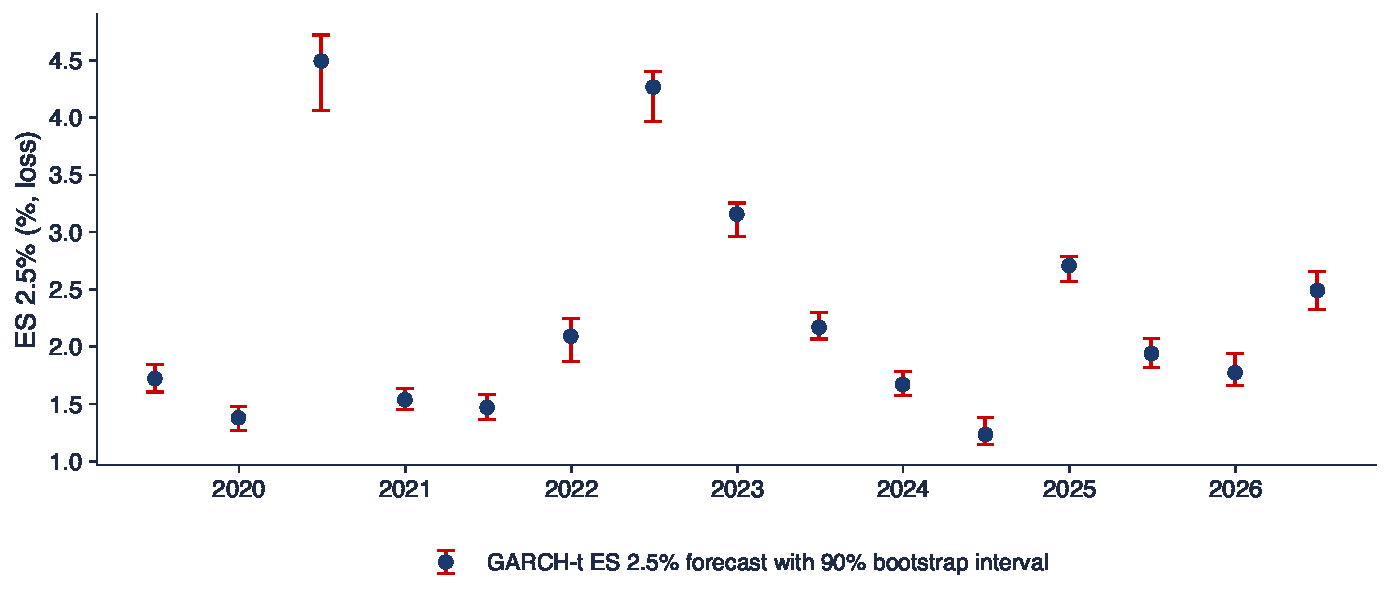
\includegraphics[width=0.97\textwidth,height=0.5\textheight,keepaspectratio]{ats_ch9_es_ci.pdf}
\end{center}
\vspace{-0.25cm}
\begin{itemize}
    \item S\&P 500, GARCH-t ES 2.5\% for the next day at half-year ends 2019--2026, with 90\% parametric bootstrap intervals (150 re-estimations each)
\end{itemize}
\quantlet{ATS\_ch9\_modelrisk}{\qlurl{ATS_ch9_modelrisk}}
\end{frame}

\begin{frame}{Interpreting the estimation error}
\itemsize{\small}
\begin{itemize}
    \item Interval width relative to the forecast: median 13\%, from 8\% to 19\%
    \item June 2020: ES 4.49\% with interval [4.06; 4.72]: two thousand days of data still leave a band of several tenths of a percent
    \item Estimation risk is small next to model risk (risk ratios near 2): the choice of model matters more than its precision
    \item Capital rules that multiply a point forecast ignore both: reporting the interval is the honest minimum
\end{itemize}
\end{frame}

\begin{frame}{Recap: Model and estimation risk}
\itemsize{\small}
\begin{itemize}
    \item Standard models disagree by a factor of about two, more in crises
    \item Bootstrap intervals for ES are narrow next to that disagreement
    \item Report both: the forecast, its interval and the spread across models
\end{itemize}
\end{frame}


%=============================================================================
\section{Extremes under dependence and conformal calibration}
%=============================================================================

\begin{frame}{Extremes of dependent series}
\itemsize{\small}
\begin{itemize}
    \item For a stationary series, dependence changes the law of the maximum only through one number, the \textbf{extremal index} $\theta$ \refEKM
    \[ \Pr\Big(\max_{t \le n} X_t \le u_n\Big) \approx F(u_n)^{n\theta}, \qquad \theta \in (0, 1] \]
    \begin{itemize}
        \item $X_t$: the daily loss; $F$: its marginal distribution; $u_n$: a high threshold that grows with the sample size $n$
        \item $1/\theta$ = mean cluster size of exceedances; $\theta = 1$: no clustering of extremes
    \end{itemize}
    \item Intervals estimator \refFS, from the gaps $T_i$ between the $N$ exceedances (when $\max T_i > 2$)
    \[ \hat\theta = \min\Big(1, \frac{2\big(\sum_i(T_i - 1)\big)^2}{(N - 1)\sum_i(T_i - 1)(T_i - 2)}\Big) \]
    \item \refMF: fit GARCH, apply EVT to the standardised residuals; it works if filtering removes the clustering ($\theta$ near 1 after filtering)
\end{itemize}
\end{frame}

\begin{frame}{Extremal index before and after filtering}
\itemsize{\footnotesize}
\begin{center}
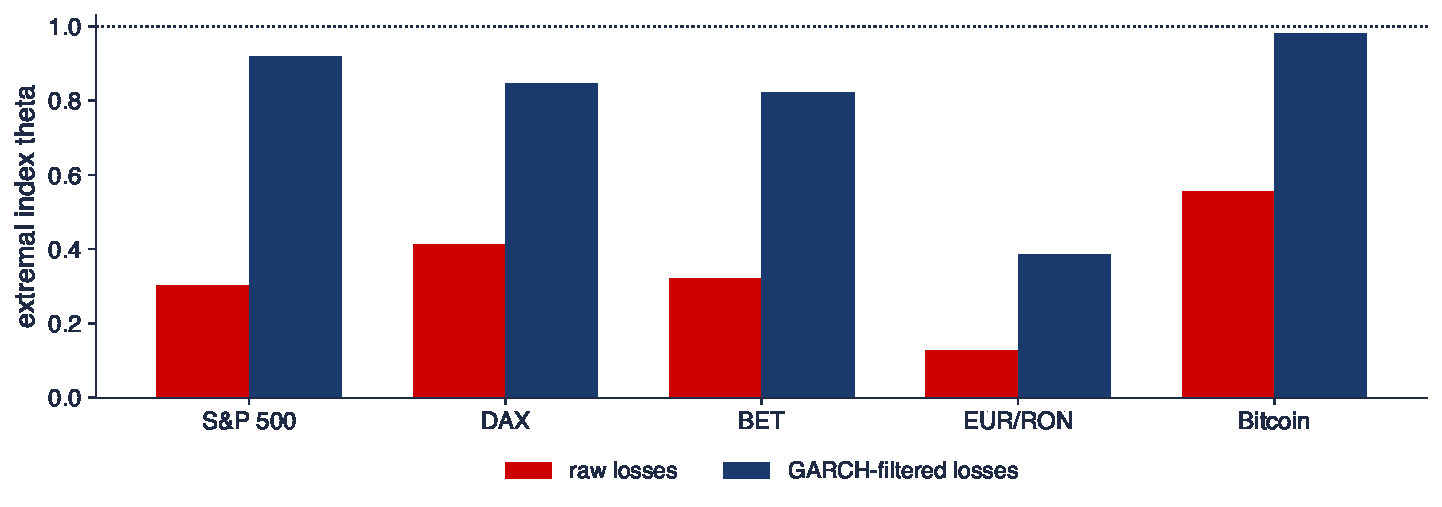
\includegraphics[width=0.97\textwidth,height=0.48\textheight,keepaspectratio]{ats_ch9_extremal.pdf}
\end{center}
\vspace{-0.25cm}
\begin{itemize}
    \item Exceedances of daily losses over their 95\% quantile, whole samples; raw losses and GARCH-standardised losses (in-sample ARMA-GARCH parameters)
\end{itemize}
\quantlet{ATS\_ch9\_extremes}{\qlurl{ATS_ch9_extremes}}
\end{frame}

\begin{frame}{Interpreting the extremal index}
\itemsize{\small}
\begin{itemize}
    \item Raw losses: $\hat\theta$ = 0.30 (S\&P 500), 0.32 (BET), 0.13 (EUR/RON): extremes come in clusters of two to eight days
    \item After filtering: 0.92, 0.85, 0.98 for the S\&P 500, DAX and Bitcoin: GARCH removes most of the clustering, as McNeil and Frey assume
    \item EUR/RON stays clustered (0.39) and BET partly (0.82): a managed exchange rate and a thin market have dependence that GARCH does not capture
    \item With fixed in-sample parameters the filter is imperfect after the estimation period: part of the remaining clustering is drift
\end{itemize}
\end{frame}

\begin{frame}{Conformal calibration of VaR}
\itemsize{\small}
\begin{itemize}
    \item Split conformal quantiles guarantee coverage under exchangeability (\atschlink{https://danpele.github.io/Advanced-Time-Series/EN/Courses/chapter13_foundation_models_conformal.pdf}{Chapter 13}); returns are not exchangeable, so the guarantee fails
    \item \textbf{Adaptive conformal inference} (ACI) \refGC: forecast at a working level $\alpha_t$ and correct it after each day
    \[ \alpha_{t+1} = \alpha_t + \gamma(\alpha - \mathrm{err}_t), \qquad \mathrm{err}_t = \mathbf 1\{y_t < q_t(\alpha_t)\} \]
    \begin{itemize}
        \item $q_t(\alpha_t)$: the model's quantile at level $\alpha_t$; $\gamma > 0$: step size; after a hit $\alpha_{t+1}$ falls (VaR rises), after a quiet day it rises slightly
        \item deterministic guarantee: $\big|T^{-1}\sum_t\mathrm{err}_t - \alpha\big| \le \dfrac{\max(\alpha_1, 1 - \alpha_1) + \gamma}{\gamma T}$ for \textbf{any} sequence of returns ($\alpha_1$: the starting level)
        \item long-run frequency only: no conditional calibration, no statement about ES
    \end{itemize}
    \item Further reading: conformal recalibration of extreme tail quantiles under dependence \refCO
\end{itemize}
\end{frame}

\begin{frame}{Adaptive conformal correction of VaR 1\%}
\itemsize{\footnotesize}
\begin{center}
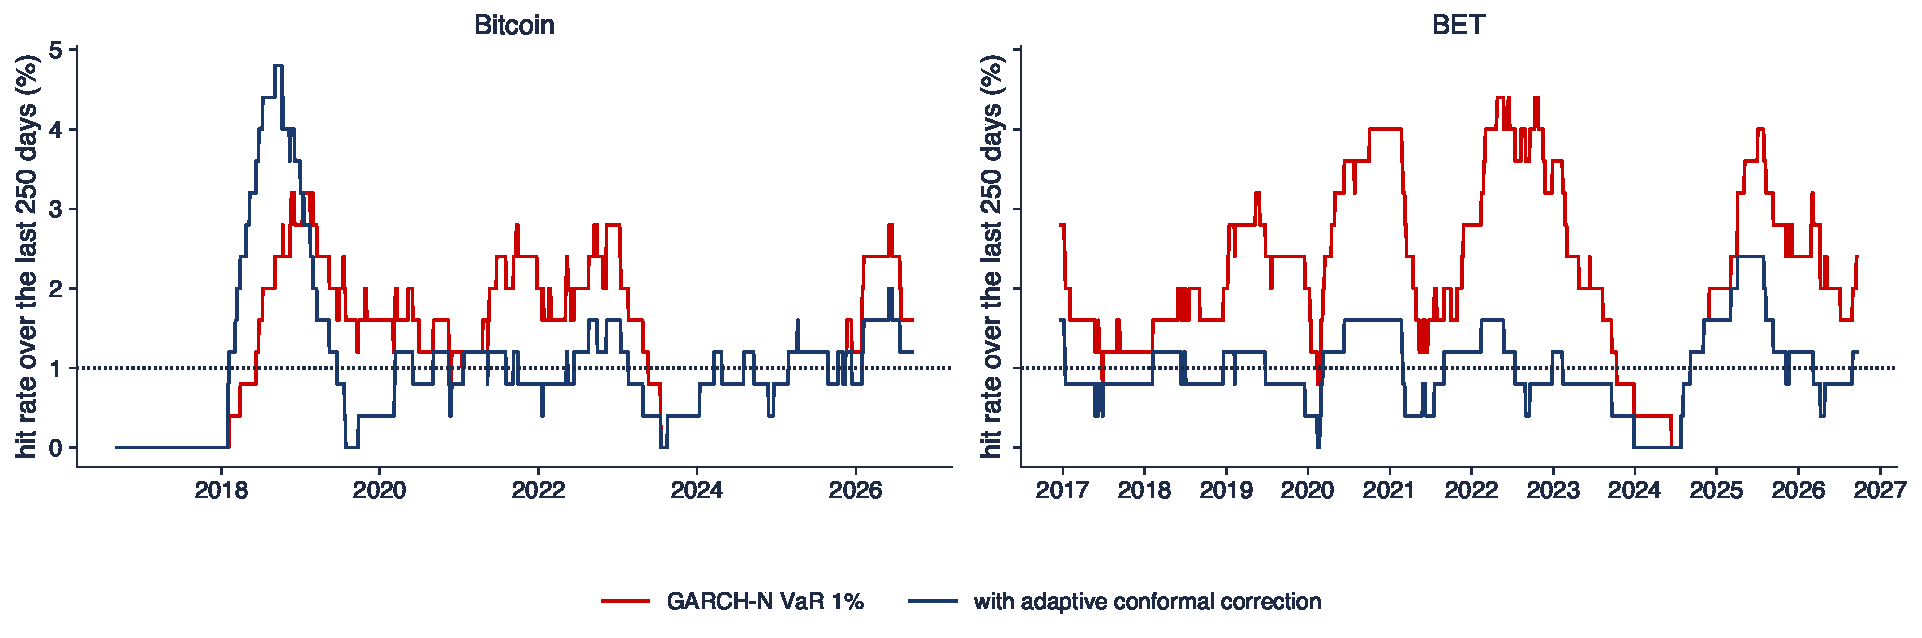
\includegraphics[width=0.97\textwidth,height=0.5\textheight,keepaspectratio]{ats_ch9_conformal.pdf}
\end{center}
\vspace{-0.25cm}
\begin{itemize}
    \item GARCH-N VaR 1\% (rolling 1000-day window, re-estimated every 250 days) from 2016, and its ACI correction with $\gamma$ = 0.005; rolling 250-day hit rates
\end{itemize}
\quantlet{ATS\_ch9\_conformal}{\qlurl{ATS_ch9_conformal}}
\end{frame}

\begin{frame}{Interpreting the conformal correction}
\itemsize{\small}
\begin{itemize}
    \item BET: GARCH-N hits 2.36\% of 2\,675 days (Kupiec $p$ $<$0.001); with ACI 1.08\% ($p$ = 0.666), conditional coverage $p$ = 0.662
    \item Bitcoin: 1.28\% to 1.02\%; the rolling hit rate is not smoothed: its maximum rises from 3.2\% to 4.8\% after over-correction
    \item ACI fixes the frequency, not the dynamics: the adapted level can go below zero (VaR then infinite) after a run of quiet days
    \item A useful wrapper for a regulator's count; a calibrated model is still needed for DQ and for ES
\end{itemize}
\end{frame}

\begin{frame}{Recap: Extremes and conformal calibration}
\itemsize{\small}
\begin{itemize}
    \item Extremes cluster; filtering removes most clustering for liquid markets, not for managed rates
    \item ACI guarantees the long-run hit frequency for any data, nothing more
    \item Both are corrections of a model, not replacements for one
\end{itemize}
\end{frame}


%=============================================================================
\section{AI for scientific discovery}
%=============================================================================

\begin{frame}{An open question}
\itemsize{\small}
\begin{itemize}
    \item Do semiparametric (VaR, ES) models beat location--scale models out of sample once estimation is repeated, and is the advantage concentrated in crises?
    \begin{itemize}
        \item formal: $H_0$: equal expected FZ0 loss of GAS-1F and GARCH-EDF with rolling re-estimation, on pre-registered assets, periods and levels
        \item falsified by a significant GW statistic in the pre-registered crisis windows, robust across $\alpha$ = 1\%, 2.5\%, 5\%
    \end{itemize}
    \item Why it matters: Basel requires ES models; the PZC evidence comes from fixed parameters and four indices
    \begin{itemize}
        \item literature to start from: \refPZC, \refTayB, \refNZ, \refDB
    \end{itemize}
\end{itemize}
\end{frame}

\begin{frame}{The discovery loop with an AI assistant}
\itemsize{\footnotesize}
\begin{itemize}
    \item An AI assistant (an LLM such as Claude, ChatGPT, Gemini or Copilot) speeds up each step; Semantic Scholar and Elicit help with the literature
    \begin{itemize}
        \item \textbf{literature}: \aiprompt{List peer-reviewed papers since 2017 that compare dynamic ES models out of sample with FZ losses; give DOIs.} Then check every DOI on Crossref
        \item \textbf{hypothesis}: \aiprompt{Under which data-generating processes should a one-factor GAS model beat GARCH with empirical innovations for ES 2.5\%?}
        \item \textbf{code and replication}: ask for the GAS-1F recursion, then reproduce a published number first (PZC, Table 8: 0.853)
        \item \textbf{critique}: \aiprompt{Act as a hostile referee: list the ways an FZ0 ranking could be an artefact of the sample, the level or the starting values.}
    \end{itemize}
    \item Report: what was asked, what was kept, what was rejected (AI\_USE.md, AI\_ERRORS.md)
\end{itemize}
\end{frame}

\begin{frame}{What the human checks}
\itemsize{\small}
\begin{itemize}
    \item Every reference exists and says what is claimed (DOI resolves, title matches, the result is in the paper)
    \item The loss is consistent for the target: no ``average ES error'', no MSE of VaR forecasts
    \item The convention is right: VaR 1\% is minus the 1\% quantile of returns, never ``VaR 99\%''; signs of $v$ and $e$ are consistent
    \item Forecasts use only information available at $t - 1$; the estimation window and re-estimation scheme are stated
    \item Rankings are reported with DM or MCS uncertainty and checked on a Murphy diagram
\end{itemize}
\end{frame}

\begin{frame}{Mini-case: is there a best ES model?}
\itemsize{\footnotesize}
\begin{center}
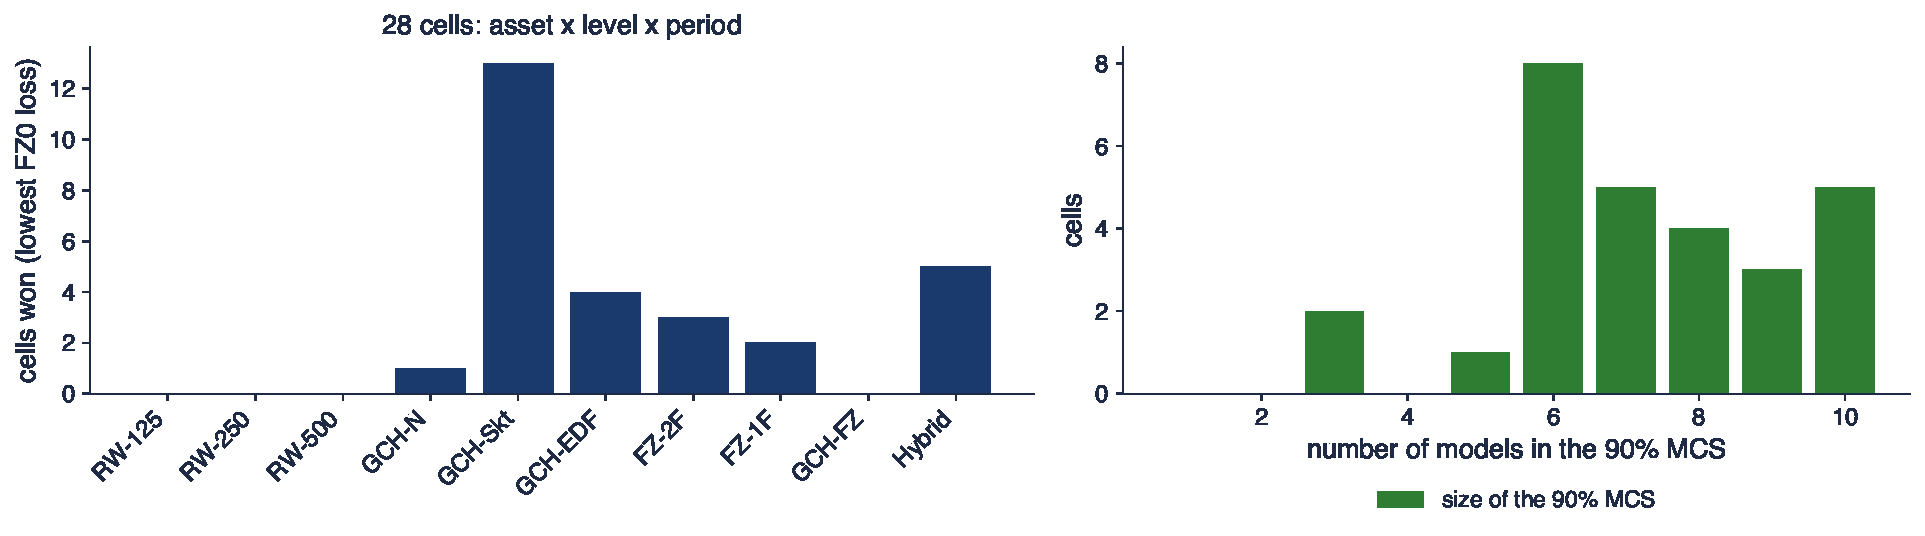
\includegraphics[width=0.97\textwidth,height=0.44\textheight,keepaspectratio]{ats_ch9_ai_case.pdf}
\end{center}
\vspace{-0.25cm}
\begin{itemize}
    \item 28 cells: five assets $\times$ two levels (2.5\%, 5\%) $\times$ up to three periods (whole, before 2020, from 2020); left: the model with the lowest FZ0 loss; right: size of the 90\% MCS
    \item 6 different winners; GARCH-Skt wins 13 cells, GAS-1F 2; MCS sizes from 3 to 10, median 7; GAS-1F is in the MCS in 22 cells: an AI summary that names ``the best ES model'' is wrong
\end{itemize}
\quantlet{ATS\_ch9\_comparison}{\qlurl{ATS_ch9_comparison}}
\end{frame}

\begin{frame}{Project idea}
\itemsize{\small}
\begin{itemize}
    \item \textbf{ES models for Central and Eastern European markets under rolling re-estimation}: replicate first, then extend
    \begin{itemize}
        \item replicate: PZC Table 8 and Table S5 for the S\&P 500 (GAS-1F 0.853 and 1.032) and the EM design with VaR 1\%
        \item extend: BET, WIG20, BUX, PX and EUR/RON; rolling re-estimation; joint (VaR, ES) regressions with VIX and the BNR rate; ACI as a wrapper
        \item pre-register: samples, levels, models, windows, the stress periods and the MCS design
    \end{itemize}
    \item Deliverables follow the course rules: repository, report, AI\_USE.md, AI\_ERRORS.md, oral defence
\end{itemize}
\end{frame}


%=============================================================================
\section{Wrap-up}
%=============================================================================

\begin{frame}{Key takeaways}
\itemsize{\small}
\begin{itemize}
    \item A risk forecast is a point forecast of a functional; judge it with a loss consistent for that functional
    \item VaR is elicitable, ES only with VaR; FZ0 is the scale-free choice for time series
    \item CAViaR and GAS-FZ models estimate the tail directly; their published rankings replicate, their published tests do not
    \item Backtests are moment tests with estimation risk; comparisons need DM, MCS and Murphy diagrams
    \item Horizon, model and estimation risk are larger than most reported confidence suggests
\end{itemize}
\end{frame}

\begin{frame}{Self-assessment}
\itemsize{\small}
\begin{columns}[T]
\begin{column}{0.56\textwidth}
\begin{block}{Questions}
\begin{itemize}
    \item Why does a non-convex level set rule out a strictly consistent loss for ES?
    \item Which choice of $(G_1, G_2)$ gives FZ0, and what does zero homogeneity buy?
    \item Why is the DQ test with a VaR regressor more powerful than Christoffersen's test?
    \item Why does a fixed estimation window inflate the size of the Kupiec test?
    \item When does $\sqrt{10}$ scaling overstate the 10-day VaR?
\end{itemize}
\end{block}
\end{column}
\begin{column}{0.40\textwidth}
\begin{block}{Next: \atschlink{https://danpele.github.io/Advanced-Time-Series/EN/Courses/chapter10_long_memory_rough_volatility.pdf}{Chapter 10}}
\begin{itemize}
    \item Long memory and rough volatility
    \item ARFIMA, fractional cointegration, rough volatility
\end{itemize}
\end{block}
\end{column}
\end{columns}
\end{frame}


%=============================================================================
\section{Appendix}
%=============================================================================

\begin{frame}{Appendix: consistency of GPL quantile scores}
\hypertarget{atsapp1}{}\atsappback{atssrc1}{Back}
\itemsize{\small}
\begin{itemize}
    \item The expected GPL score of a report $x$ under $Y \sim F$
    \[ \E_F S(x, Y) = \int_{-\infty}^x(1 - \alpha)(G(x) - G(y))\,dF(y) + \int_x^\infty \alpha(G(y) - G(x))\,dF(y) \]
    \item Differentiate (Leibniz; the boundary terms vanish)
    \[ \frac{d}{dx}\E_F S(x, Y) = G'(x)\big[(1 - \alpha)F(x) - \alpha(1 - F(x))\big] = G'(x)(F(x) - \alpha) \]
    \item $G' \ge 0$: the derivative is $\le 0$ for $x < q_\alpha$ and $\ge 0$ for $x > q_\alpha$, so $q_\alpha$ minimises; strictly if $G$ is strictly increasing and $F$ has a unique $\alpha$-quantile
    \item The same computation with $G(x) = x$ is the first-order condition of quantile regression
\end{itemize}
\end{frame}

\begin{frame}{Appendix: FZ0, consistency and homogeneity}
\hypertarget{atsapp2}{}\atsappback{atssrc2}{Back}
\itemsize{\small}
\begin{itemize}
    \item Fix $e$; in $v$, FZ0 is $-\frac{1}{\alpha e}\big[\mathbf 1\{y \le v\}(v - y) - \alpha v\big]$ plus terms free of $v$: since $-1/(\alpha e) > 0$, a positive multiple of the pinball loss, minimised at $q_\alpha$
    \item At $v = q_\alpha$: $\E\,L = \dfrac{c}{e} + \ln(-e) - 1$ with $c = v - \frac1\alpha\E[\mathbf 1\{Y \le v\}(v - Y)] = \E[Y \mid Y \le q_\alpha] = -\mathrm{ES}_\alpha$; the derivative $-c/e^2 + 1/e$ vanishes at $e = c$
    \item Homogeneity: replacing $(y, v, e)$ by $(sy, sv, se)$, $s > 0$, changes FZ0 only by $\ln s$, the same for every forecast: loss differences are scale-free
    \item Joint minimisation over $(v, e)$ with $e \le v < 0$ therefore returns $(q_\alpha, -\mathrm{ES}_\alpha)$
\end{itemize}
\end{frame}


%=============================================================================
\section{References}
%=============================================================================

\begin{frame}{References (1/4)}
\itemsize{\tiny}
\begin{itemize}
    \item Acerbi, C., \& Székely, B. (2014). Backtesting expected shortfall. \textit{Risk}, December 2014 (MSCI working paper). \href{https://www.msci.com/documents/10199/22aa9922-f874-4060-b77a-0f0e267a489b}{msci.com}
    \item Acerbi, C., \& Tasche, D. (2002). On the coherence of expected shortfall. \textit{Journal of Banking \& Finance}, 26(7), 1487--1503. \href{https://doi.org/10.1016/S0378-4266(02)00283-2}{doi:10.1016/S0378-4266(02)00283-2}
    \item Artzner, P., Delbaen, F., Eber, J.-M., \& Heath, D. (1999). Coherent measures of risk. \textit{Mathematical Finance}, 9(3), 203--228. \href{https://doi.org/10.1111/1467-9965.00068}{doi:10.1111/1467-9965.00068}
    \item Basel Committee on Banking Supervision (2019). \textit{MAR33: Internal models approach, capital requirements calculation}. Basel Framework, Bank for International Settlements. \href{https://www.bis.org/basel_framework/chapter/MAR/33.htm}{bis.org}
    \item Basel Committee on Banking Supervision (1996). \textit{Supervisory framework for the use of ``backtesting in conjunction with the internal models approach to market risk capital requirements}. Bank for International Settlements. \href{https://www.bis.org/publ/bcbs22.htm}{bis.org}
    \item Bayer, S., \& Dimitriadis, T. (2022). Regression-based expected shortfall backtesting. \textit{Journal of Financial Econometrics}, 20(3), 437--471. \href{https://doi.org/10.1093/jjfinec/nbaa013}{doi:10.1093/jjfinec/nbaa013}
    \item Bollerslev, T. (1986). Generalized autoregressive conditional heteroskedasticity. \textit{Journal of Econometrics}, 31(3), 307--327. \href{https://doi.org/10.1016/0304-4076(86)90063-1}{doi:10.1016/0304-4076(86)90063-1}
    \item Boucher, C. M., Daníelsson, J., Kouontchou, P. S., \& Maillet, B. B. (2014). Risk models-at-risk. \textit{Journal of Banking \& Finance}, 44, 72--92. \href{https://doi.org/10.1016/j.jbankfin.2014.03.019}{doi:10.1016/j.jbankfin.2014.03.019}
    \item Christoffersen, P. F. (1998). Evaluating interval forecasts. \textit{International Economic Review}, 39(4), 841--862. \href{https://doi.org/10.2307/2527341}{doi:10.2307/2527341}
    \item Christoffersen, P., \& Gonçalves, S. (2005). Estimation risk in financial risk management. \textit{The Journal of Risk}, 7(3), 1--28. \href{https://doi.org/10.21314/JOR.2005.112}{doi:10.21314/JOR.2005.112}
    \item Christoffersen, P., \& Pelletier, D. (2004). Backtesting value-at-risk: A duration-based approach. \textit{Journal of Financial Econometrics}, 2(1), 84--108. \href{https://doi.org/10.1093/jjfinec/nbh004}{doi:10.1093/jjfinec/nbh004}
    \item Creal, D., Koopman, S. J., \& Lucas, A. (2013). Generalized autoregressive score models with applications. \textit{Journal of Applied Econometrics}, 28(5), 777--795. \href{https://doi.org/10.1002/jae.1279}{doi:10.1002/jae.1279}
    \item Daníelsson, J., \& Zigrand, J.-P. (2006). On time-scaling of risk and the square-root-of-time rule. \textit{Journal of Banking \& Finance}, 30(10), 2701--2713. \href{https://doi.org/10.1016/j.jbankfin.2005.10.002}{doi:10.1016/j.jbankfin.2005.10.002}
\end{itemize}
\end{frame}

\begin{frame}{References (2/4)}
\itemsize{\tiny}
\begin{itemize}
    \item Danielsson, J., James, K. R., Valenzuela, M., \& Zer, I. (2016). Model risk of risk models. \textit{Journal of Financial Stability}, 23, 79--91. \href{https://doi.org/10.1016/j.jfs.2016.02.002}{doi:10.1016/j.jfs.2016.02.002}
    \item Diebold, F. X., \& Mariano, R. S. (1995). Comparing predictive accuracy. \textit{Journal of Business \& Economic Statistics}, 13(3), 253--263. \href{https://doi.org/10.1080/07350015.1995.10524599}{doi:10.1080/07350015.1995.10524599}
    \item Dimitriadis, T., \& Bayer, S. (2019). A joint quantile and expected shortfall regression framework. \textit{Electronic Journal of Statistics}, 13(1), 1823--1871. \href{https://doi.org/10.1214/19-EJS1560}{doi:10.1214/19-EJS1560}
    \item Du, Z., \& Escanciano, J. C. (2017). Backtesting expected shortfall: Accounting for tail risk. \textit{Management Science}, 63(4), 940--958. \href{https://doi.org/10.1287/mnsc.2015.2342}{doi:10.1287/mnsc.2015.2342}
    \item Ehm, W., Gneiting, T., Jordan, A., \& Krüger, F. (2016). Of quantiles and expectiles: Consistent scoring functions, Choquet representations and forecast rankings. \textit{Journal of the Royal Statistical Society: Series B}, 78(3), 505--562. \href{https://doi.org/10.1111/rssb.12154}{doi:10.1111/rssb.12154}
    \item Embrechts, P., Klüppelberg, C., \& Mikosch, T. (1997). \textit{Modelling Extremal Events for Insurance and Finance}. Springer. \href{https://doi.org/10.1007/978-3-642-33483-2}{doi:10.1007/978-3-642-33483-2}
    \item Engle, R. F., \& Manganelli, S. (2004). CAViaR: Conditional autoregressive value at risk by regression quantiles. \textit{Journal of Business \& Economic Statistics}, 22(4), 367--381. \href{https://doi.org/10.1198/073500104000000370}{doi:10.1198/073500104000000370}
    \item Escanciano, J. C., \& Olmo, J. (2010). Backtesting parametric value-at-risk with estimation risk. \textit{Journal of Business \& Economic Statistics}, 28(1), 36--51. \href{https://doi.org/10.1198/jbes.2009.07063}{doi:10.1198/jbes.2009.07063}
    \item Ferro, C. A. T., \& Segers, J. (2003). Inference for clusters of extreme values. \textit{Journal of the Royal Statistical Society: Series B}, 65(2), 545--556. \href{https://doi.org/10.1111/1467-9868.00401}{doi:10.1111/1467-9868.00401}
    \item Fissler, T., Ziegel, J. F., \& Gneiting, T. (2016). Expected shortfall is jointly elicitable with value at risk: Implications for backtesting. \textit{Risk}, January 2016, 58--61; arXiv:1507.00244. \href{https://arxiv.org/abs/1507.00244}{arxiv.org}
    \item Fissler, T., \& Ziegel, J. F. (2016). Higher order elicitability and Osband's principle. \textit{The Annals of Statistics}, 44(4), 1680--1707. \href{https://doi.org/10.1214/16-AOS1439}{doi:10.1214/16-AOS1439}
    \item Gaglianone, W. P., Lima, L. R., Linton, O., \& Smith, D. R. (2011). Evaluating value-at-risk models via quantile regression. \textit{Journal of Business \& Economic Statistics}, 29(1), 150--160. \href{https://doi.org/10.1198/jbes.2010.07318}{doi:10.1198/jbes.2010.07318}
    \item Gao, F., \& Song, F. (2008). Estimation risk in GARCH VaR and ES estimates. \textit{Econometric Theory}, 24(5), 1404--1424. \href{https://doi.org/10.1017/S0266466608080559}{doi:10.1017/S0266466608080559}
\end{itemize}
\end{frame}

\begin{frame}{References (3/4)}
\itemsize{\tiny}
\begin{itemize}
    \item Giacomini, R., \& White, H. (2006). Tests of conditional predictive ability. \textit{Econometrica}, 74(6), 1545--1578. \href{https://doi.org/10.1111/j.1468-0262.2006.00718.x}{doi:10.1111/j.1468-0262.2006.00718.x}
    \item Gibbs, I., \& Candès, E. (2021). Adaptive conformal inference under distribution shift. \textit{Advances in Neural Information Processing Systems}, 34; arXiv:2106.00170. \href{https://arxiv.org/abs/2106.00170}{arxiv.org}
    \item Glosten, L. R., Jagannathan, R., \& Runkle, D. E. (1993). On the relation between the expected value and the volatility of the nominal excess return on stocks. \textit{The Journal of Finance}, 48(5), 1779--1801. \href{https://doi.org/10.1111/j.1540-6261.1993.tb05128.x}{doi:10.1111/j.1540-6261.1993.tb05128.x}
    \item Gneiting, T. (2011). Making and evaluating point forecasts. \textit{Journal of the American Statistical Association}, 106(494), 746--762. \href{https://doi.org/10.1198/jasa.2011.r10138}{doi:10.1198/jasa.2011.r10138}
    \item Gneiting, T., \& Raftery, A. E. (2007). Strictly proper scoring rules, prediction, and estimation. \textit{Journal of the American Statistical Association}, 102(477), 359--378. \href{https://doi.org/10.1198/016214506000001437}{doi:10.1198/016214506000001437}
    \item Hansen, B. E. (1994). Autoregressive conditional density estimation. \textit{International Economic Review}, 35(3), 705--730. \href{https://doi.org/10.2307/2527081}{doi:10.2307/2527081}
    \item Hansen, P. R., Lunde, A., \& Nason, J. M. (2011). The model confidence set. \textit{Econometrica}, 79(2), 453--497. \href{https://doi.org/10.3982/ECTA5771}{doi:10.3982/ECTA5771}
    \item Holzmann, H., \& Eulert, M. (2014). The role of the information set for forecasting -- with applications to risk management. \textit{The Annals of Applied Statistics}, 8(1), 595--621. \href{https://doi.org/10.1214/13-AOAS709}{doi:10.1214/13-AOAS709}
    \item Kellner, R., \& Rösch, D. (2016). Quantifying market risk with value-at-risk or expected shortfall? Consequences for capital requirements and model risk. \textit{Journal of Economic Dynamics and Control}, 68, 45--63. \href{https://doi.org/10.1016/j.jedc.2016.05.002}{doi:10.1016/j.jedc.2016.05.002}
    \item Koenker, R., \& Bassett, G. (1978). Regression quantiles. \textit{Econometrica}, 46(1), 33--50. \href{https://doi.org/10.2307/1913643}{doi:10.2307/1913643}
    \item Koenker, R. (2005). \textit{Quantile Regression}. Cambridge University Press. \href{https://doi.org/10.1017/CBO9780511754098}{doi:10.1017/CBO9780511754098}
    \item Koenker, R., \& Xiao, Z. (2006). Quantile autoregression. \textit{Journal of the American Statistical Association}, 101(475), 980--990. \href{https://doi.org/10.1198/016214506000000672}{doi:10.1198/016214506000000672}
    \item Kratz, M., Lok, Y. H., \& McNeil, A. J. (2018). Multinomial VaR backtests: A simple implicit approach to backtesting expected shortfall. \textit{Journal of Banking \& Finance}, 88, 393--407. \href{https://doi.org/10.1016/j.jbankfin.2018.01.002}{doi:10.1016/j.jbankfin.2018.01.002}
\end{itemize}
\end{frame}

\begin{frame}{References (4/4)}
\itemsize{\tiny}
\begin{itemize}
    \item Kupiec, P. H. (1995). Techniques for verifying the accuracy of risk measurement models. \textit{The Journal of Derivatives}, 3(2), 73--84. \href{https://doi.org/10.3905/jod.1995.407942}{doi:10.3905/jod.1995.407942}
    \item McNeil, A. J., \& Frey, R. (2000). Estimation of tail-related risk measures for heteroscedastic financial time series: An extreme value approach. \textit{Journal of Empirical Finance}, 7(3--4), 271--300. \href{https://doi.org/10.1016/S0927-5398(00)00012-8}{doi:10.1016/S0927-5398(00)00012-8}
    \item Nolde, N., \& Ziegel, J. F. (2017). Elicitability and backtesting: Perspectives for banking regulation. \textit{The Annals of Applied Statistics}, 11(4), 1833--1874. \href{https://doi.org/10.1214/17-AOAS1041}{doi:10.1214/17-AOAS1041}
    \item Patton, A. J., Ziegel, J. F., \& Chen, R. (2019). Dynamic semiparametric models for expected shortfall (and value-at-risk). \textit{Journal of Econometrics}, 211(2), 388--413. \href{https://doi.org/10.1016/j.jeconom.2018.10.008}{doi:10.1016/j.jeconom.2018.10.008}
    \item Pele, D. T., Bolovăneanu, V., Ginavar, A., Lessmann, S., \& Härdle, W. K. Conformal recalibration of extreme tail quantiles under temporal dependence. Working paper and replication package (further reading). \href{https://github.com/danpele/Conformal_Oracle}{github.com}
    \item Petropoulos, F., Apiletti, D., Assimakopoulos, V., Babai, M. Z., et al.\ (2022). Forecasting: Theory and practice. \textit{International Journal of Forecasting}, 38(3), 705--871. \href{https://doi.org/10.1016/j.ijforecast.2021.11.001}{doi:10.1016/j.ijforecast.2021.11.001}
    \item Taylor, J. W. (2008). Estimating value at risk and expected shortfall using expectiles. \textit{Journal of Financial Econometrics}, 6(2), 231--252. \href{https://doi.org/10.1093/jjfinec/nbn001}{doi:10.1093/jjfinec/nbn001}
    \item Taylor, J. W. (2019). Forecasting value at risk and expected shortfall using a semiparametric approach based on the asymmetric Laplace distribution. \textit{Journal of Business \& Economic Statistics}, 37(1), 121--133. \href{https://doi.org/10.1080/07350015.2017.1281815}{doi:10.1080/07350015.2017.1281815}
    \item Weber, S. (2006). Distribution-invariant risk measures, information, and dynamic consistency. \textit{Mathematical Finance}, 16(2), 419--441. \href{https://doi.org/10.1111/j.1467-9965.2006.00277.x}{doi:10.1111/j.1467-9965.2006.00277.x}
    \item Ziegel, J. F. (2016). Coherence and elicitability. \textit{Mathematical Finance}, 26(4), 901--918. \href{https://doi.org/10.1111/mafi.12080}{doi:10.1111/mafi.12080}
\end{itemize}
\end{frame}

\end{document}
